\section{Discussion of the results}
We conducted 2 main types of measurements: the first ones are intended to check whether our simulation is compatible with the theoretical predictions, then we started studying the network behavior. We will now discuss these results using different types of networks.
\subsection{Seeking the phase transition}
To understand if our simulations agree with the theoretical predictions, we compared the phase transition temperatures (measured) with the predicted one from theory. Since the measuring procedure for these quantities is not so computationally heavy, we let the simulation thermalize for longer times, taking more measures, and we also used bigger lattices.

We simulated, with $J=50$, a square lattice of 900 atoms, a triangular lattice of 496 atoms and a hexagonal lattice of 38 atoms. At each temperature we obtained an ensemble of 3000 systems, one every 100 steps. The agreement between the model and the simulation is appreciable from Figure \ref{Fig:Behaviour1}, \ref{Fig:Behaviour2} and \ref{Fig:Behaviour3}, which show the phase transition in the magnetization, the entropy, in the susceptibility and in the heat capacity.

\begin{figure}[!htb]
    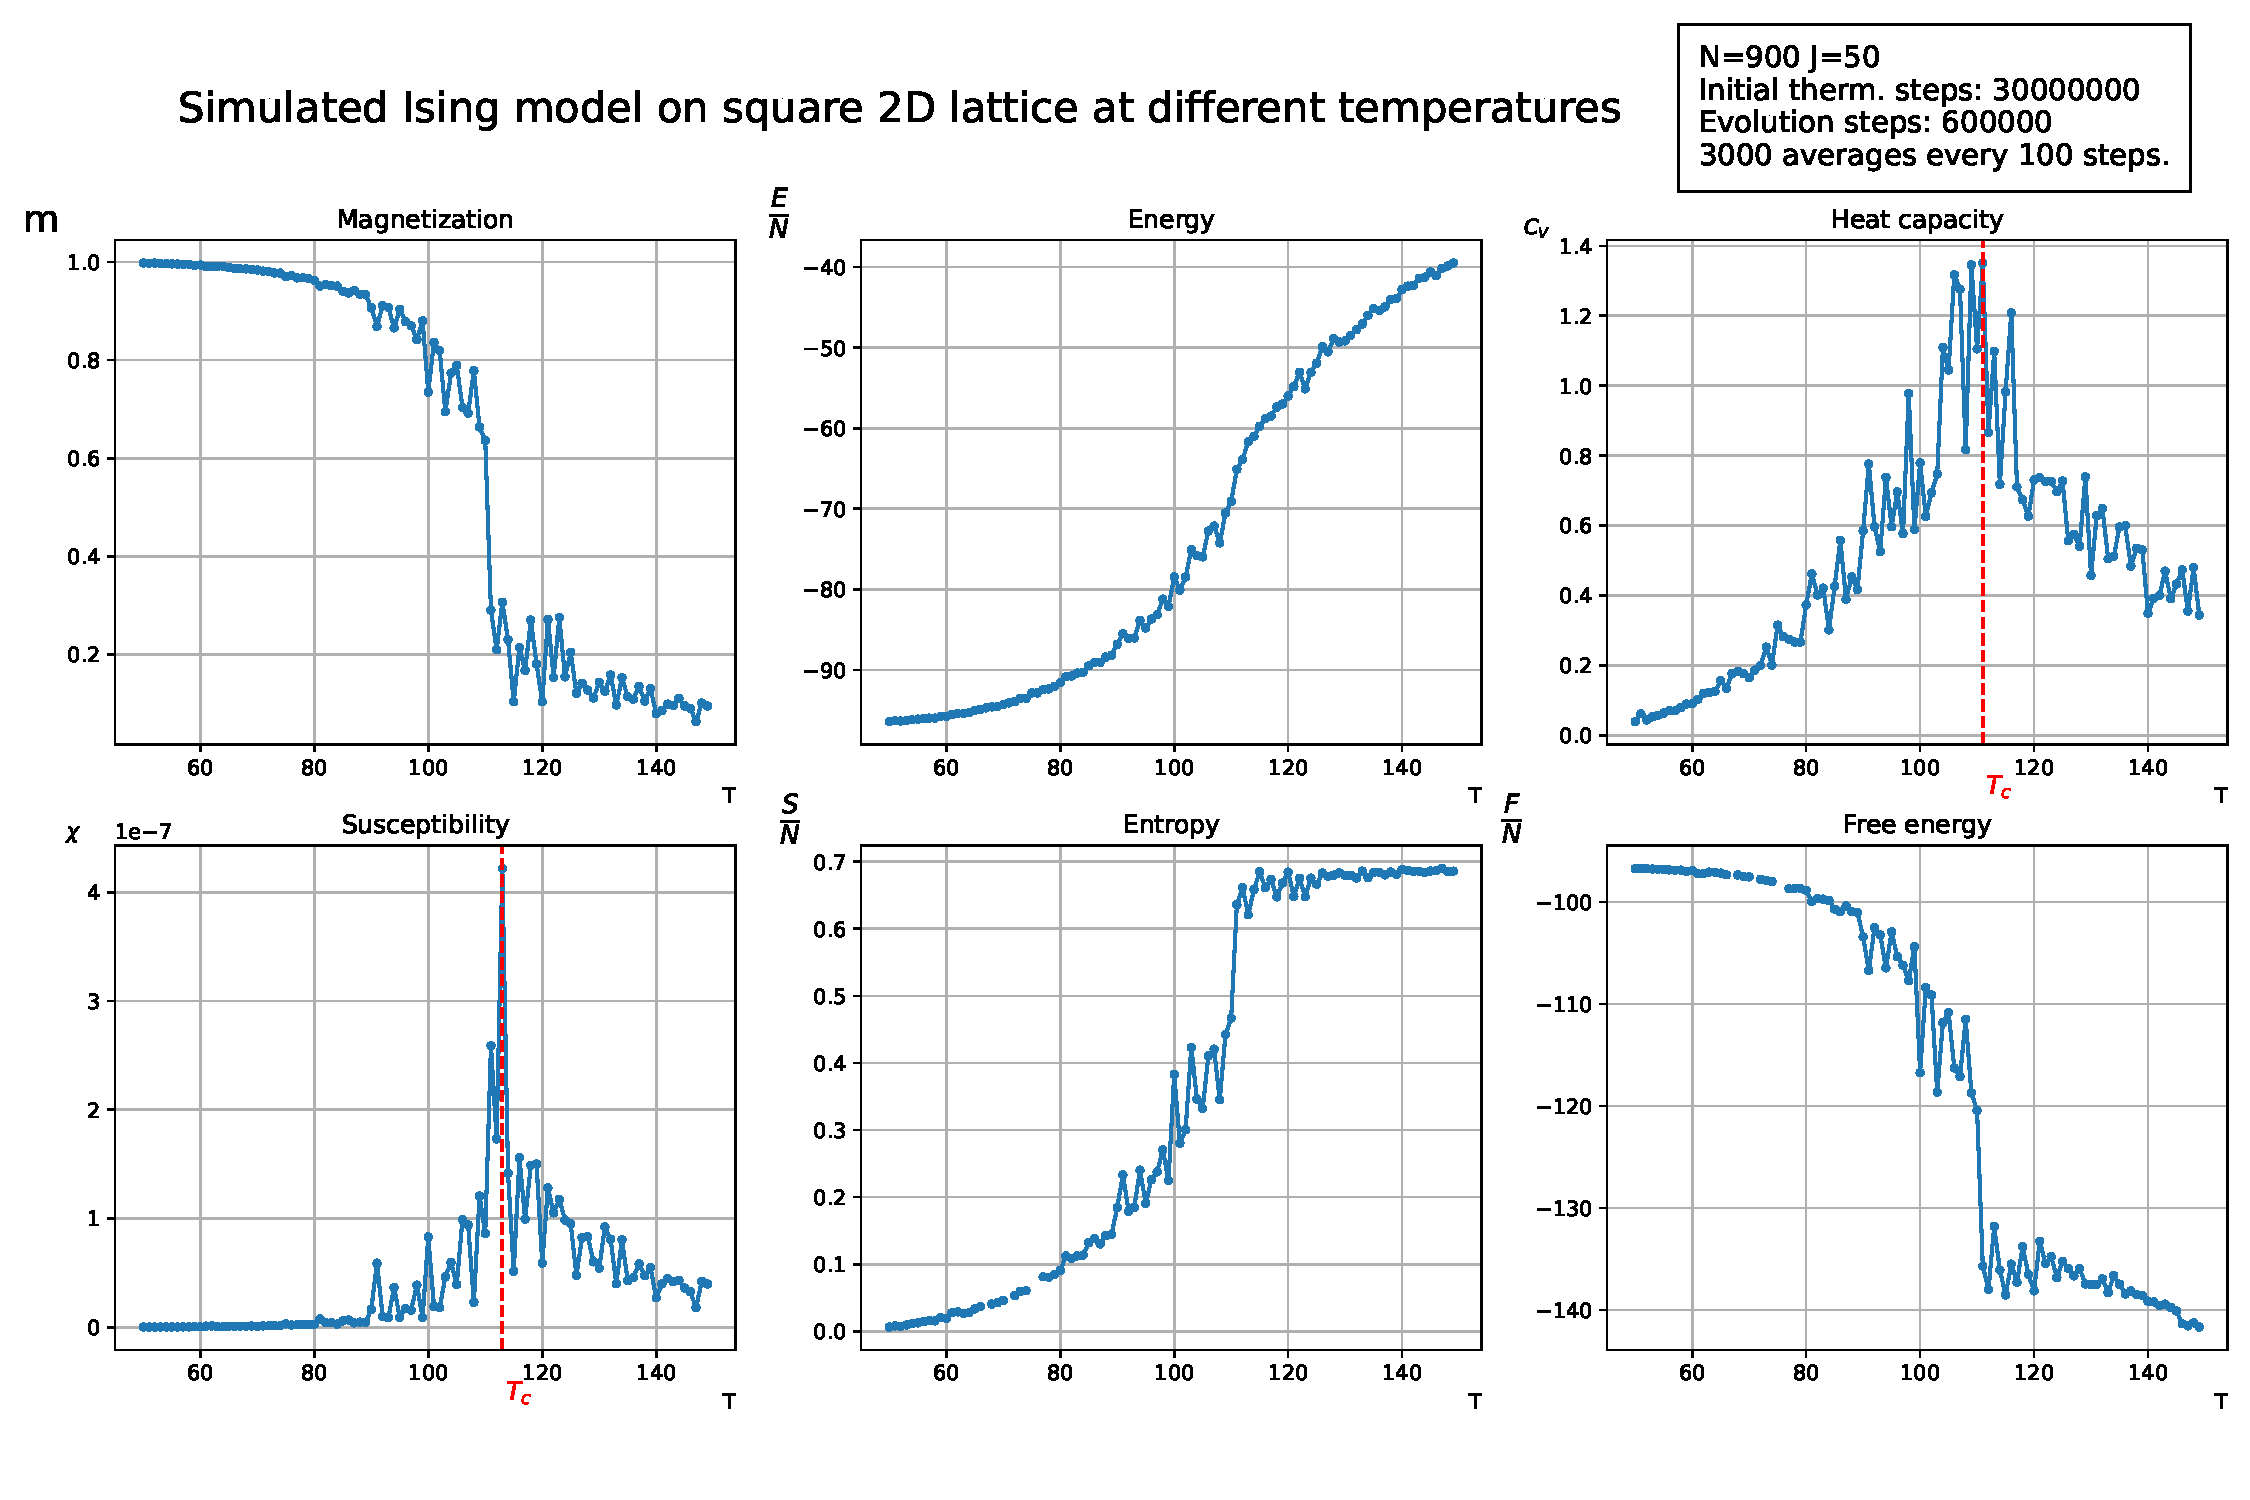
\includegraphics[width=\linewidth]{2d_square_thermal.pdf}
      \caption{Behavior of the square lattice at increasing temperatures. We highlighted with a dashed line the critical temperatures we measured.}\label{Fig:Behaviour1}
\end{figure}

\begin{figure}[!htb] 
    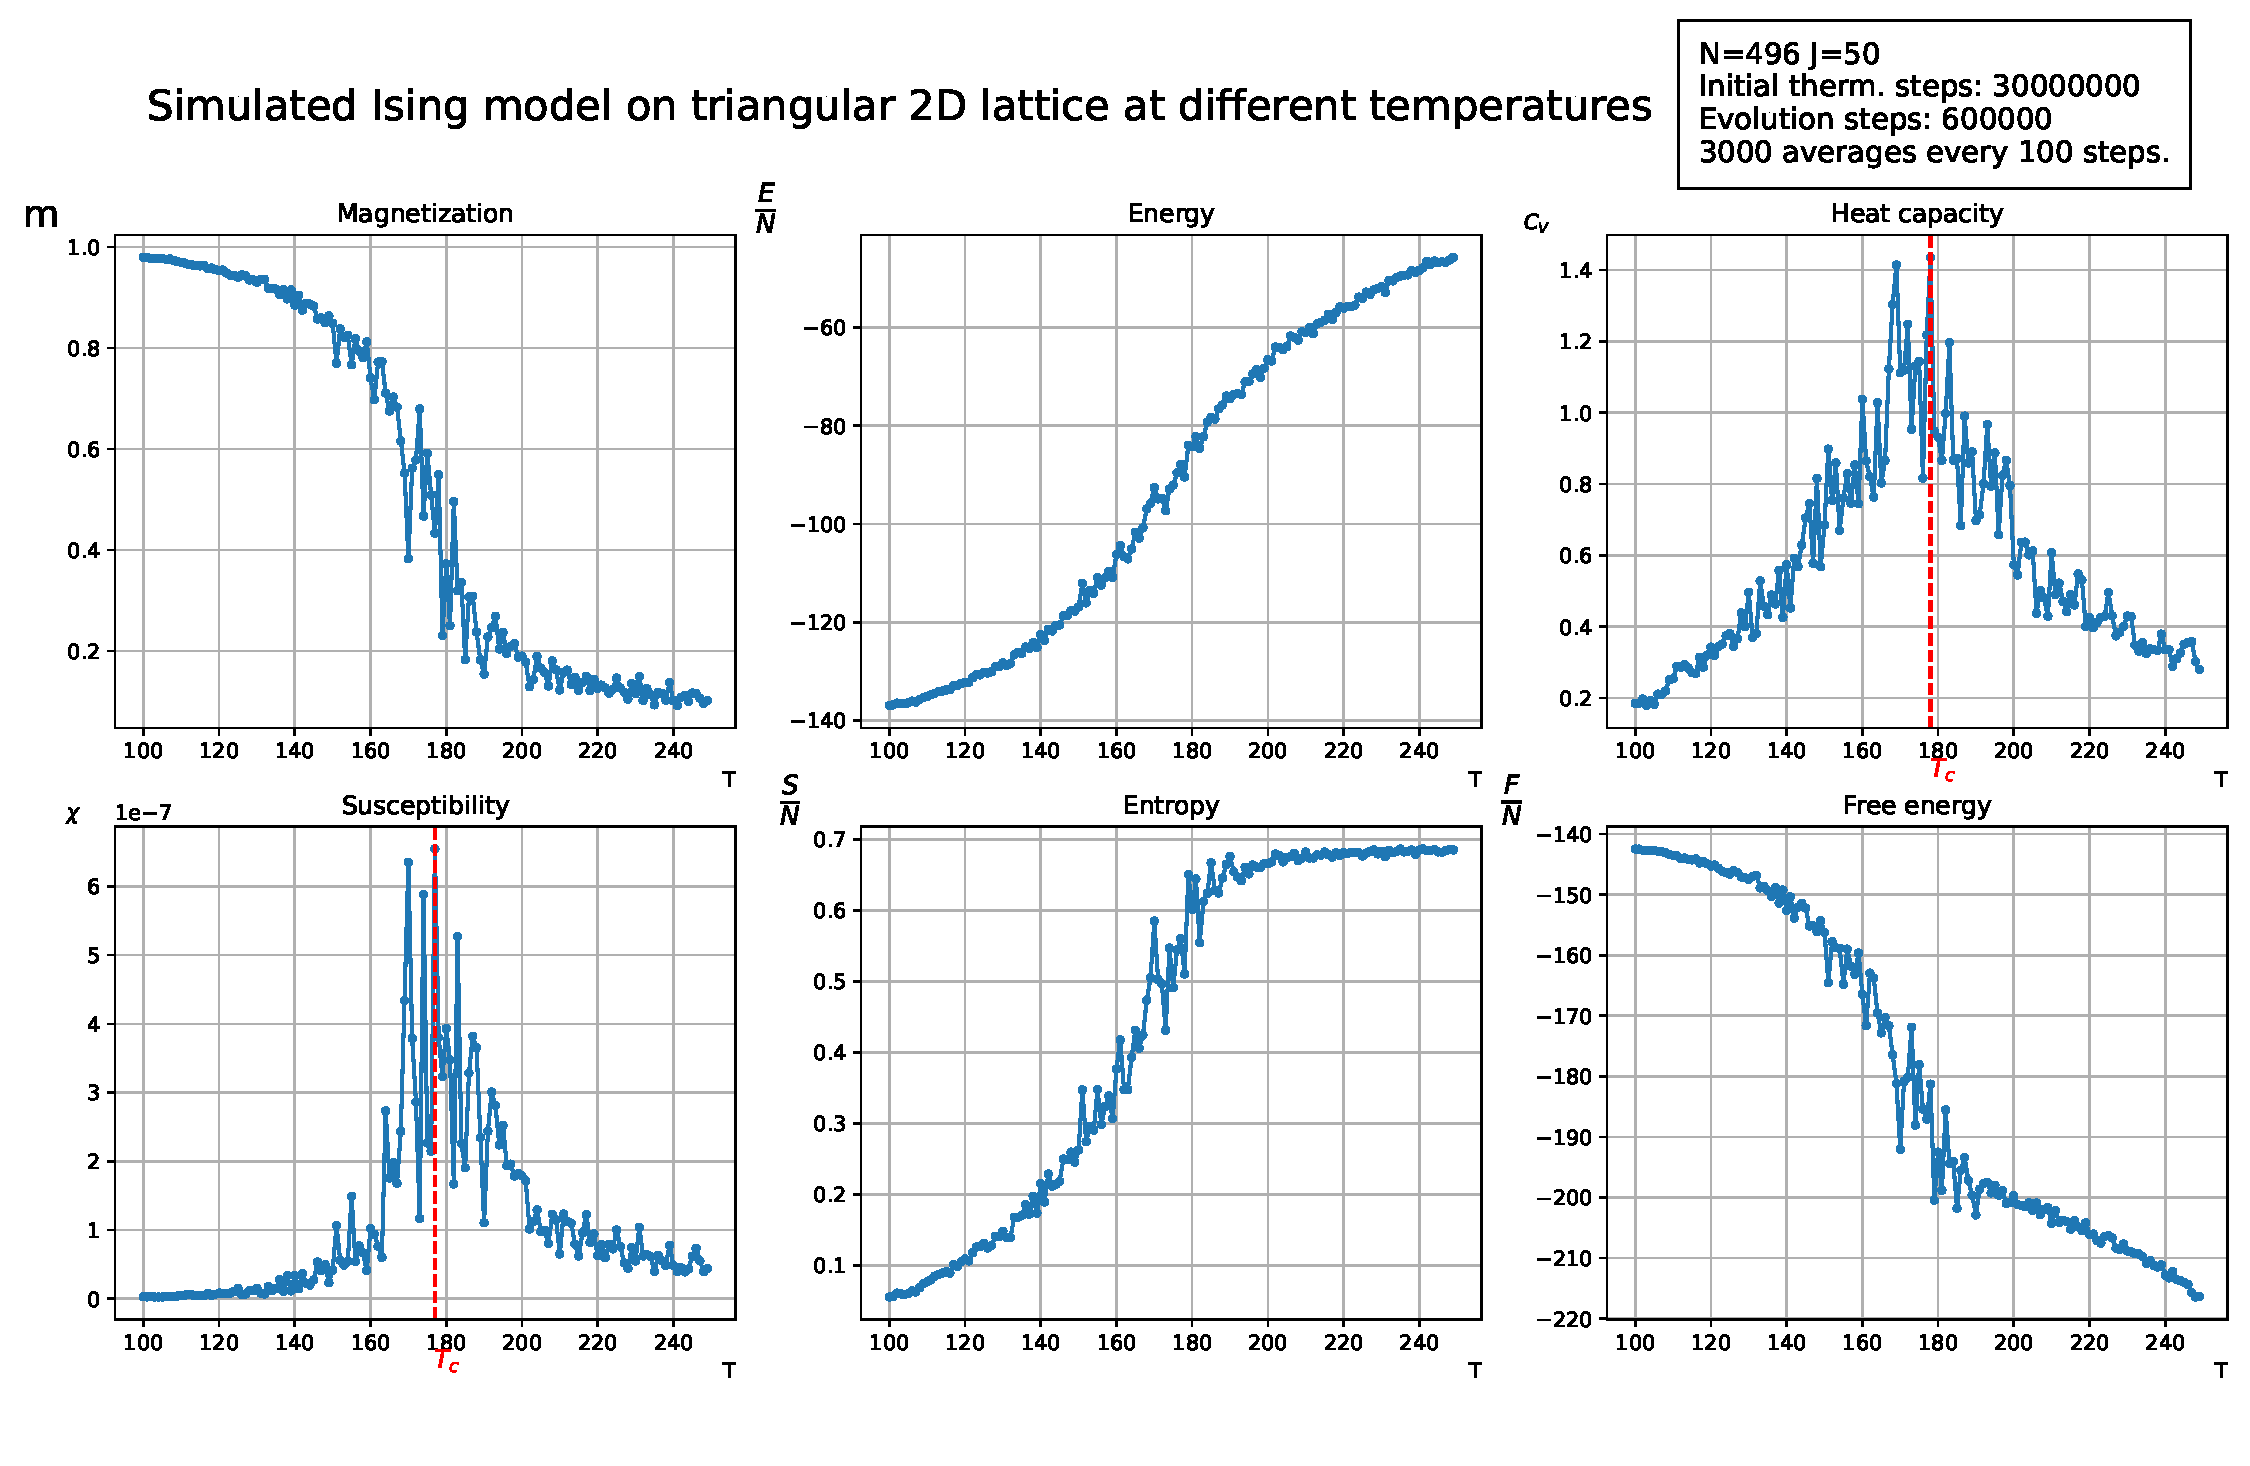
\includegraphics[width=\linewidth]{2d_triangular_thermal.pdf}
      \caption{Behavior of the triangular lattice at increasing temperatures. We highlighted with a dashed line the critical temperatures we measured.}\label{Fig:Behaviour2}
\end{figure}

\begin{figure}[!htb]
    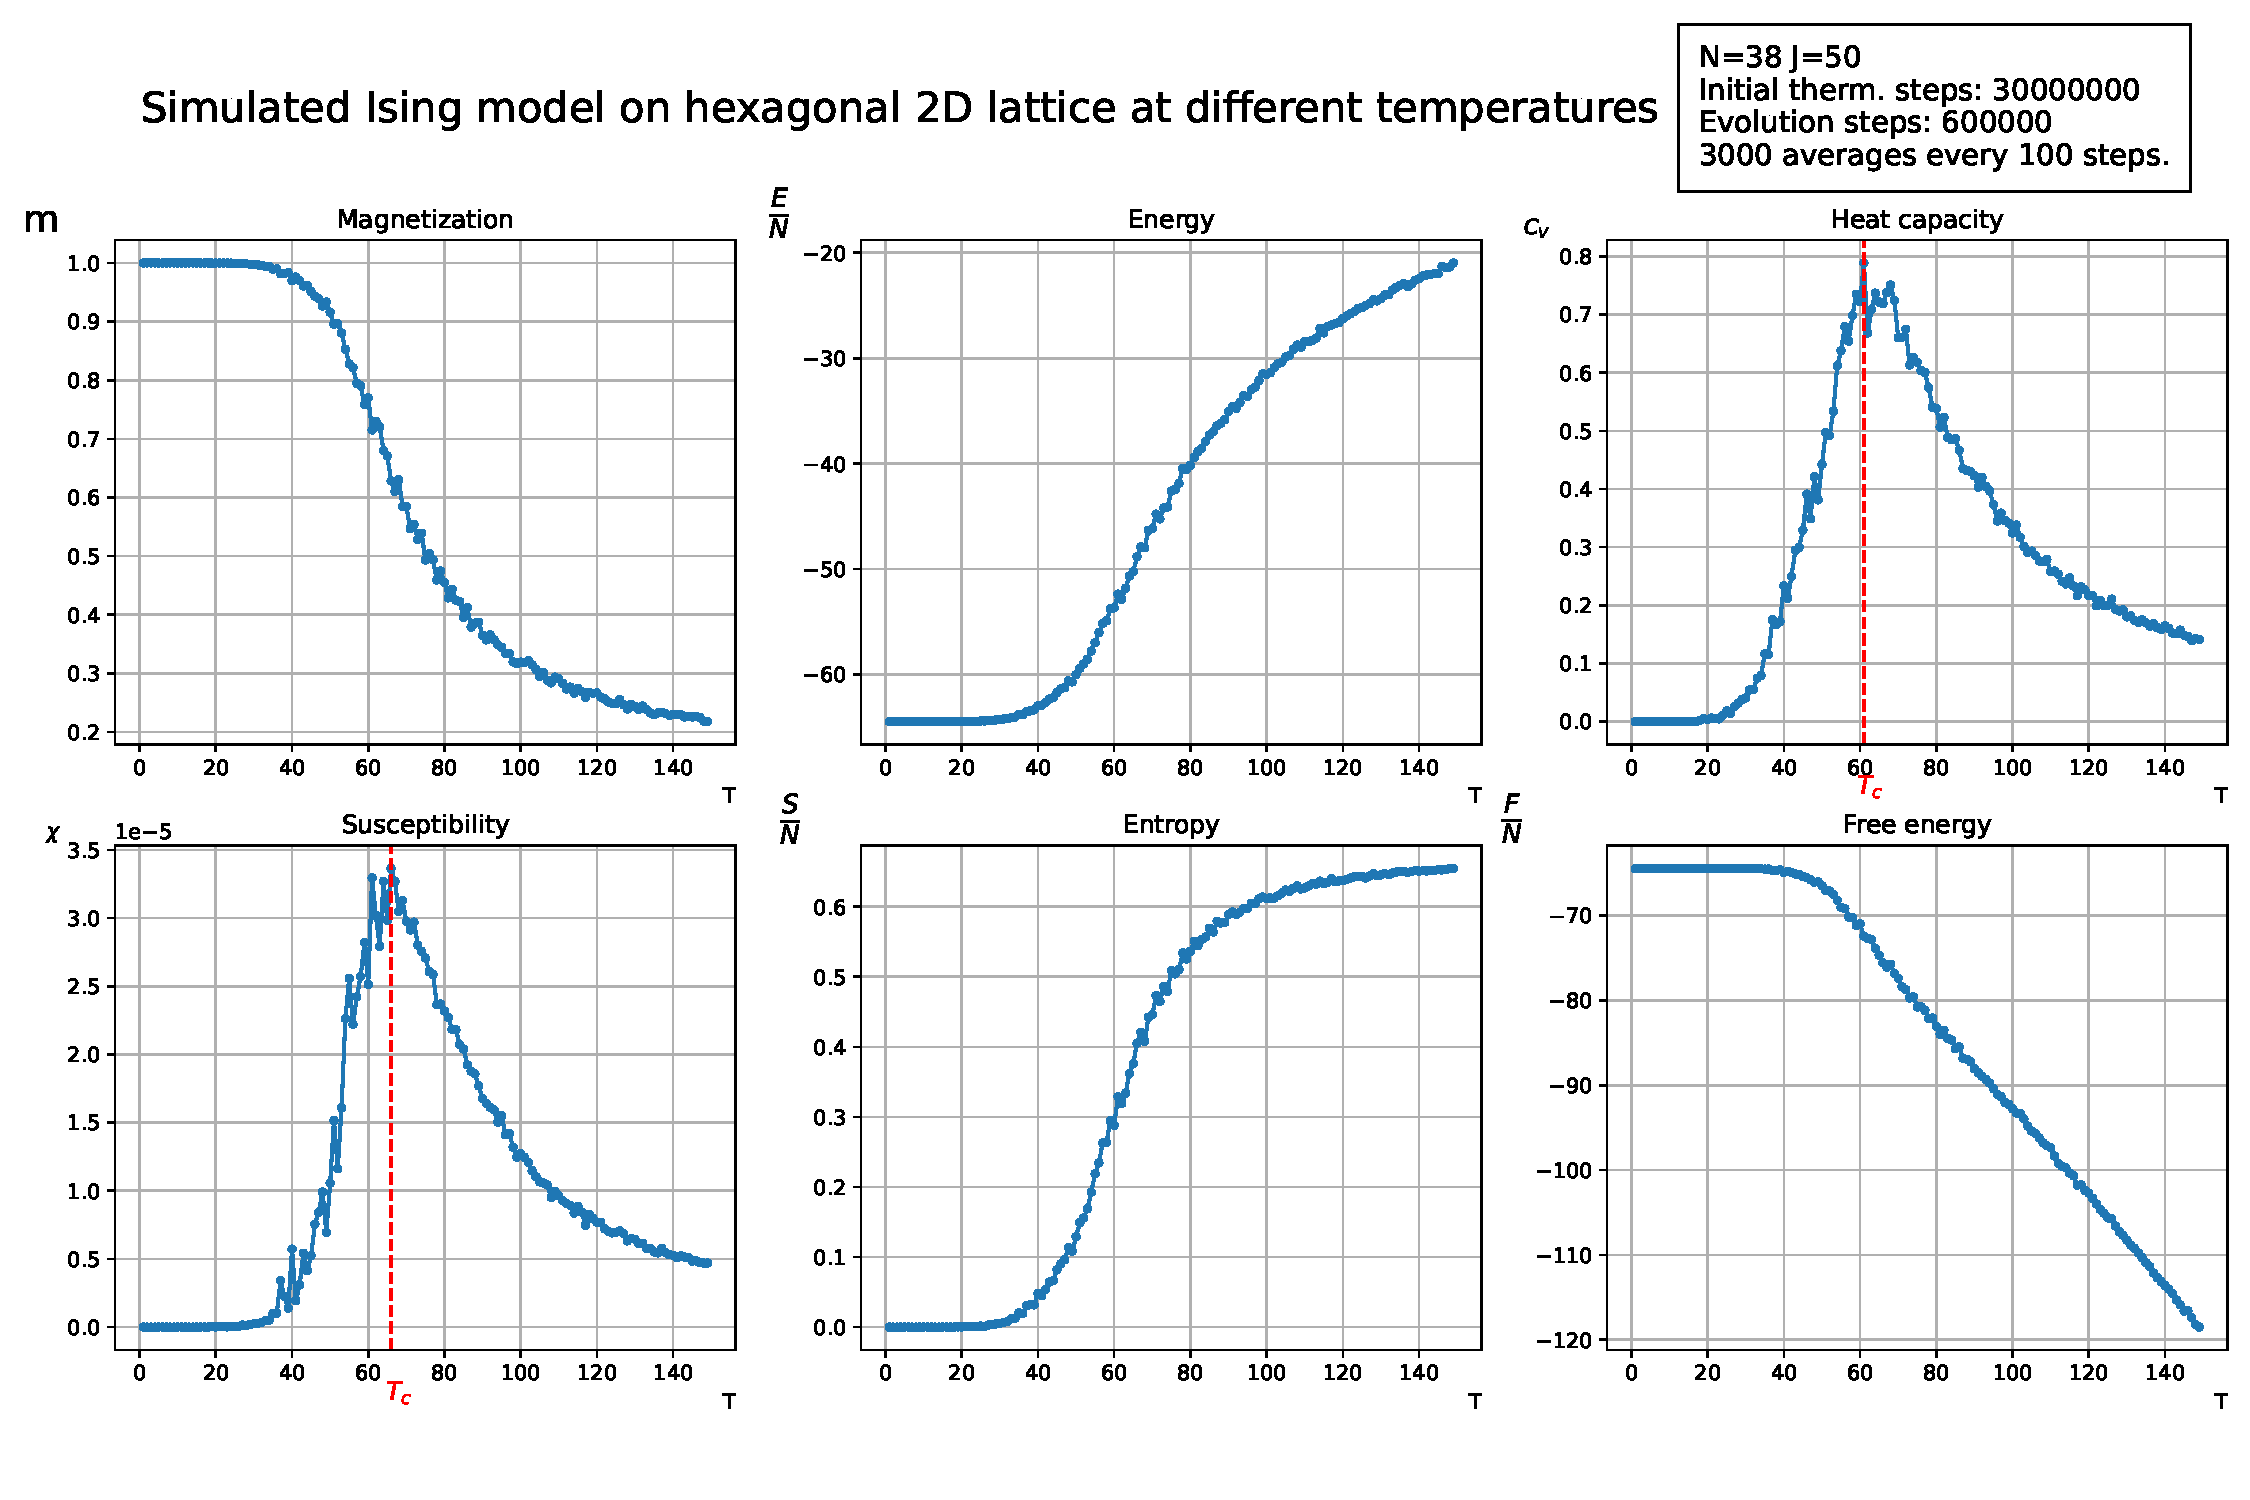
\includegraphics[width=\linewidth]{2d_hexagonal_thermal.pdf}
      \caption{Behavior of the hexagonal lattice at increasing temperatures. We highlighted with a dashed line the critical temperatures we measured.}\label{Fig:Behaviour3}
\end{figure}
We plotted the absolute value of the magnetization (to have a more readable plot), we can see that at low temperatures $m$ is close to 1, and then it quickly transitions to a zero magnetization around the critical temperature. Also the entropy, at the critical temperature, transitions from 0 to higher value, as we expected transitioning from ordered states to disordered ones. The heat capacity and the susceptibility also show the phase transition since, as expected, they have a peak around the critical temperatures. Lastly, the energy is constant at low temperatures and then, while transitioning, it increases, instead the free energy has the opposite behavior.

For each lattice we determined the phase transition temperature using the peak of the susceptibility and the heat capacity (which should diverge at $T=T_c$), then we compared the results with the theoretical predictions we previously discussed.
\begin{table}[!htbp]
    \centering
    \label{Tab:Check}
    \begin{tabular}{cccc}
        \toprule
        \multirow{2}{*}{Lattice} & \multicolumn{3}{c}{Critical temperature} \\
         \cmidrule(lr){2-4}
        & $C_V$ measure &  $\chi$ measure & Theoretical \\
        \midrule
        2D Square $30\times30$ & $1.11\times10^{2}$ & $1.13\times10^{2}$ & $1.134645\times10^{2}$ \\
        2D Triangular $30\times30$ & $1.78\times10^{2}$ & $1.77\times10^{2}$ & $1.82048\times10^{2}$ \\
        2D Hexagonal $4\times3$ & $6.1\times10^1$ & $6.6\times10^1$ & $7.5\times10^1$ \\
        \bottomrule
    \end{tabular}
    \caption{Comparison between measured and predicted critical temperatures for different lattices. Every measure was obtained from an ensemble of 3000 system every 100 steps at every $\Delta T=1$ with $J=50$.}
\end{table}

Table \ref{Tab:Check} shows that our model behaves in the predicted way since the measured critical temperatures are in agreement with the exact theoretical one. 

\subsection{The phase transition of the network}
We now want to study the behavior of the network itself as the temperature varies. As we already mentioned, we divided the network into the spin up and spin down networks to study them separately. In this way, when studying how these networks are connected (connected components, connectivity, and so on) we are studying how neighbors aligned atoms group together creating domains. Since the network measures are computationally heavy, we reduced the number of atoms and also the number of points that we measured: the next graphs will show measures repeated every $\Delta T=5$. Let's first analyze the simplest structure, the square lattice.

The first thing that we note in Figure \ref{Fig:squareNetworkmeasure} is that these graphs show really well the spontaneous symmetry breaking behavior, that otherwise only the non-zero magnetization would signal. Indeed, we can see that spin up and spin down networks behave in totally different ways at low temperature: initially all the spins all aligned, and thus they form 1 single connected component. As the temperature raises it starts to appear a second connected component of a few anti-aligned spins until, approaching the critical temperature, we start to get more  connected components and both networks break into smaller components. After the critical temperature the broken symmetry is restored and both networks behave in the same way: the number of components keeps to increase with the temperature while the size of the giant components asymptotically reaches 20 nodes. This shows that at high temperature aligned atoms still form two big connected networks containing almost half of the atoms each (one is spin up while the other spin down) with a few satellites small groups of atoms. However, the betweenness centrality, the diameter of the giant components and the average node connectivity of the giant components show that at higher temperatures the networks become less connected. The raise of the betweenness centrality means that the number of the shortest path that could be broken by removing 1 node increases. This is even better shown by the node connectivity: approaching 1 it signals that removing 1 single node is enough to disconnect the giant components. Lastly, the diameter shows that, even though the giant components are not chains, their structure is close to it: before the critical temperature we observe a single giant component with 50 atoms but with a small diameter of just 7 links, instead after the critical temperature each giant component becomes of around 20 atoms but with a higher diameter of almost 10 links. Lastly, we can observe that the density of links (the percentage of links of each network that exist over the possible ones) has a spike around the critical temperature.

\begin{figure}[!htb]
  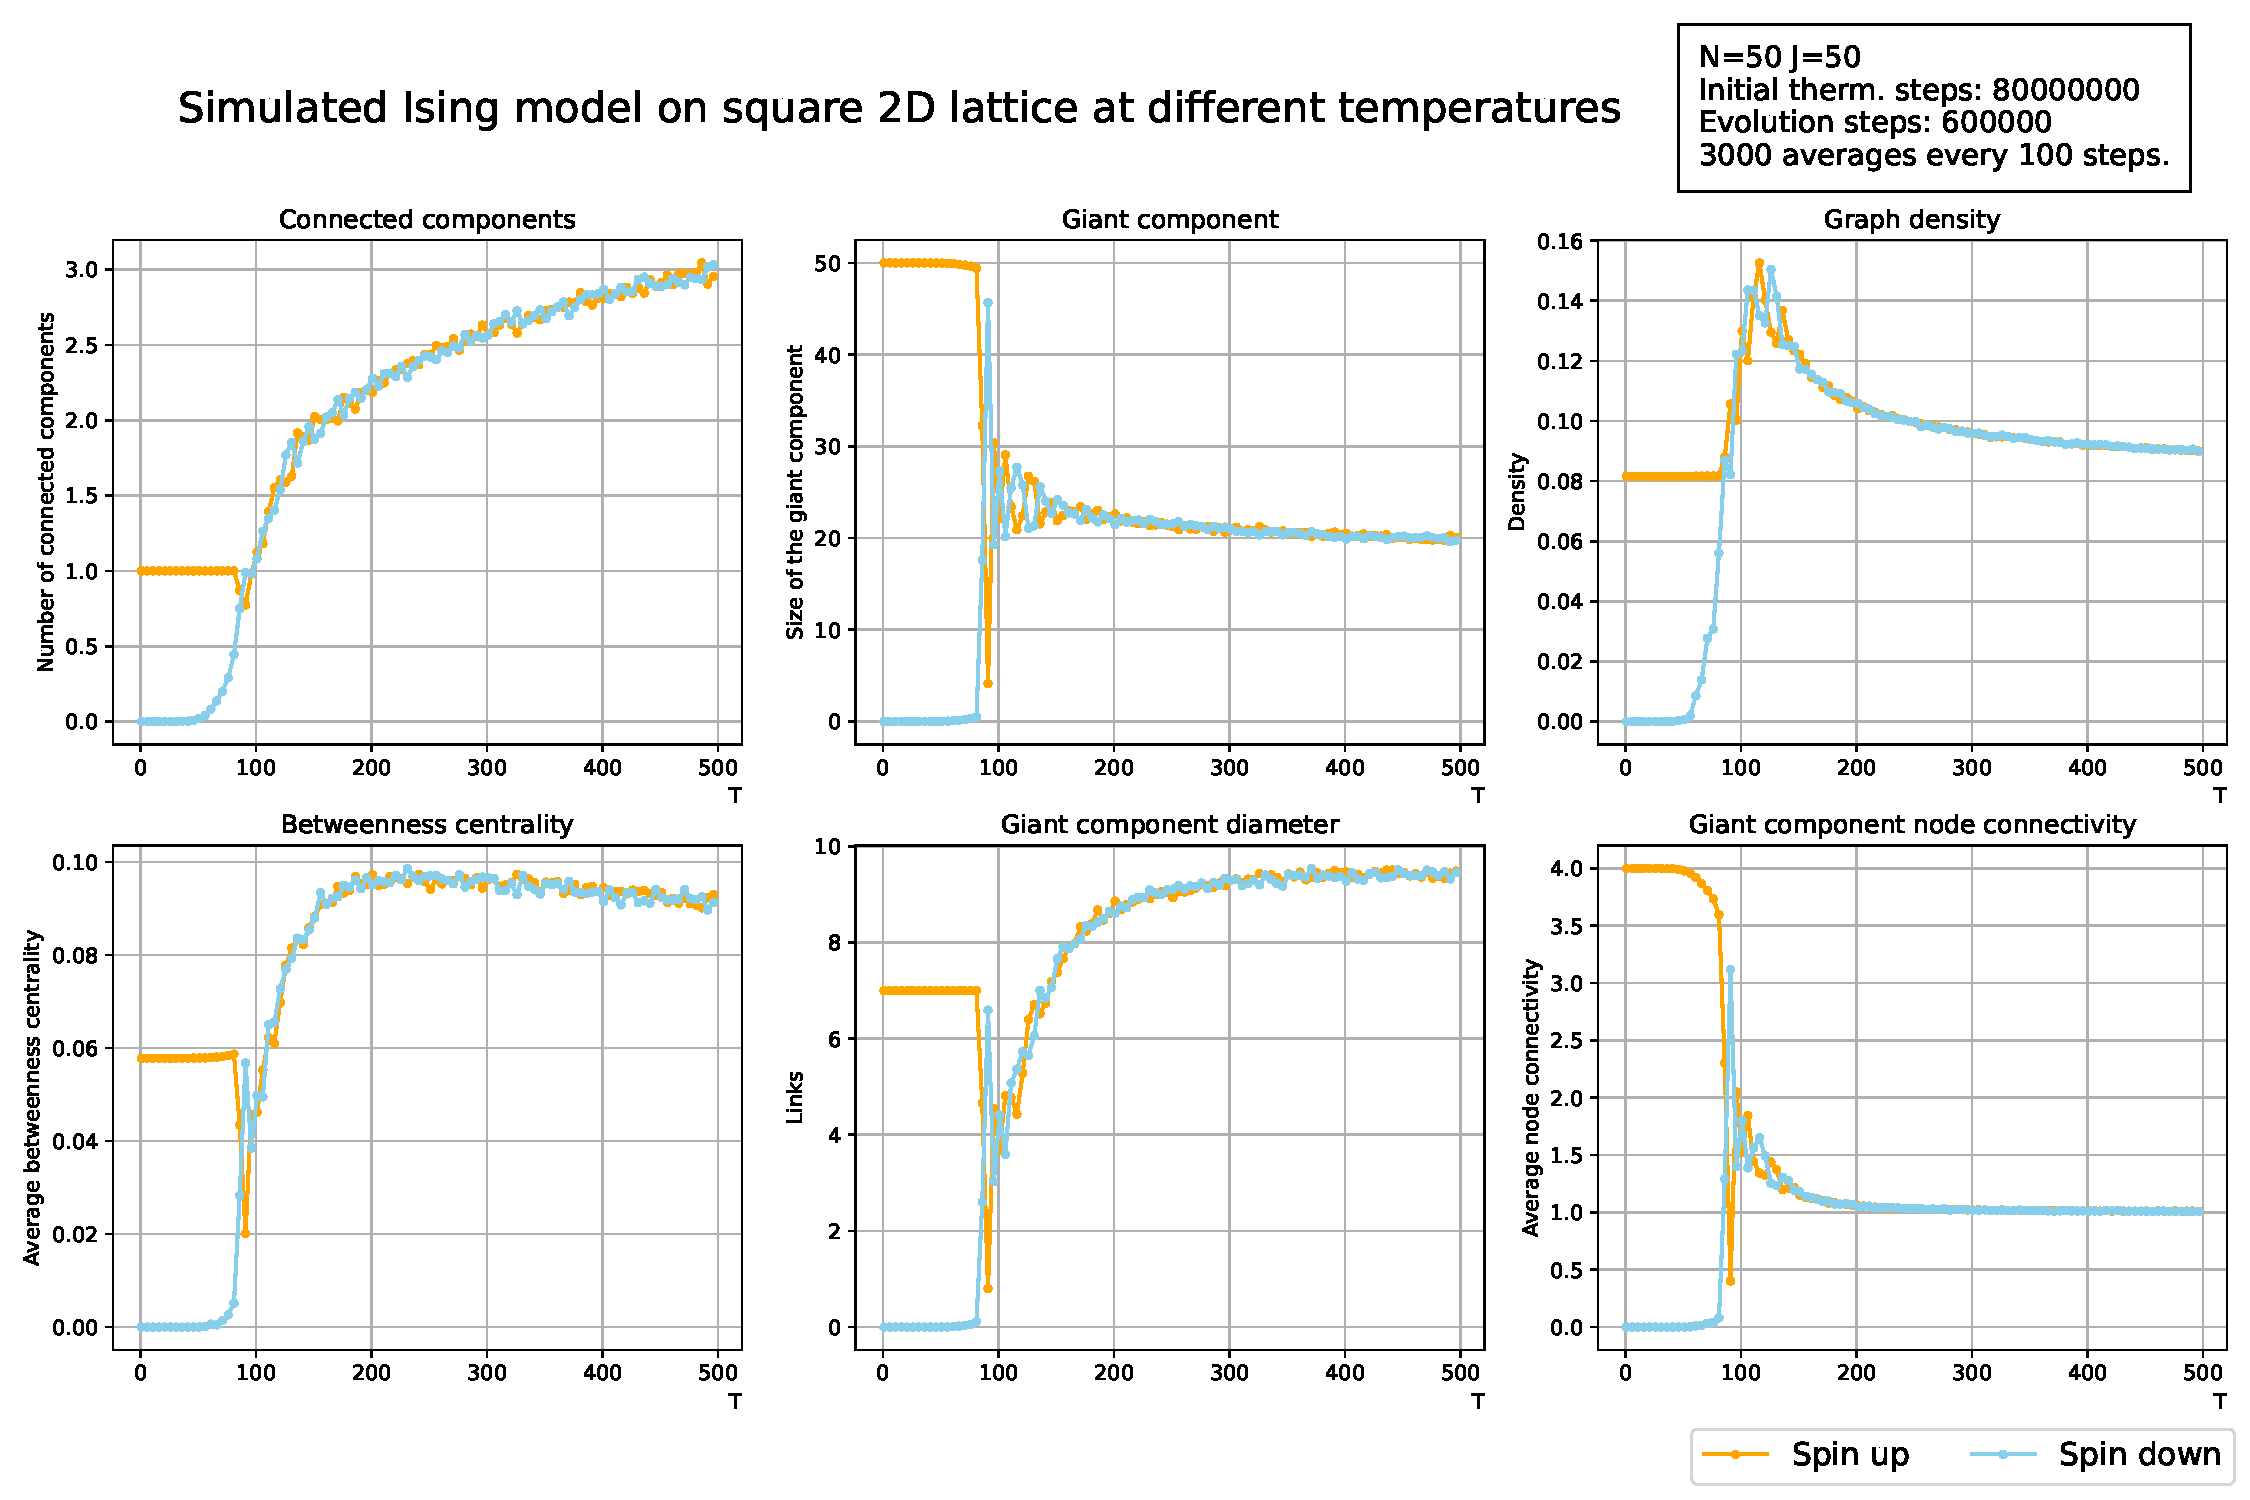
\includegraphics[width=\linewidth]{Network meausres/Square_Network.pdf}
    \caption{Behavior of the network proprieties of the square lattice at increasing temperatures. The orange line is the spin up network while the blue is the spin down one.}
    \label{Fig:squareNetworkmeasure}
\end{figure}

\begin{figure}[!htb]
  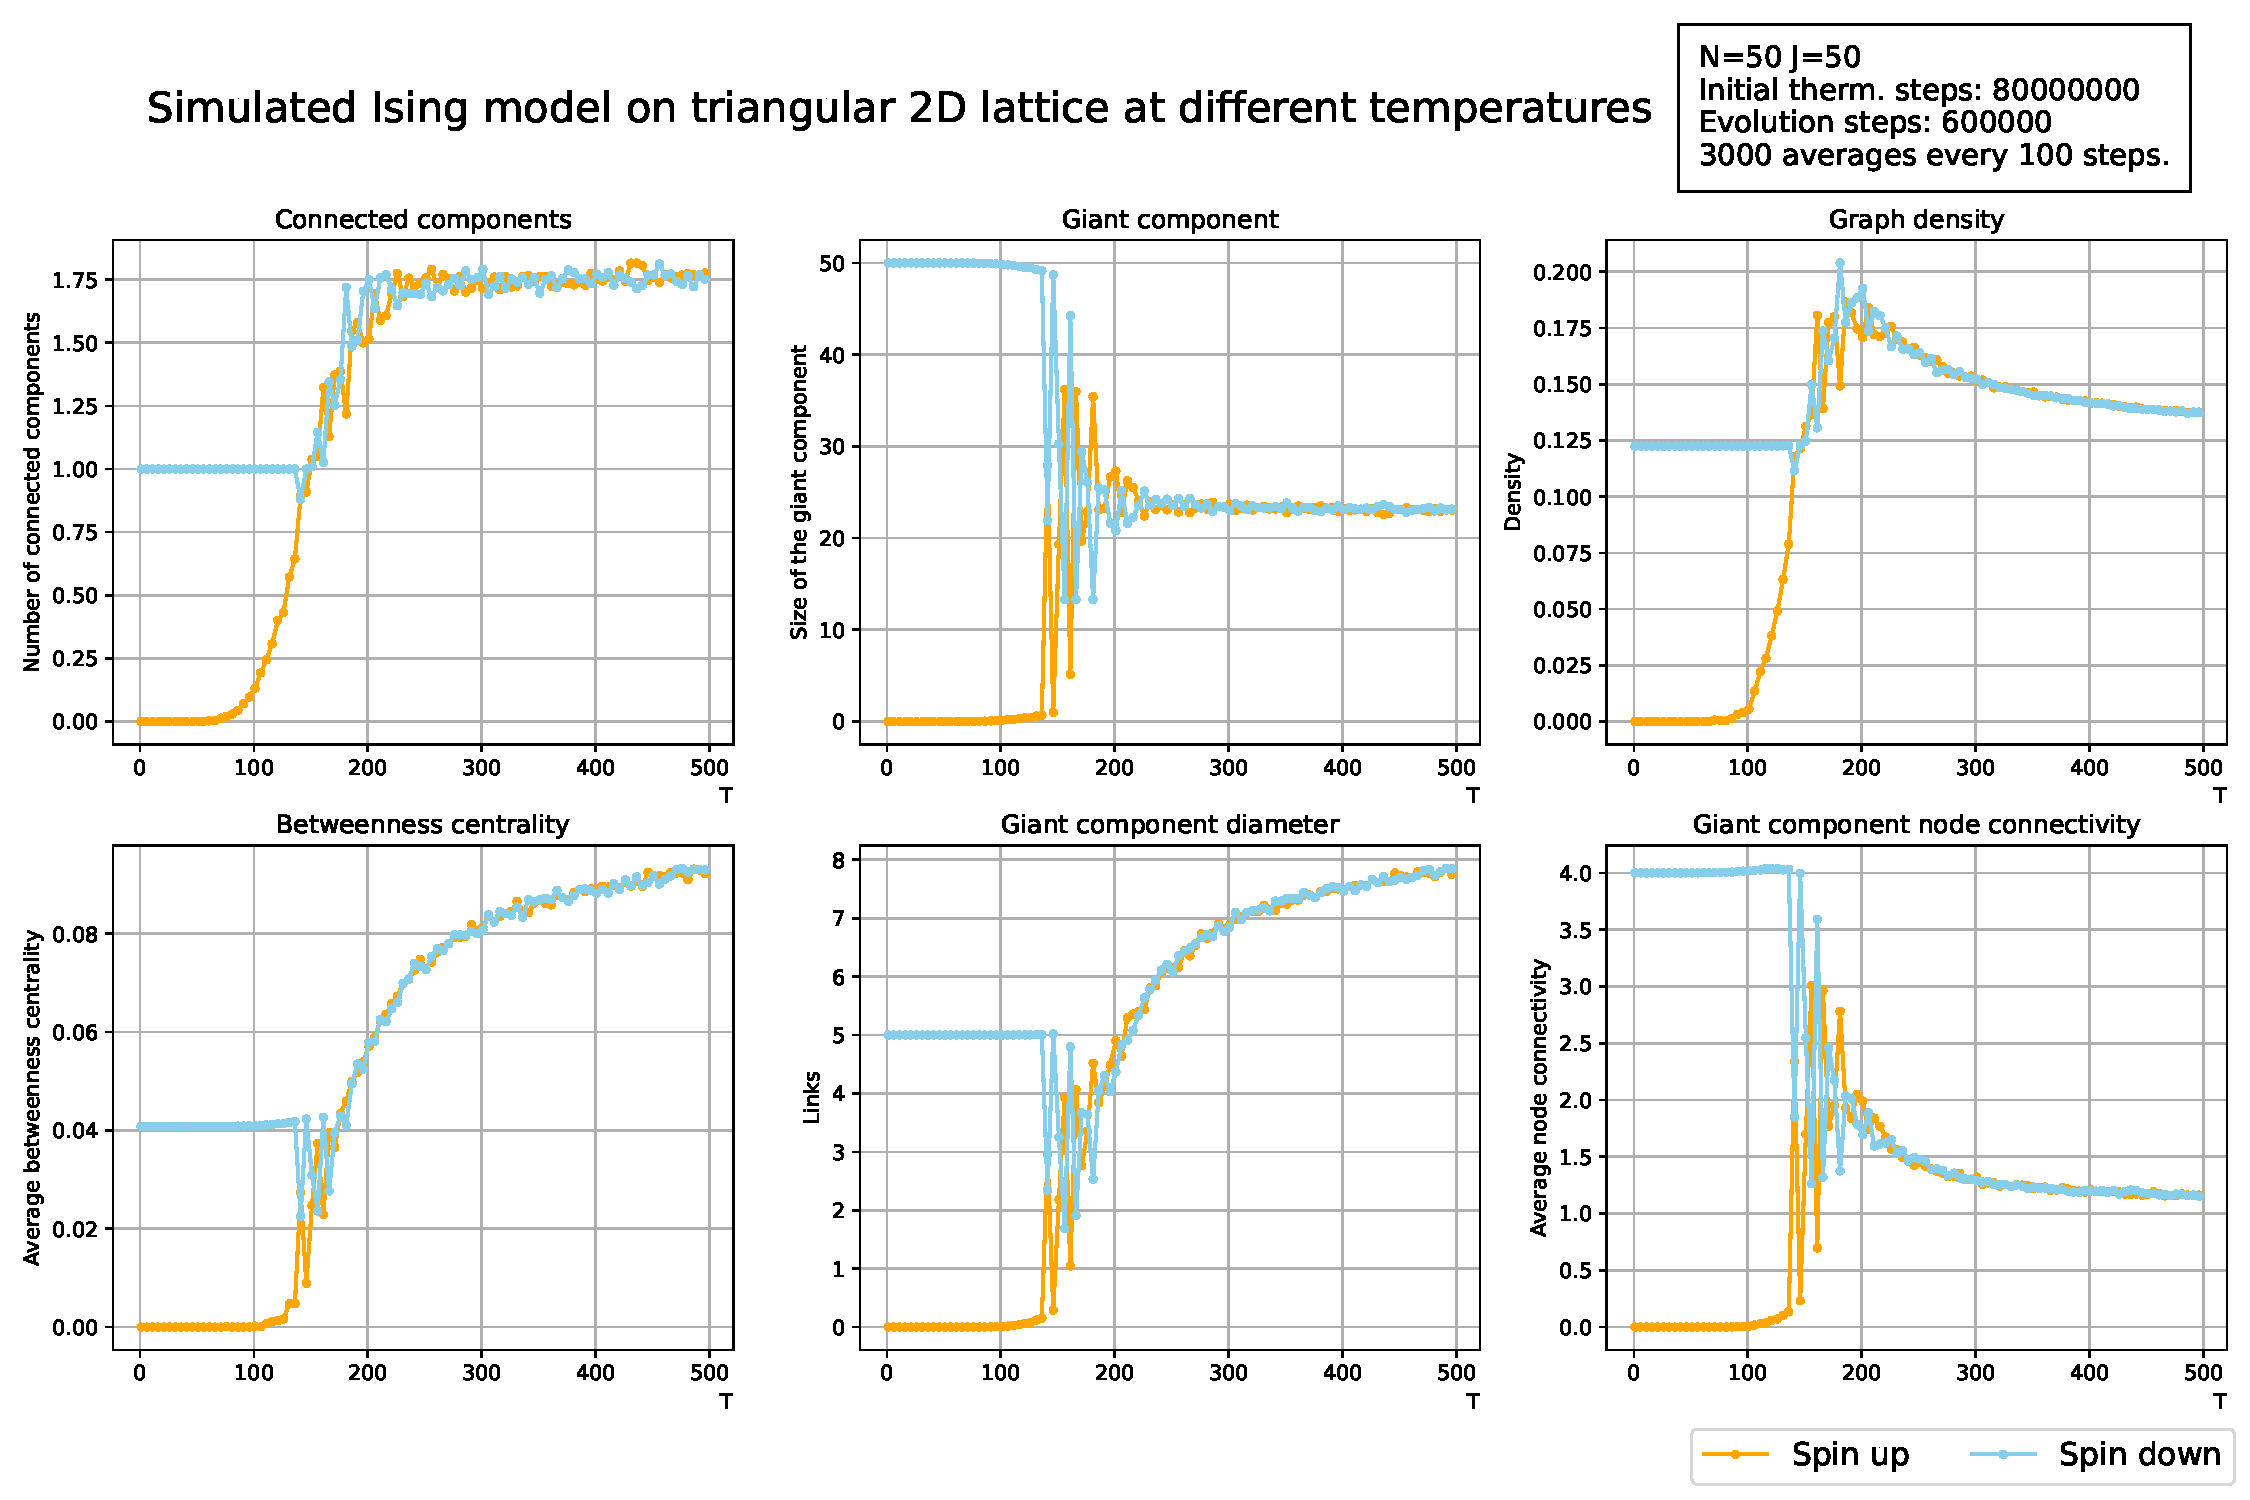
\includegraphics[width=.96\linewidth]{Network meausres/Triangular_Network.pdf}
    \caption{Behavior of the network proprieties of the triangular lattice at increasing temperatures. The orange line is the spin up network while the blue is the spin down one.}
    \label{Fig:triangularNetworkmeasure}
\end{figure}

\begin{figure}[!htb]
  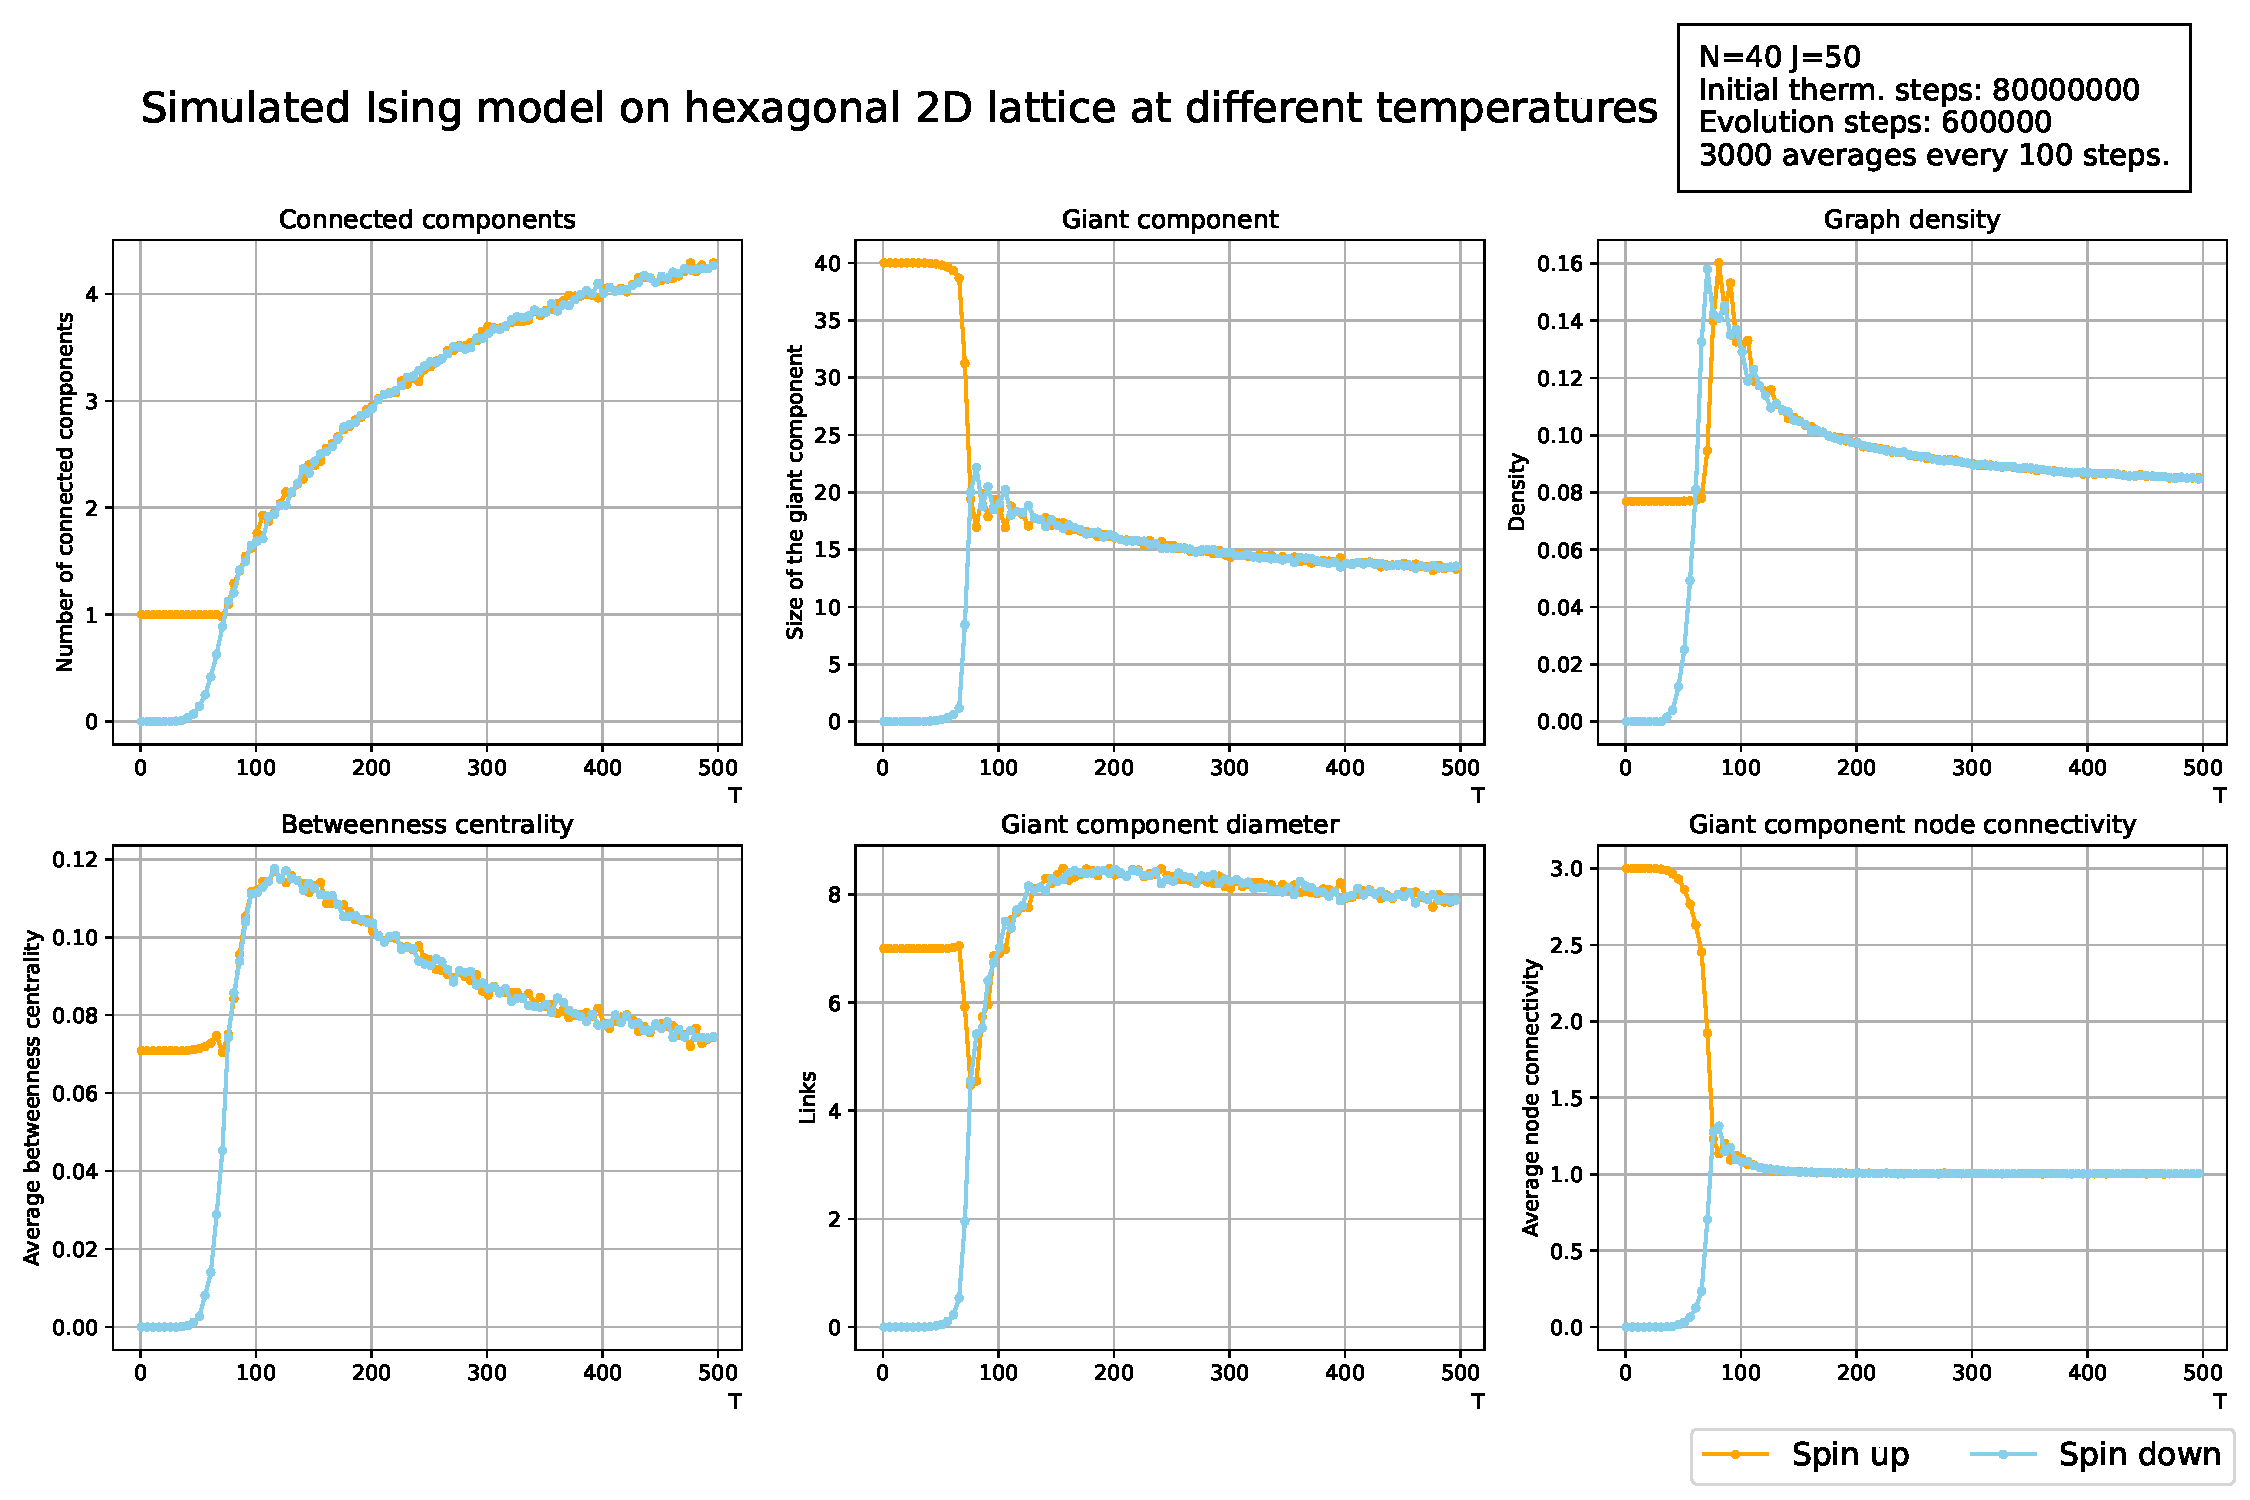
\includegraphics[width=.96\linewidth]{Network meausres/Hexagonal_Network.pdf}
    \caption{Behavior of the network proprieties of the hexagonal lattice at increasing temperatures. The orange line is the spin up network while the blue is the spin down one.}
    \label{Fig:hexagonalNetworkmeasure}
\end{figure}

Also the triangular and hexagonal lattices show the features we have just described. Figure \ref{Fig:triangularNetworkmeasure} shows that the triangular lattice breaks into fewer connected components with a slightly bigger giant compoents. Figure \ref{Fig:hexagonalNetworkmeasure} instead shows that hexagonal lattices break in more connected components, over 4, generating smaller giant components, with almost a third of atoms each. Furthermore, the hexagonal lattice shows an interesting behavior of the betweenness centrality: at the critical temperature it reaches a maximum point. This can be interpreted in the following way: first the network breaks into smaller components of a few atoms each with a higher betweenness centrality, however, then these smaller components start to become bigger and more connected and therefore their betweenness centrality drops.

\begin{figure}[!htb]
  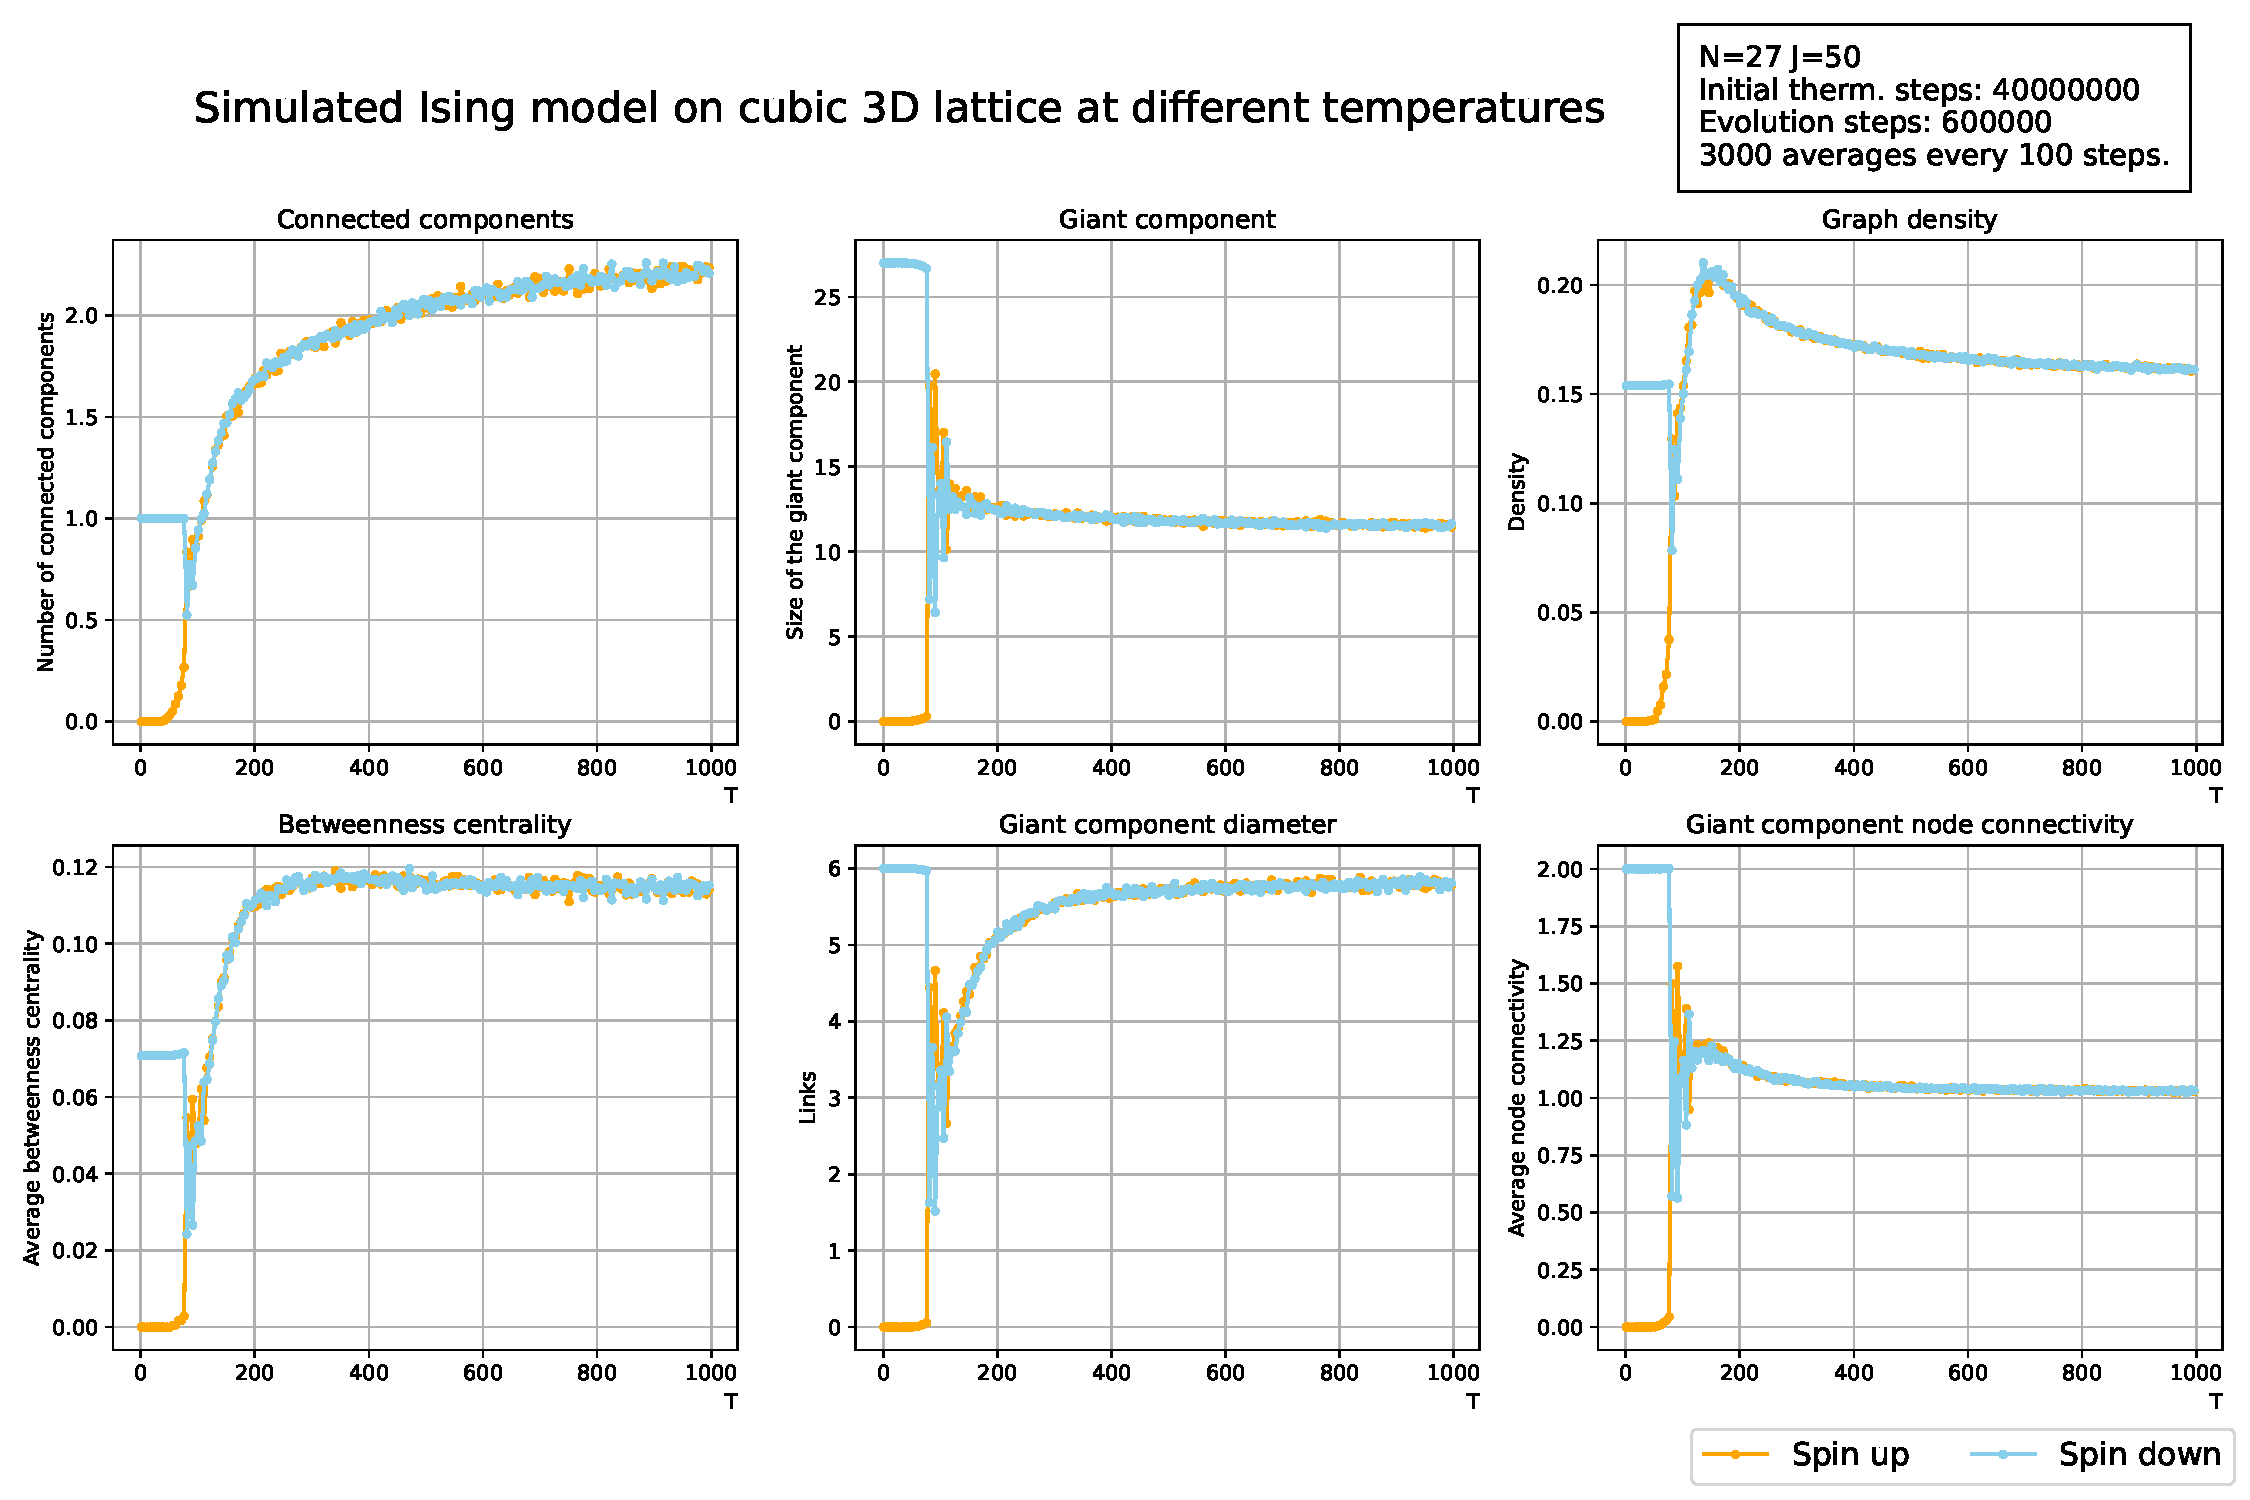
\includegraphics[width=\linewidth]{Network meausres/3D_Network.pdf}
    \caption{Behavior of the network proprieties of the 3D cubic lattice at increasing temperatures. The orange line is the spin up network while the blue is the spin down one.}
    \label{Fig:3DNetworkmeasure}
\end{figure}

The last analysis we conducted is on the 3D cubic lattice: this is shown in Figure \ref{Fig:3DNetworkmeasure}. The same behavior of the previous networks is again showed by the 3D cubic lattice, however it is interesting to note that in this case the diameter of the giant component, after its drop during the phase transition, slowly rises again approaching $6$ links, which is the diameter of the all aligned lattice at $T=0$.

Another interesting observation that emerges from these graphs is that, even though we analyzed 4 different types of networks in different dimension, staring from different average node connectivity all converges to 1 after the phase transition. This shows that, independently of the network proprieties, all aligned spins networks become a tree graph. 

\subsection{Exotic networks}
In this last section we will analyze some exotic kind of networks that we tried to simulate.
\subsubsection*{Broken lattices}
Networks with some fraction of atoms removed (broken) could mimic the behavior of lattices with defects: for this reason we simulated a square lattice of 100 atoms from which we started to remove some fractions of atoms. Form Figure \ref{Fig:BSNetworkmeasure} we can see that as we increase the number of removed atoms the phase transition is still manifest, however the critical temperature starts to change: with only 5 atoms removed the giant component starts to break at around $T=100$ while with 30 atoms removed it happens just after $T=50$. This is not unexpected, since removing atoms we also decrease the number of interactions, from the mean field approximation critical temperature $T_C=JZ$, we can see that lowering the number of links we decrease the critical temperature. Another interesting behavior we observe is that after the phase transition, as we remove atoms, the number of connected component raises: in every simulation we start 1 connected component but then we are left at $T=200$ with around 4 connected components per spin type, for lattices with fewer removed atoms, to over 7 components after the removal of one third of the atoms. As we could expect the size of the giant components get lowered, almost halved. This indicates that as we add defects the atoms struggle more to create magnetic domains. Lastly we observed, during the simulation, that the thermalization time, as we increase the number of removed atoms, increased too. For this reason we could just remove up to 30 atoms.
\begin{figure}[!htb]
\end{figure}
\begin{figure}[!htb]
  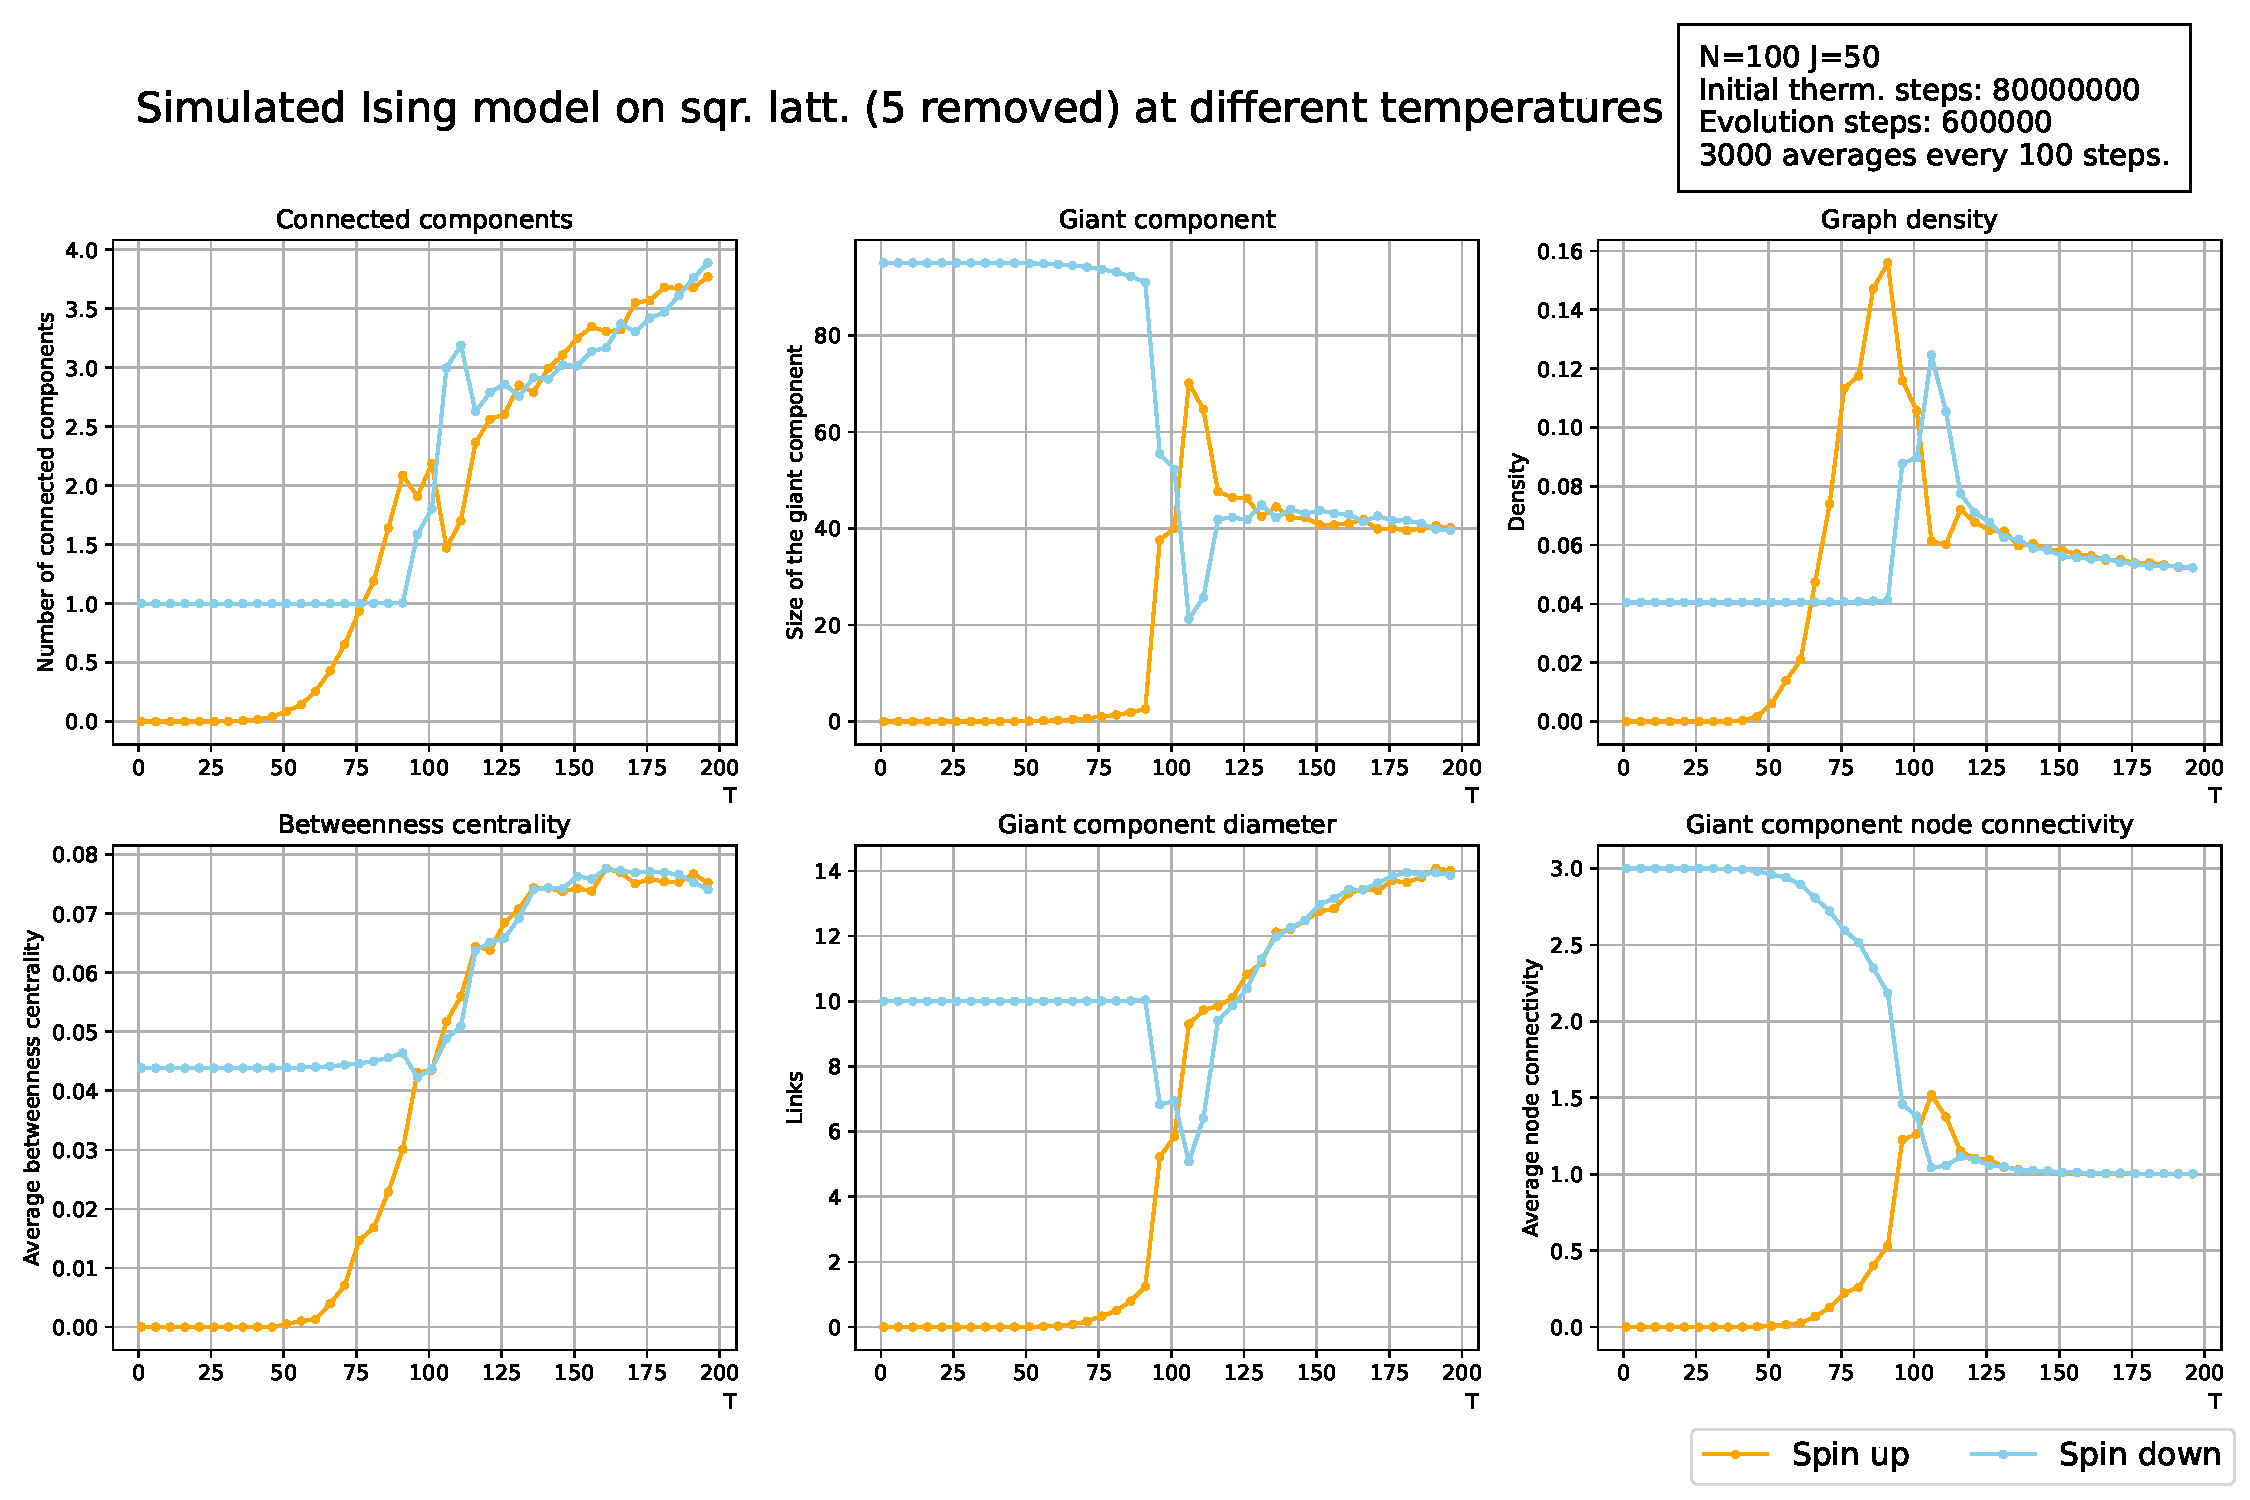
\includegraphics[width=.5\linewidth]{Broken/Figure_5.pdf}
  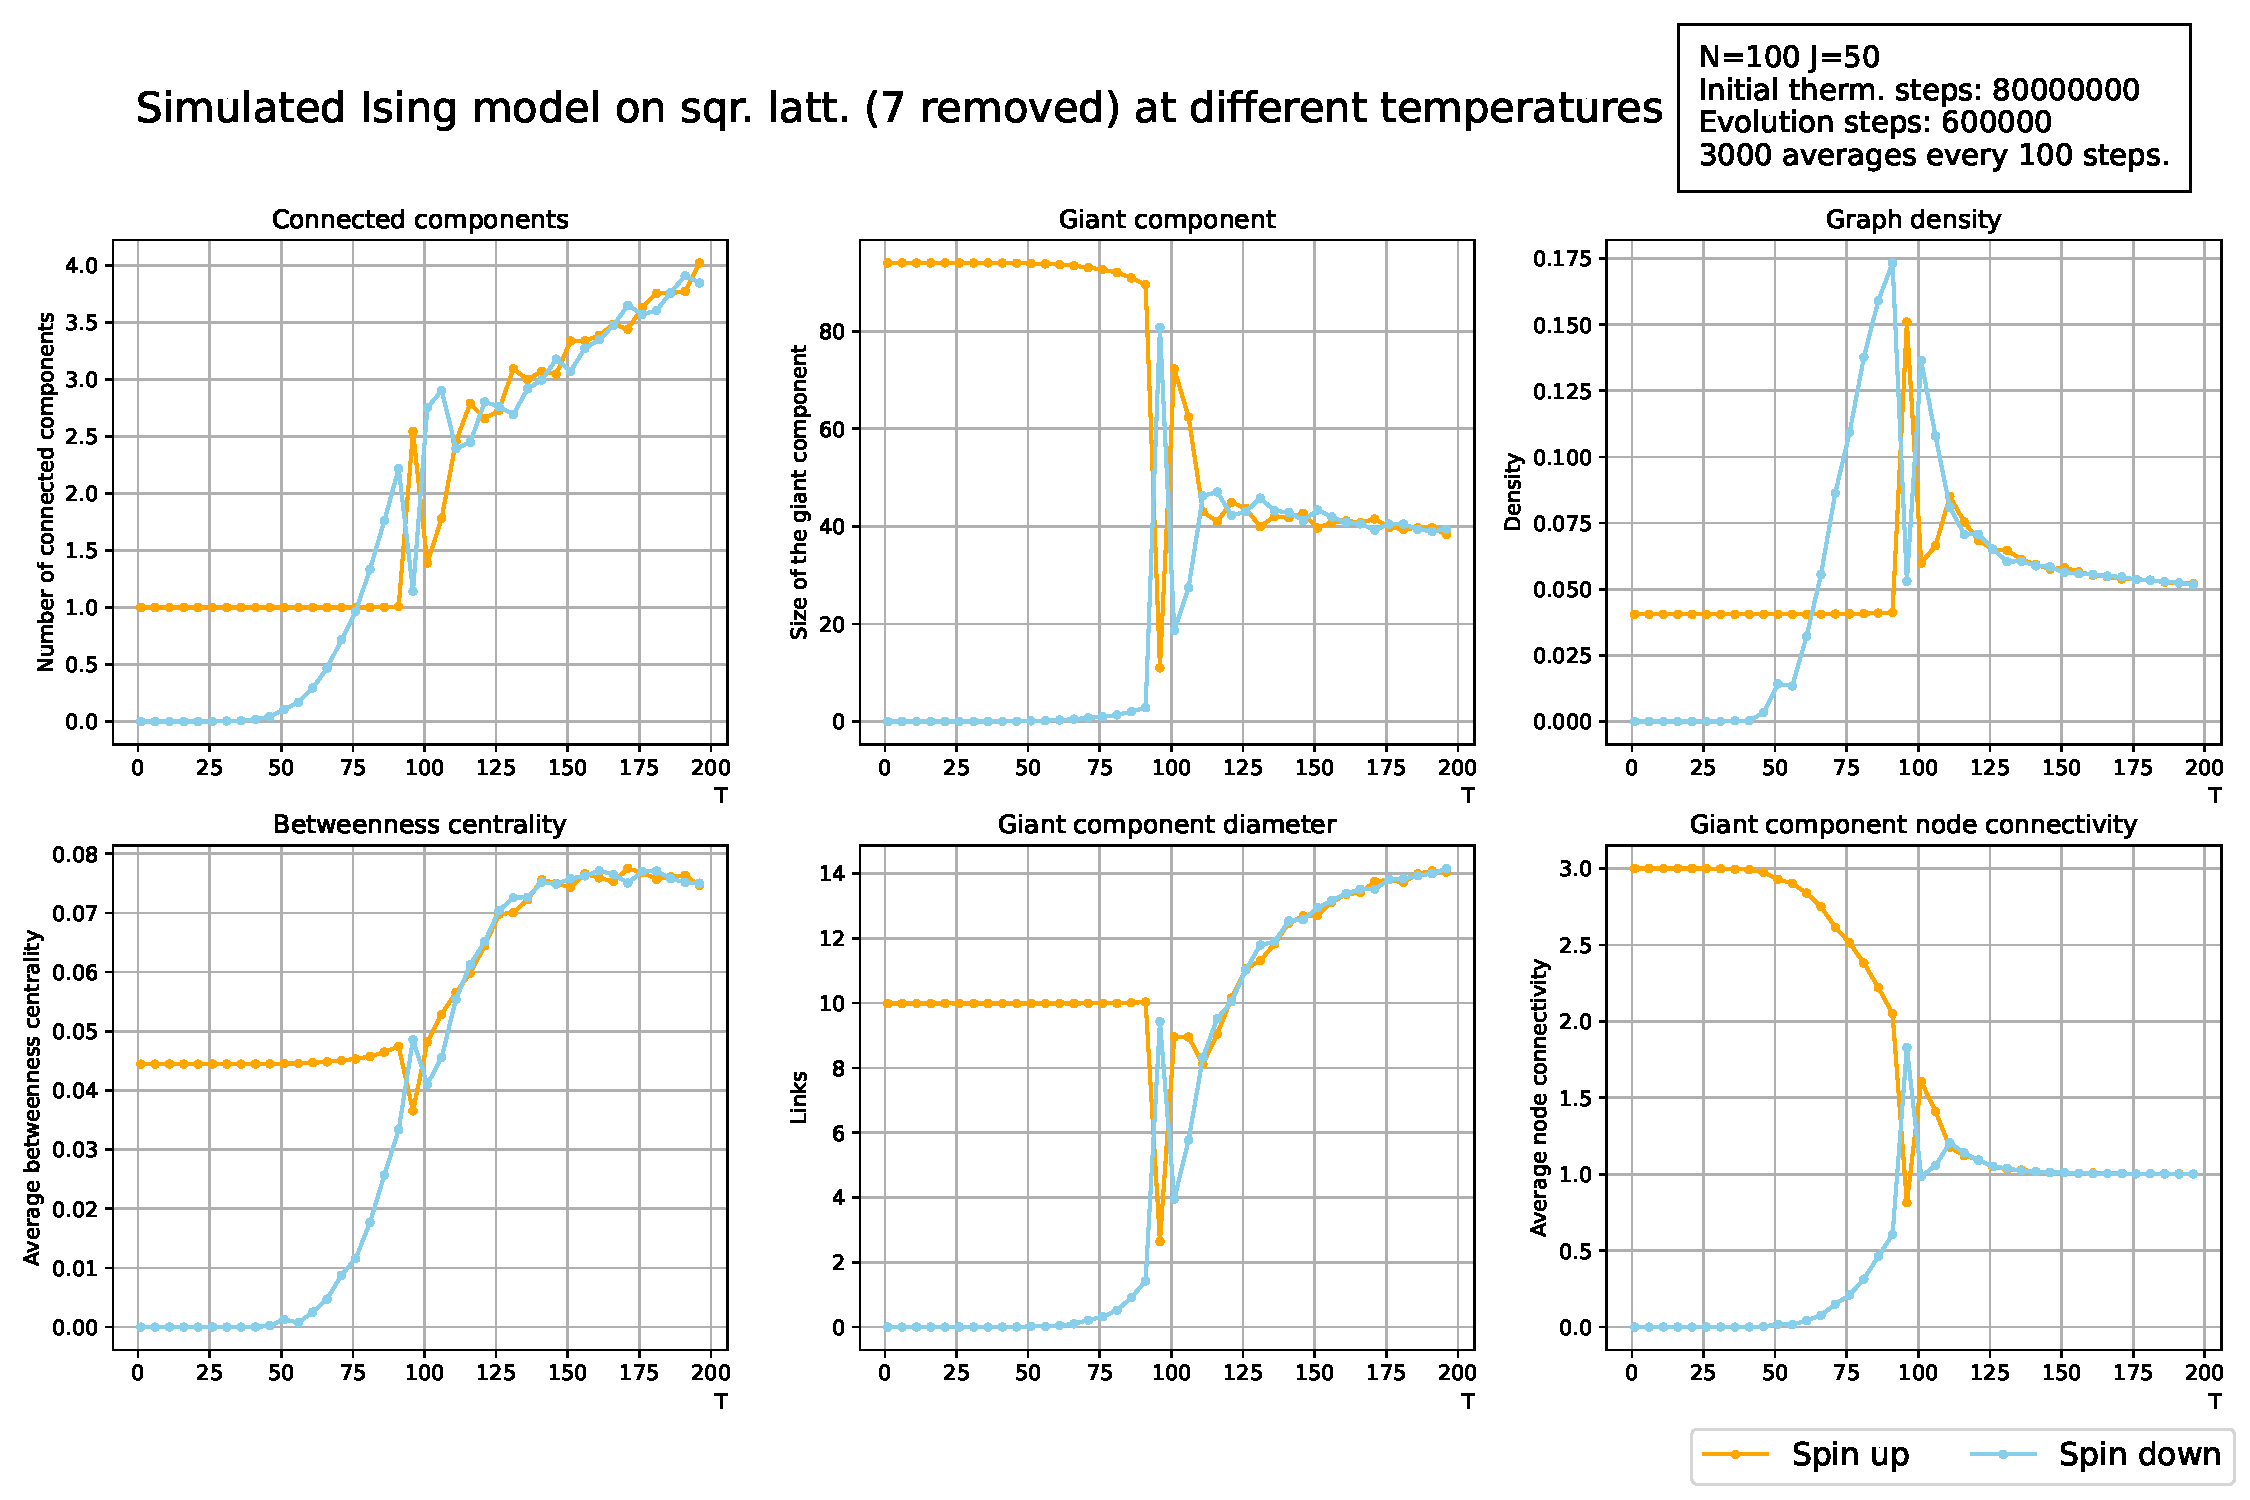
\includegraphics[width=.5\linewidth]{Broken/Square_7.pdf}

  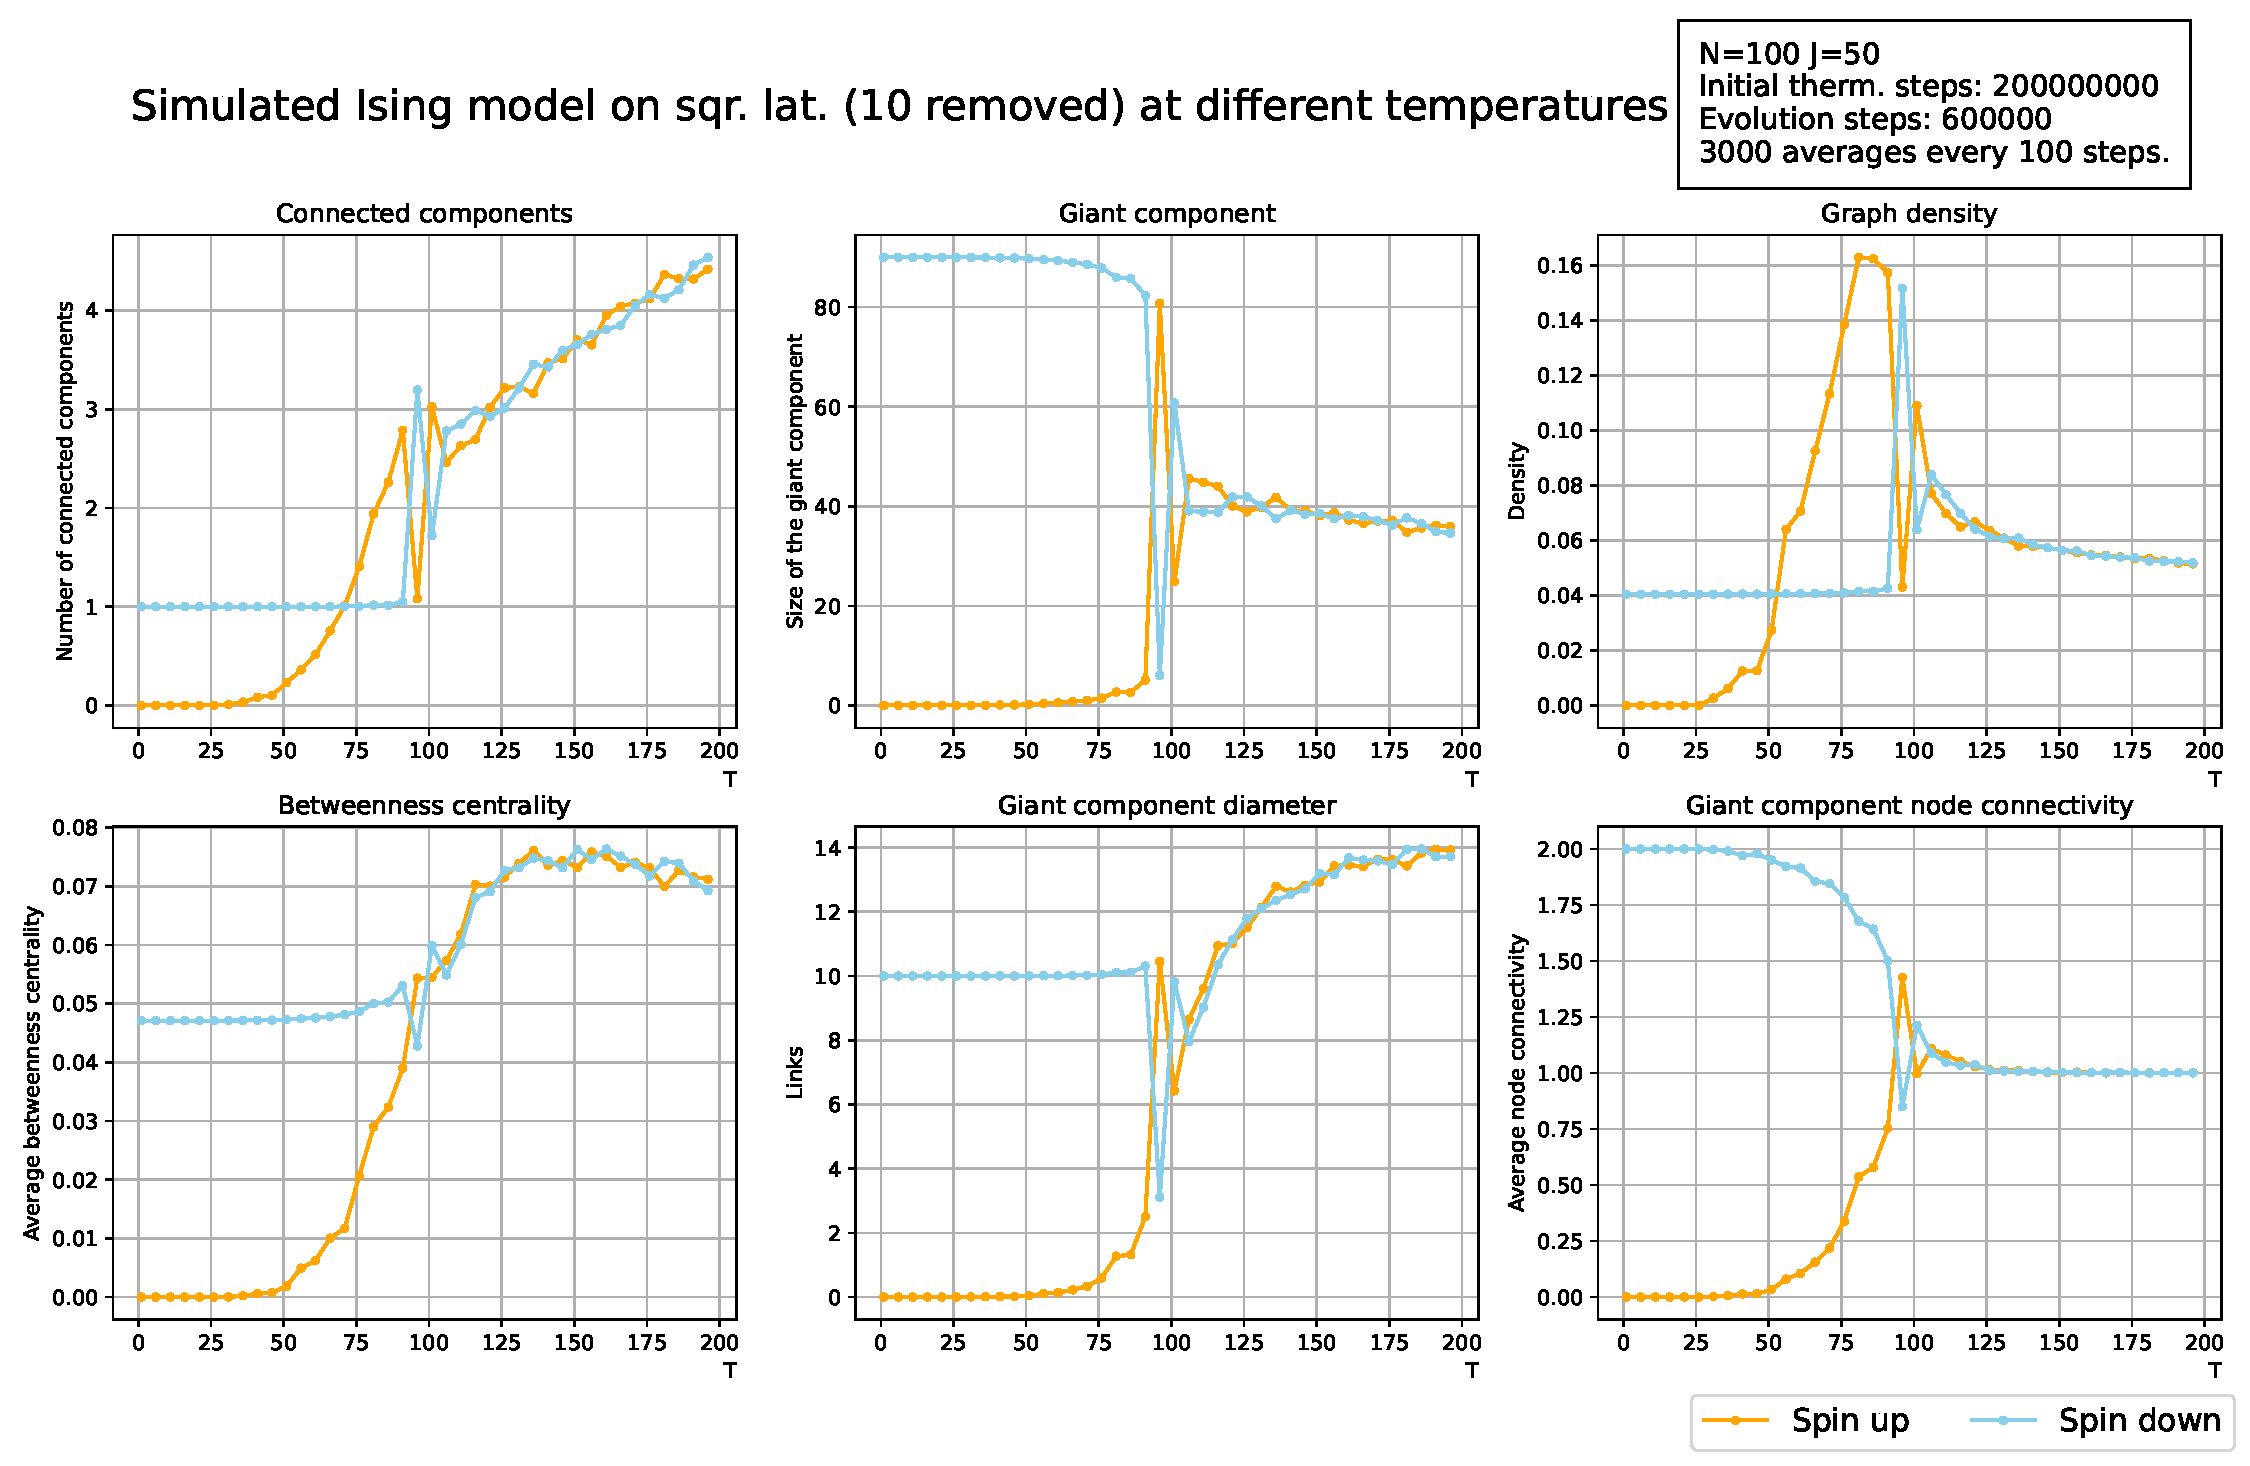
\includegraphics[width=.5\linewidth]{Broken/Square_10.pdf}
  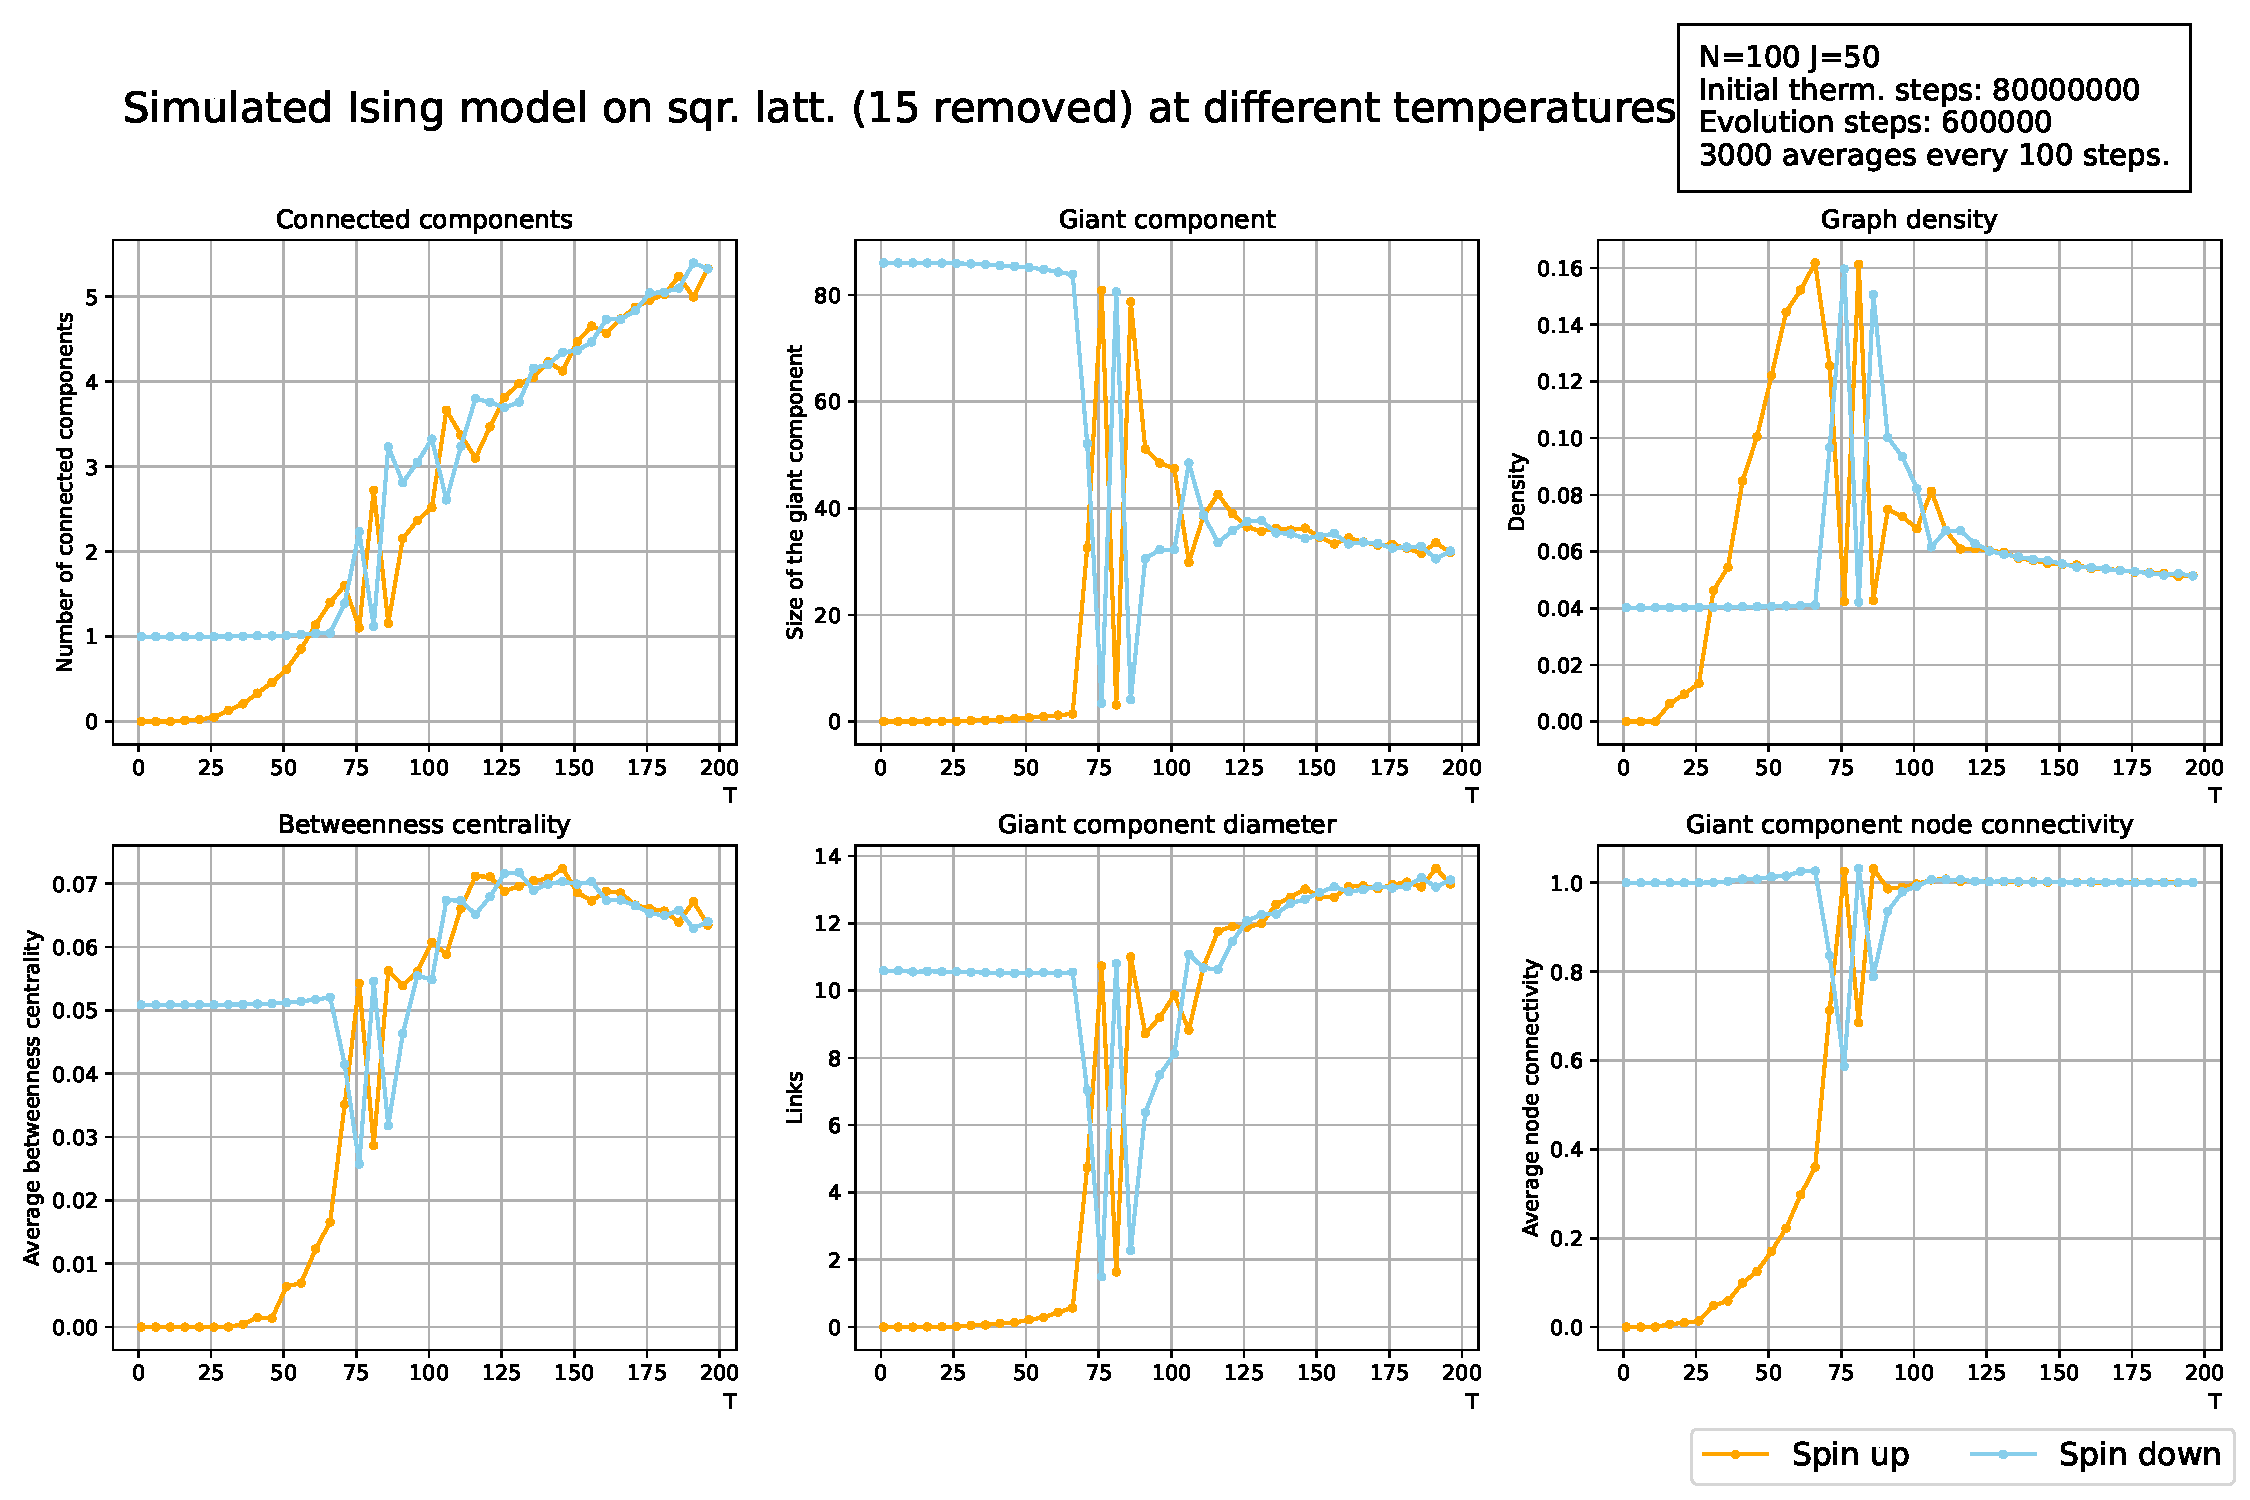
\includegraphics[width=.5\linewidth]{Broken/Square_15.pdf}

  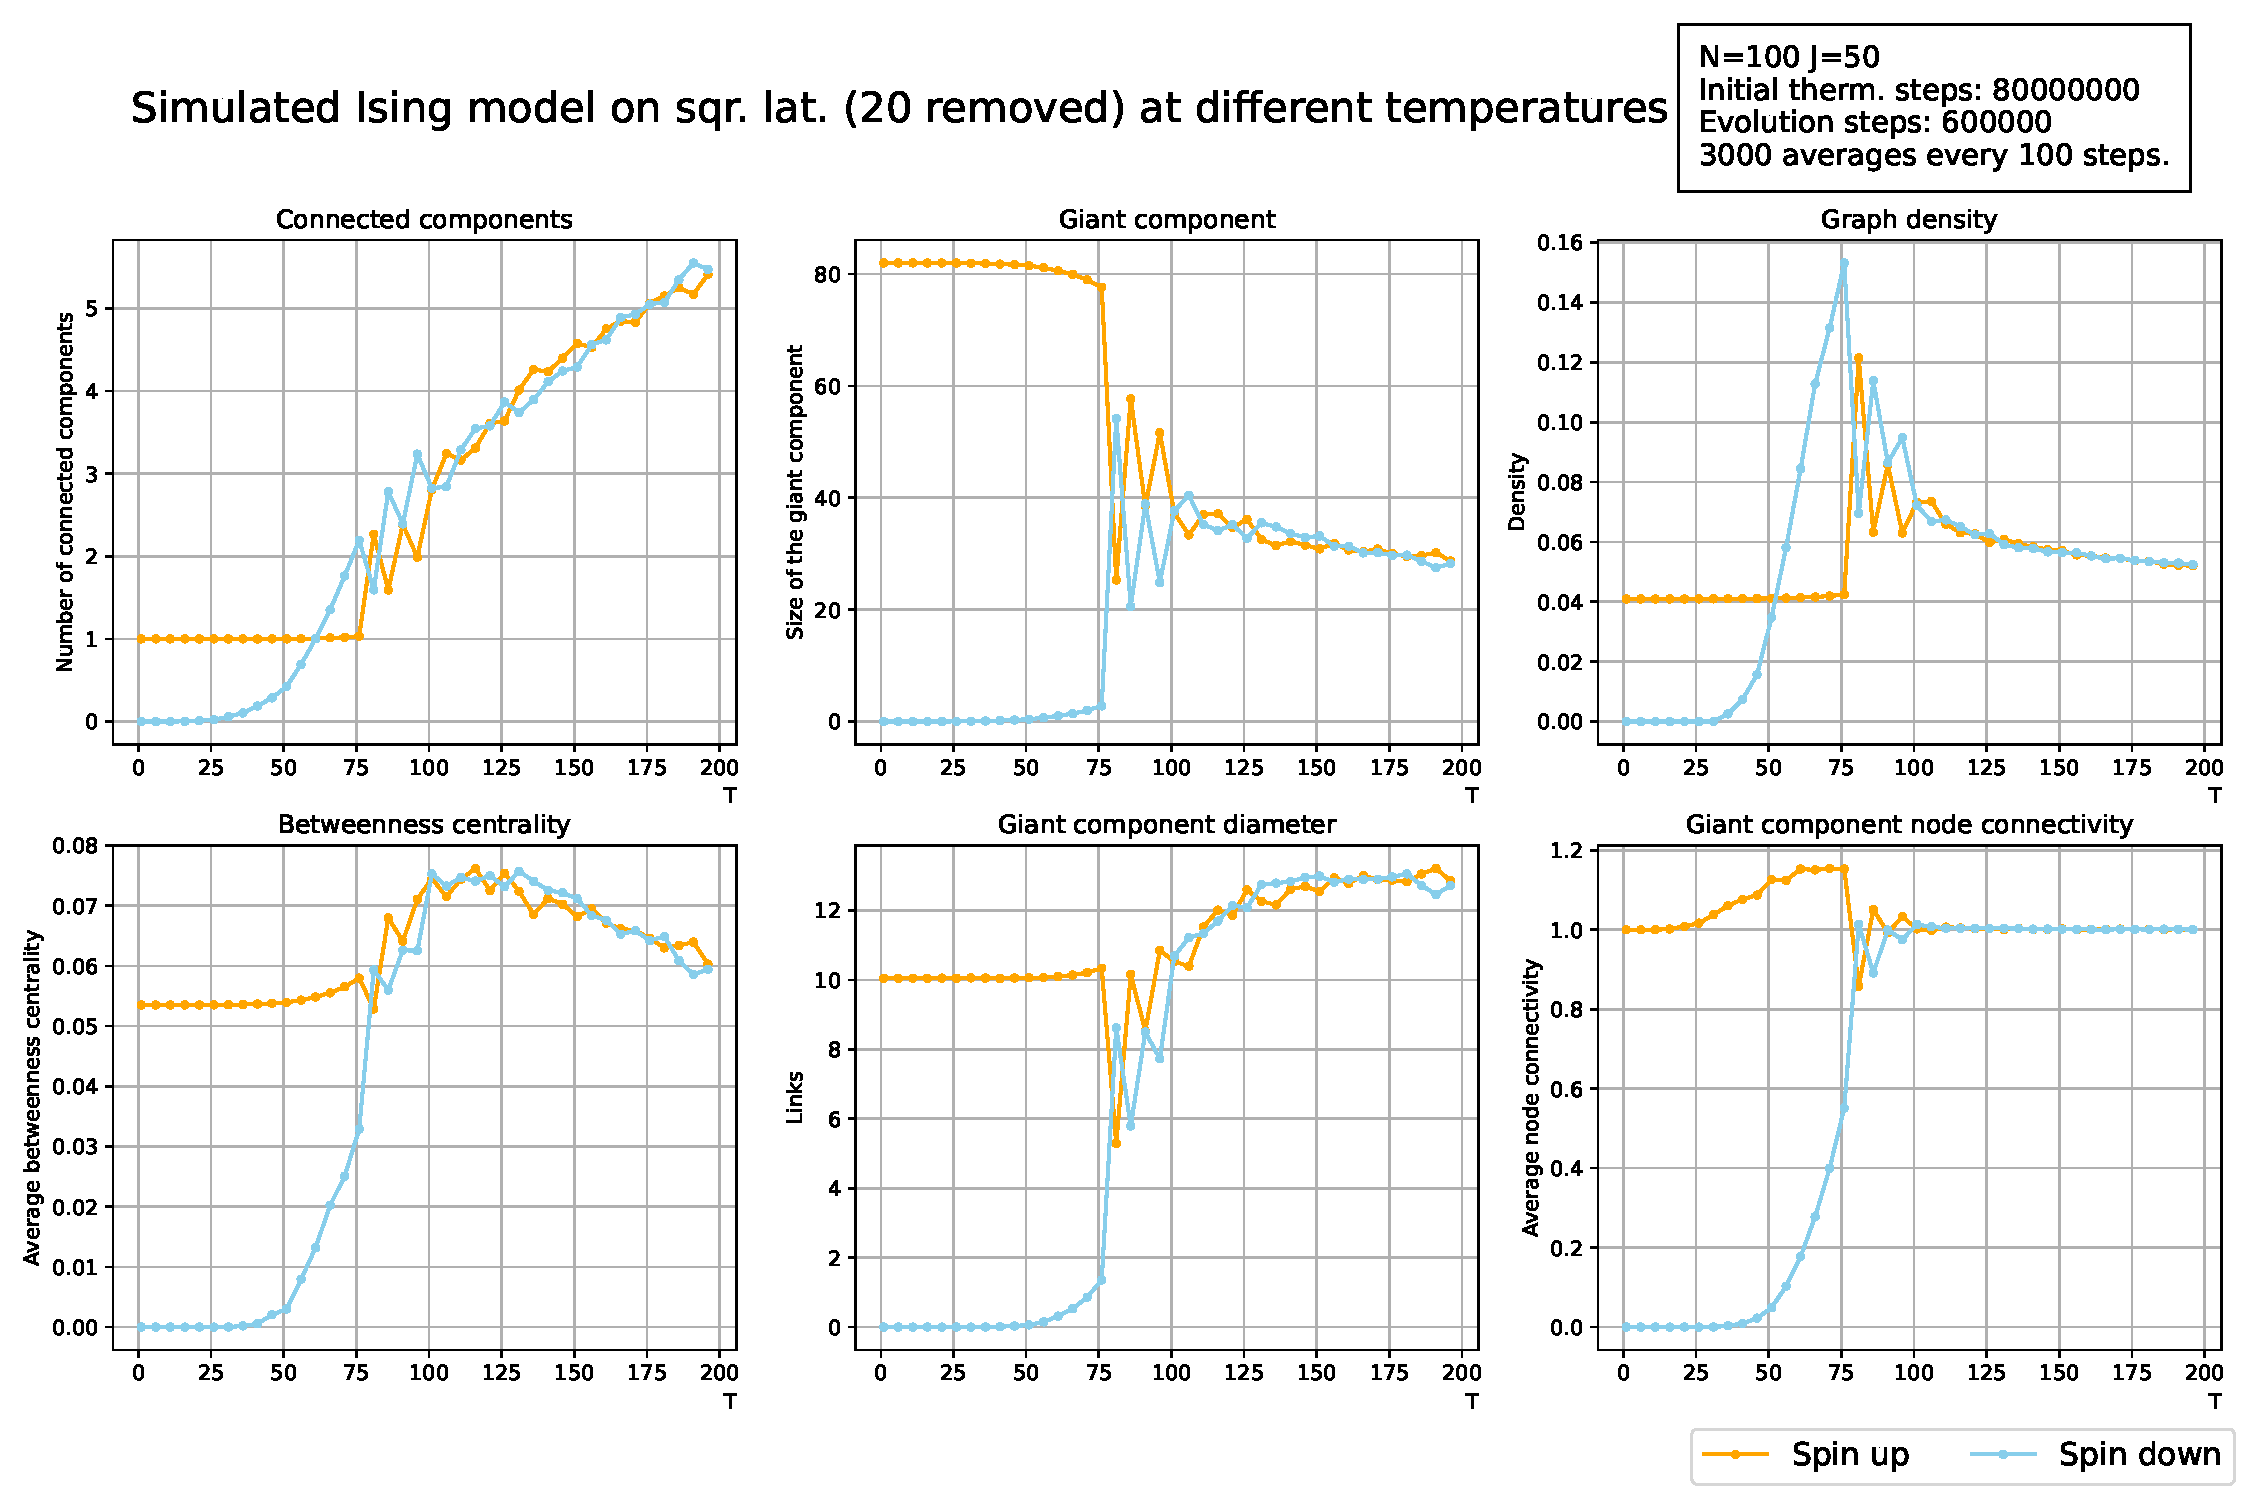
\includegraphics[width=.5\linewidth]{Broken/Square_20.pdf}
  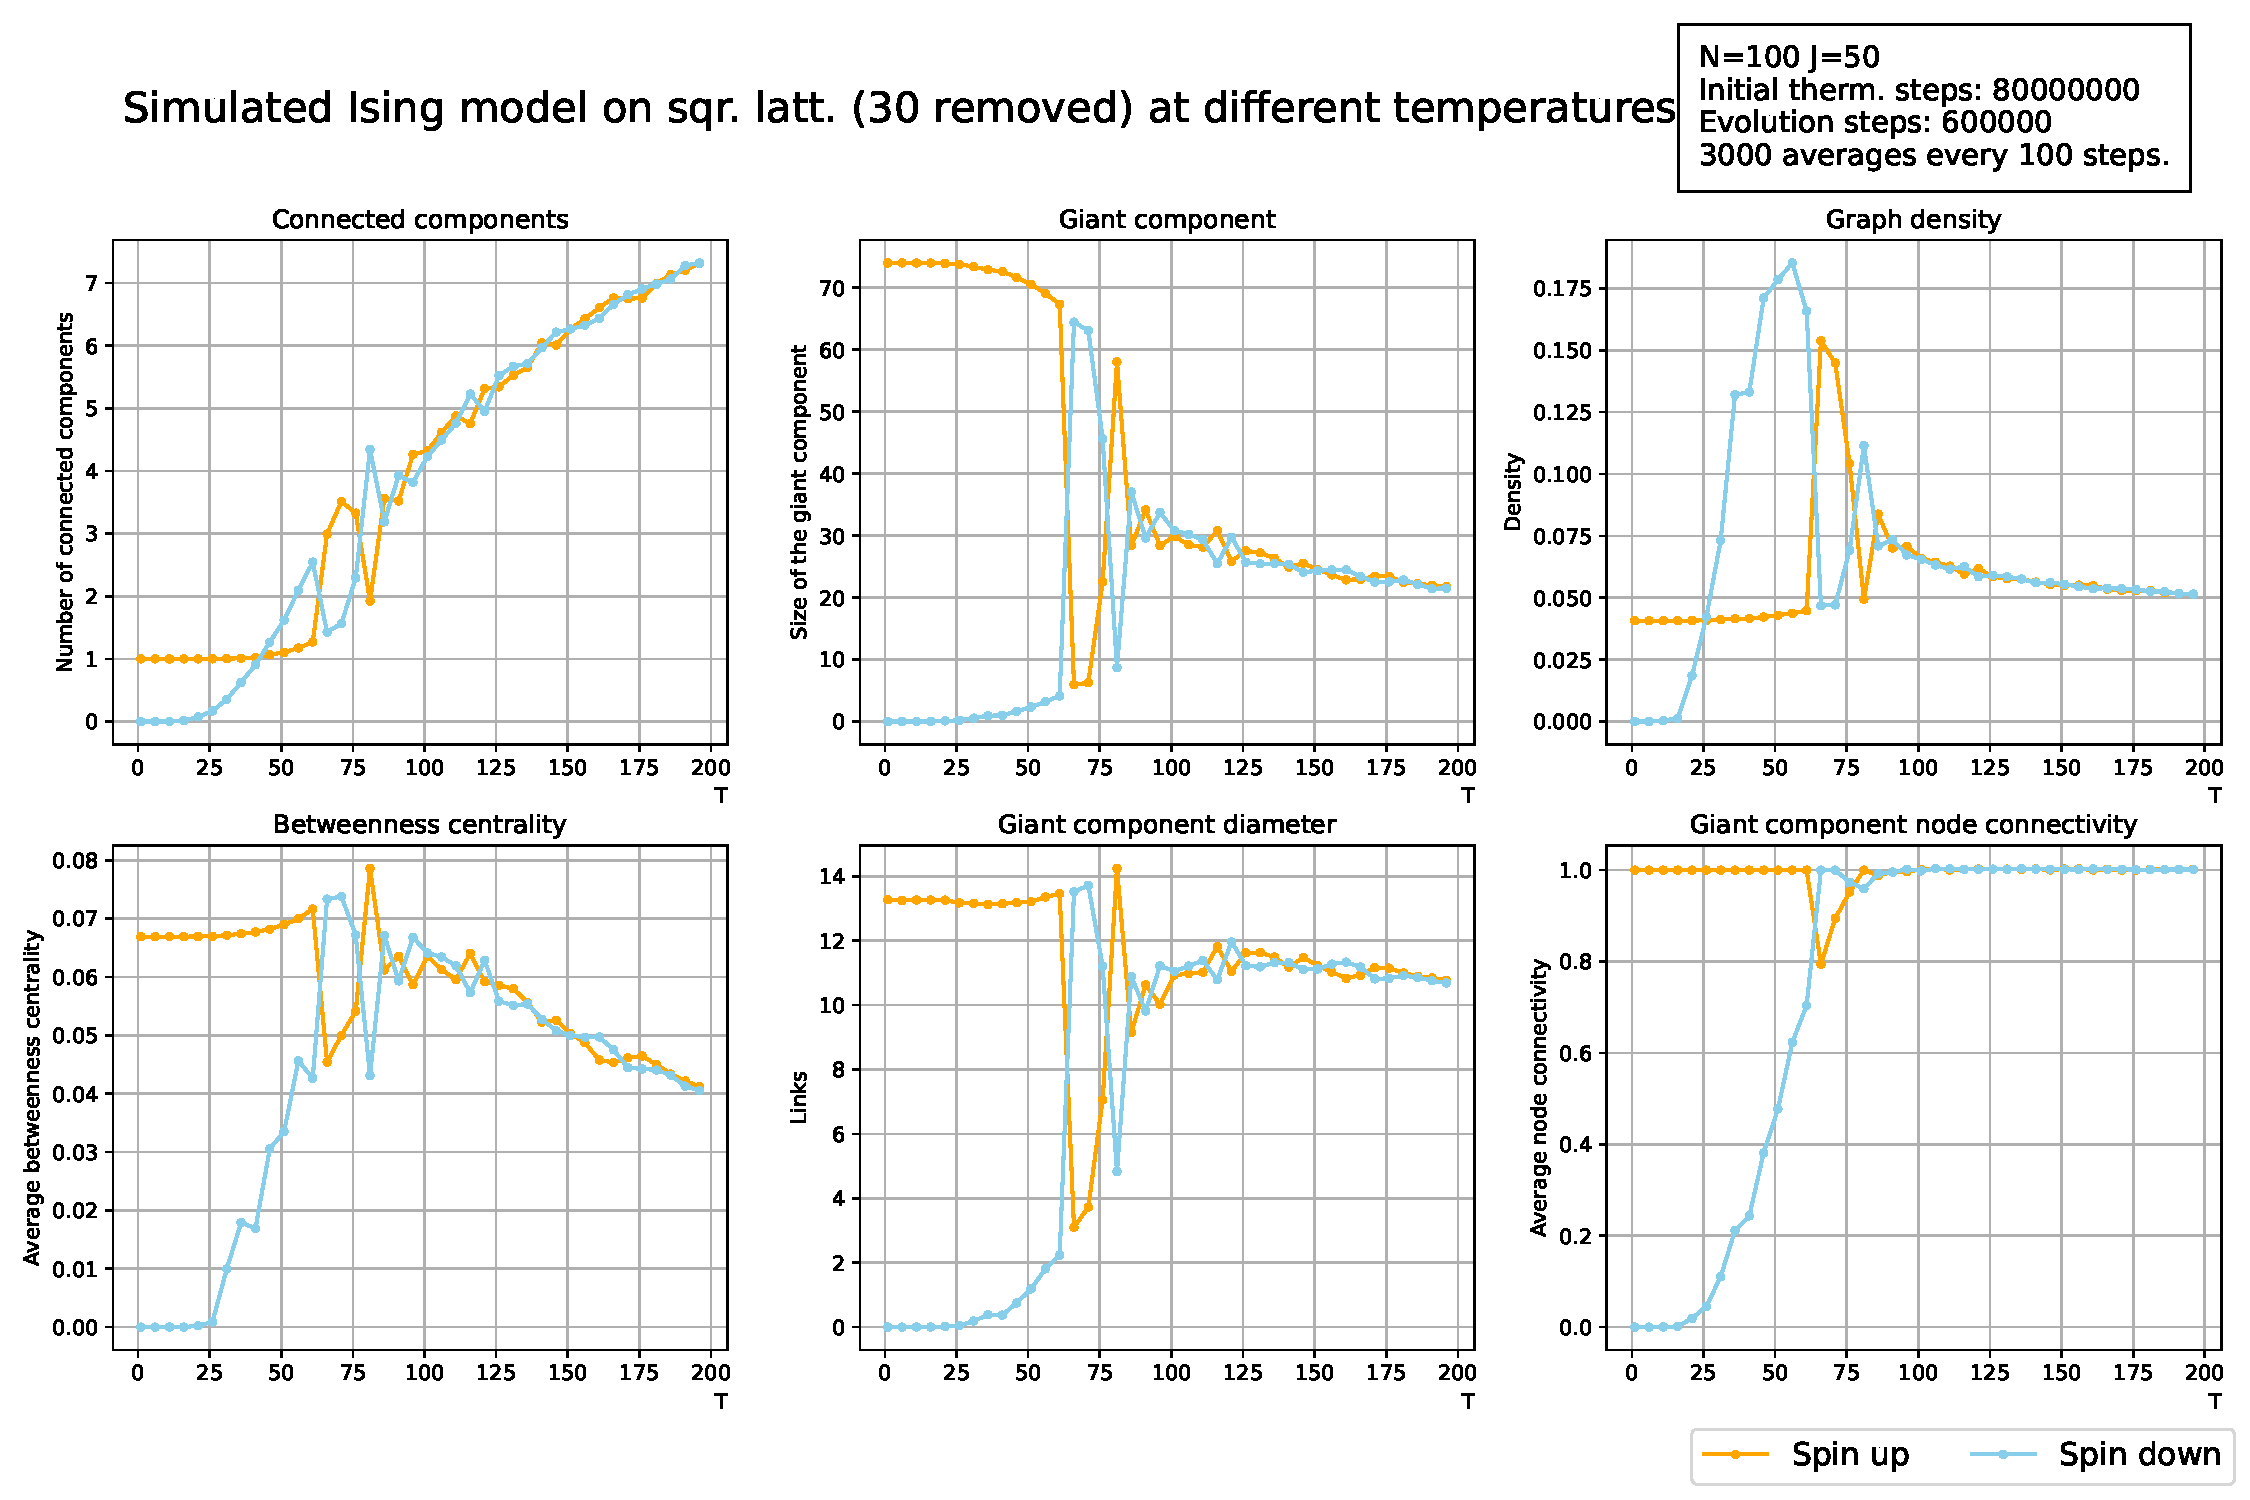
\includegraphics[width=.5\linewidth]{Broken/Square_30.pdf}
    \caption{Behavior of the network proprieties of a square lattice from which we removed 7 atoms. The orange line is the spin up network while the blue is the spin down one.}
    \label{Fig:BSNetworkmeasure}
\end{figure}

\subsubsection*{Herdos-Renyi}
The Herdos-Renyi lattice simulation appears to be different from the other ones: after the phase transition the number of connected components per type of spin increases a little without never showing a clear split in 2 or more components, and also the size of the giant components shows that the lattice is almost perfectly split in two domains. We can also note that the giant component connectivity never drops to 1, as it used in the other lattices. We must conclude that a Herdos-Renyi network is too much connected to generate more tree-like connected components, even though the betweenness centrality still rises after the phase transition. This increment of the betweenness centrality is coherent with the node connectivity, which halves, signaling that the networks becomes less connected but not as much as the previous networks.  
\begin{figure}[!htb]
  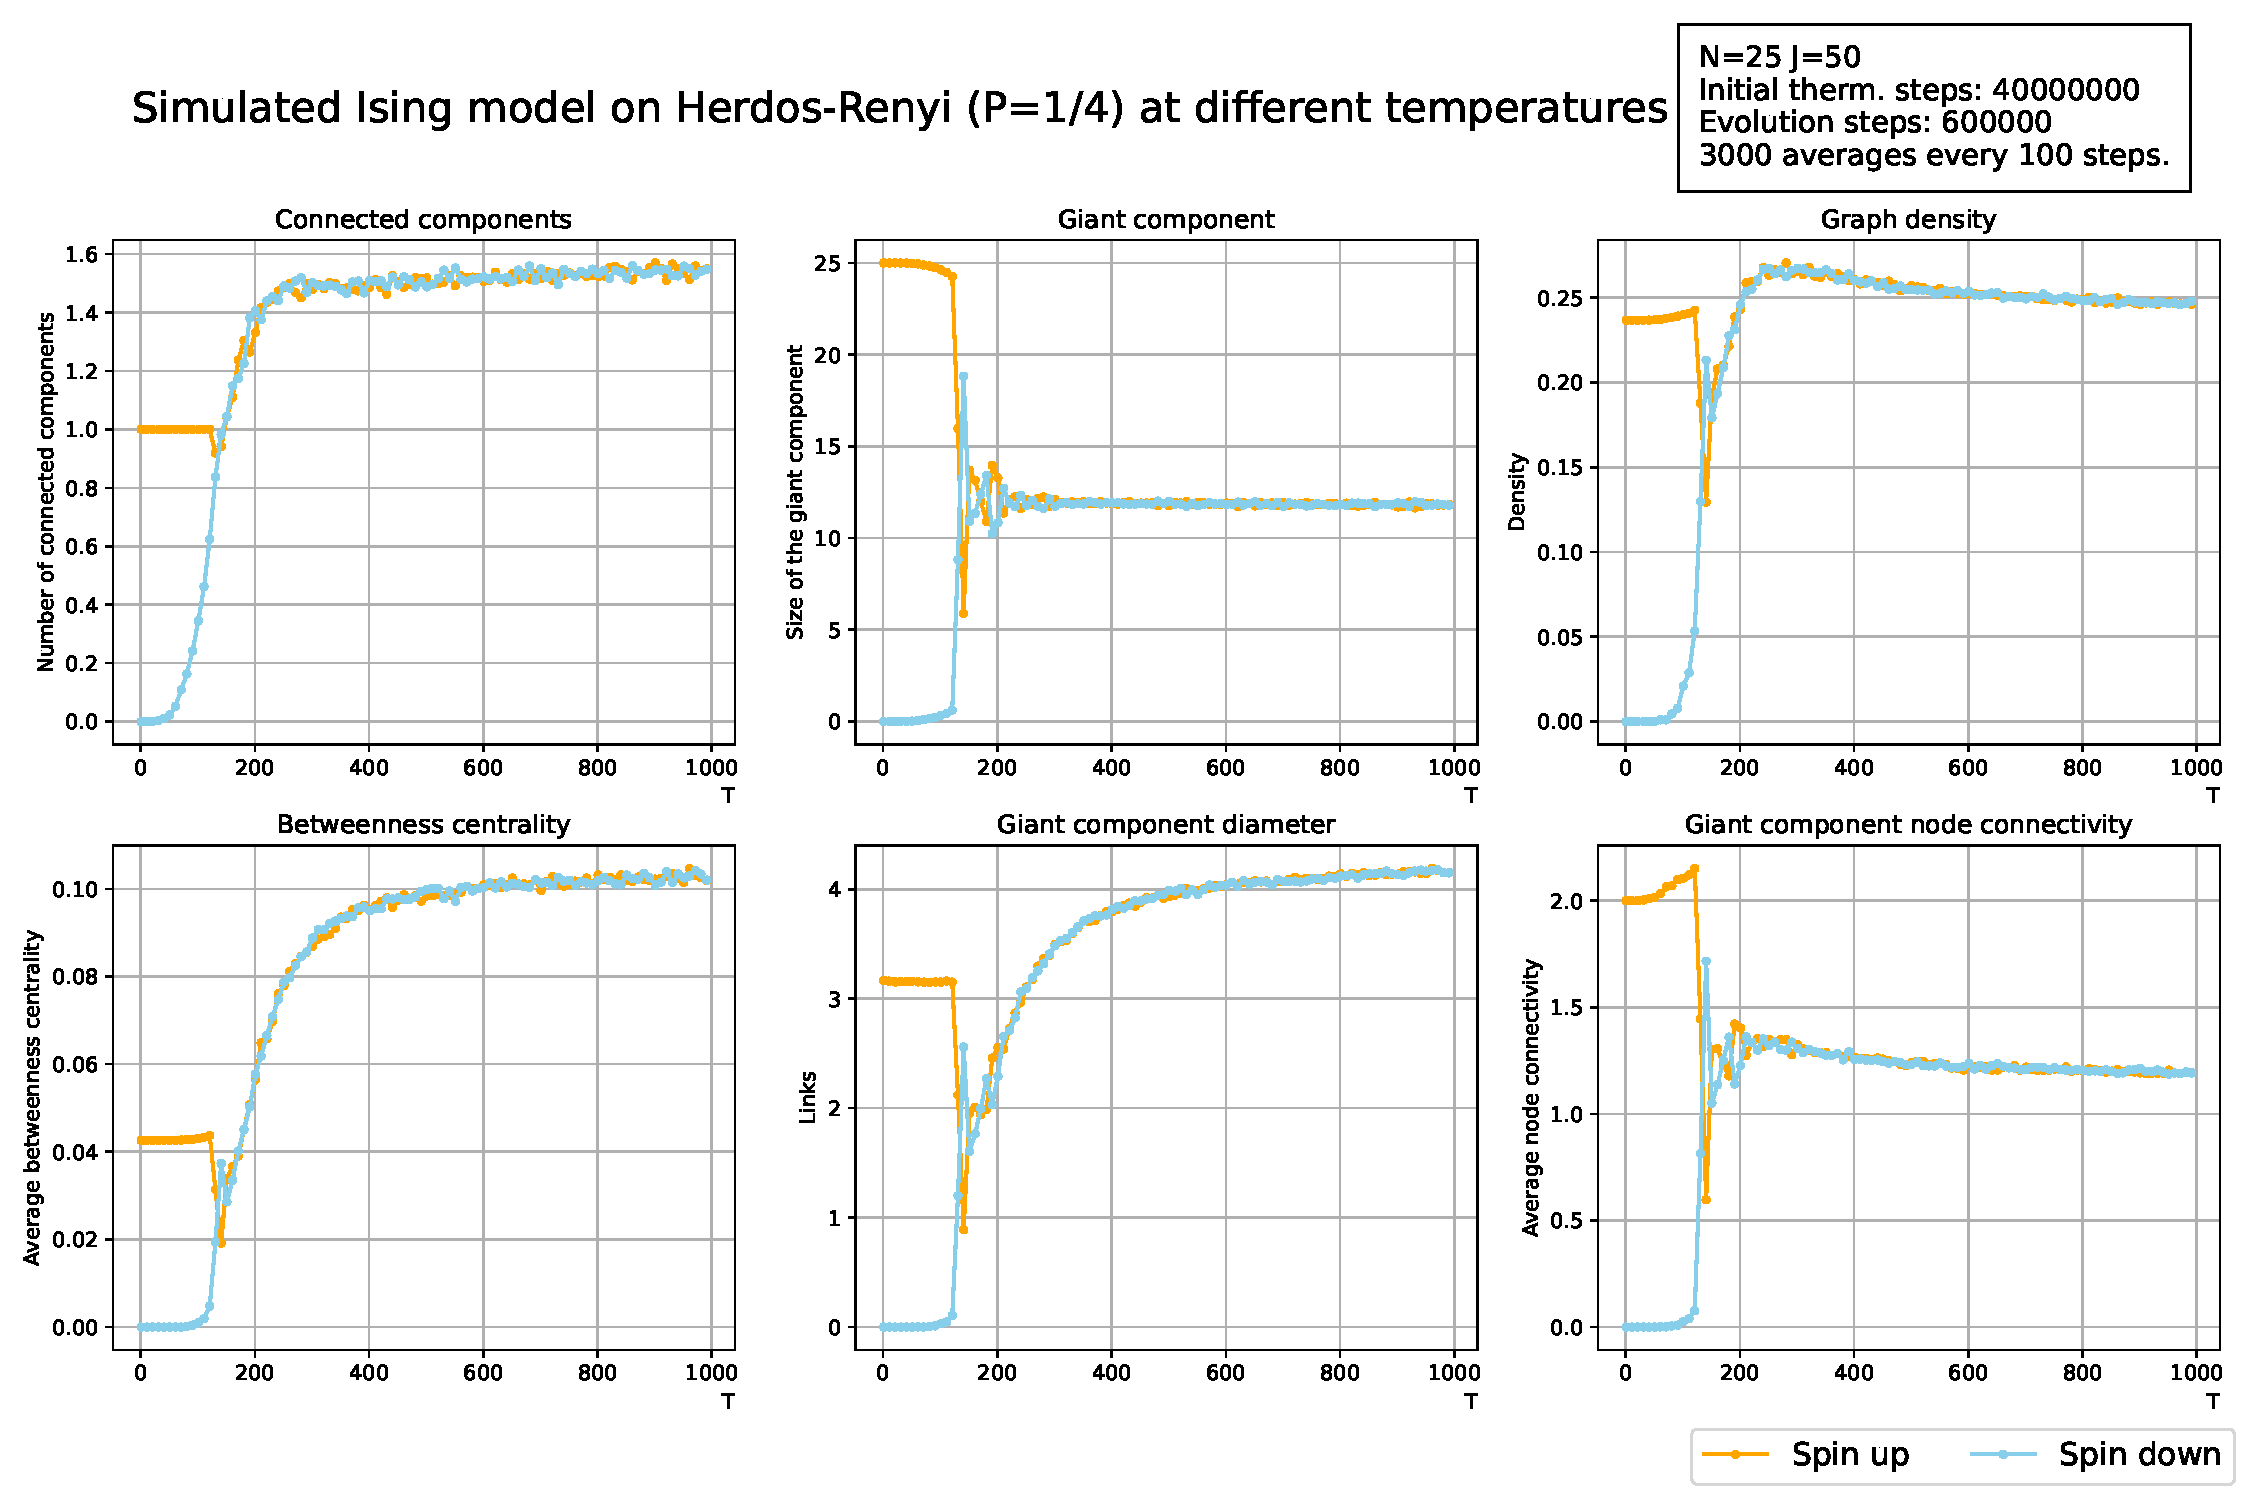
\includegraphics[width=\linewidth]{Network meausres/HR.25_Network.pdf}
    \caption{Behavior of the network proprieties of the Herdos-Renyi lattice at increasing temperatures. The orange line is the spin up network while the blue is the spin down one.}
    \label{Fig:1RHNetworkmeasure}
\end{figure}
Figures \ref{Fig:1RHNetworkmeasure}, \ref{Fig:2RHNetworkmeasure}, \ref{Fig:3RHNetworkmeasure} show different Herdos-Renyi networks with increasing probability of having a link. At lower probability, which produce a graph with fewer edges, the phase transition is still similar to the ones on lattices (Fig. \ref{Fig:1RHNetworkmeasure}), however as we increase the links, by increasing their probability, the features that we already explained become more evident. 

We also noticed that, as we increased the links, the temperatures at which the symmetries of the system are restored starts to shift from the critical temperature that we measure thermodynamically. We can appreciate this shift observing that while transitioning sometimes spin-up and spin-down networks swap: one starts to behave as the other used in a coherent way but losing the information on which one was the original alignment at $T=0$. Meanwhile, the critical temperatures increase as the probability of generating a link increases.
\begin{figure}[!htb]
  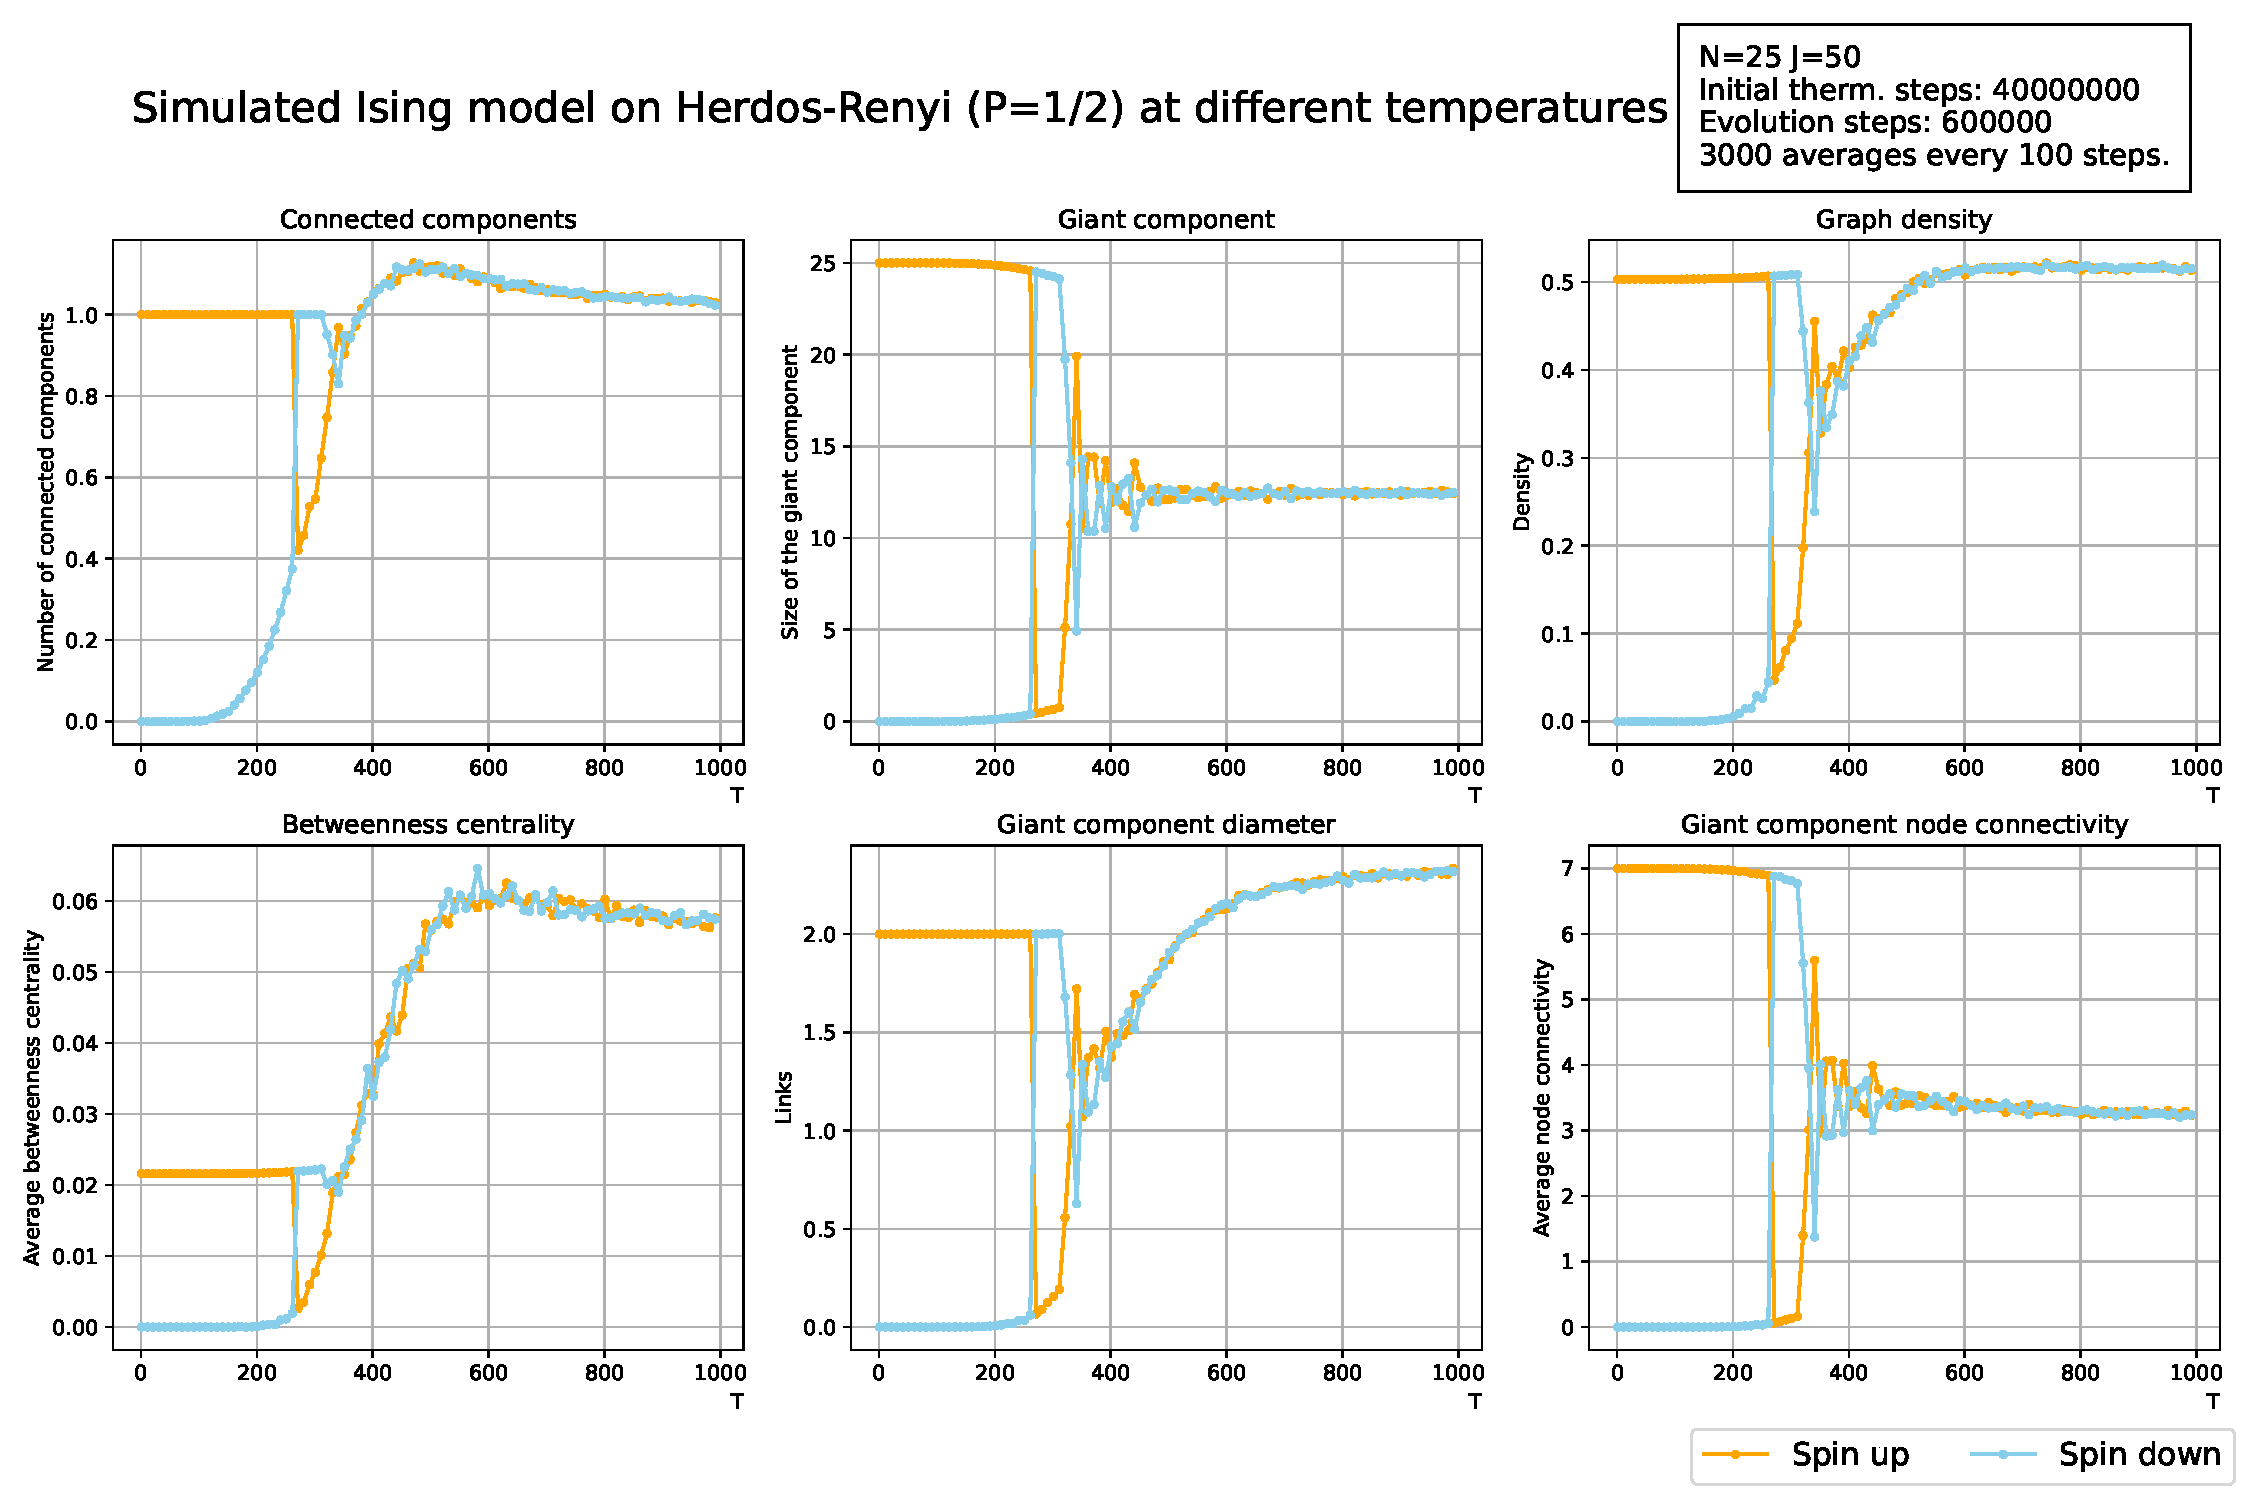
\includegraphics[width=\linewidth]{Network meausres/HR.5_Network.pdf}
    \caption{Behavior of the network proprieties of the Herdos-Renyi lattice at increasing temperatures. The orange line is the spin up network while the blue is the spin down one.}
    \label{Fig:2RHNetworkmeasure}
\end{figure}
\begin{figure}[H]
  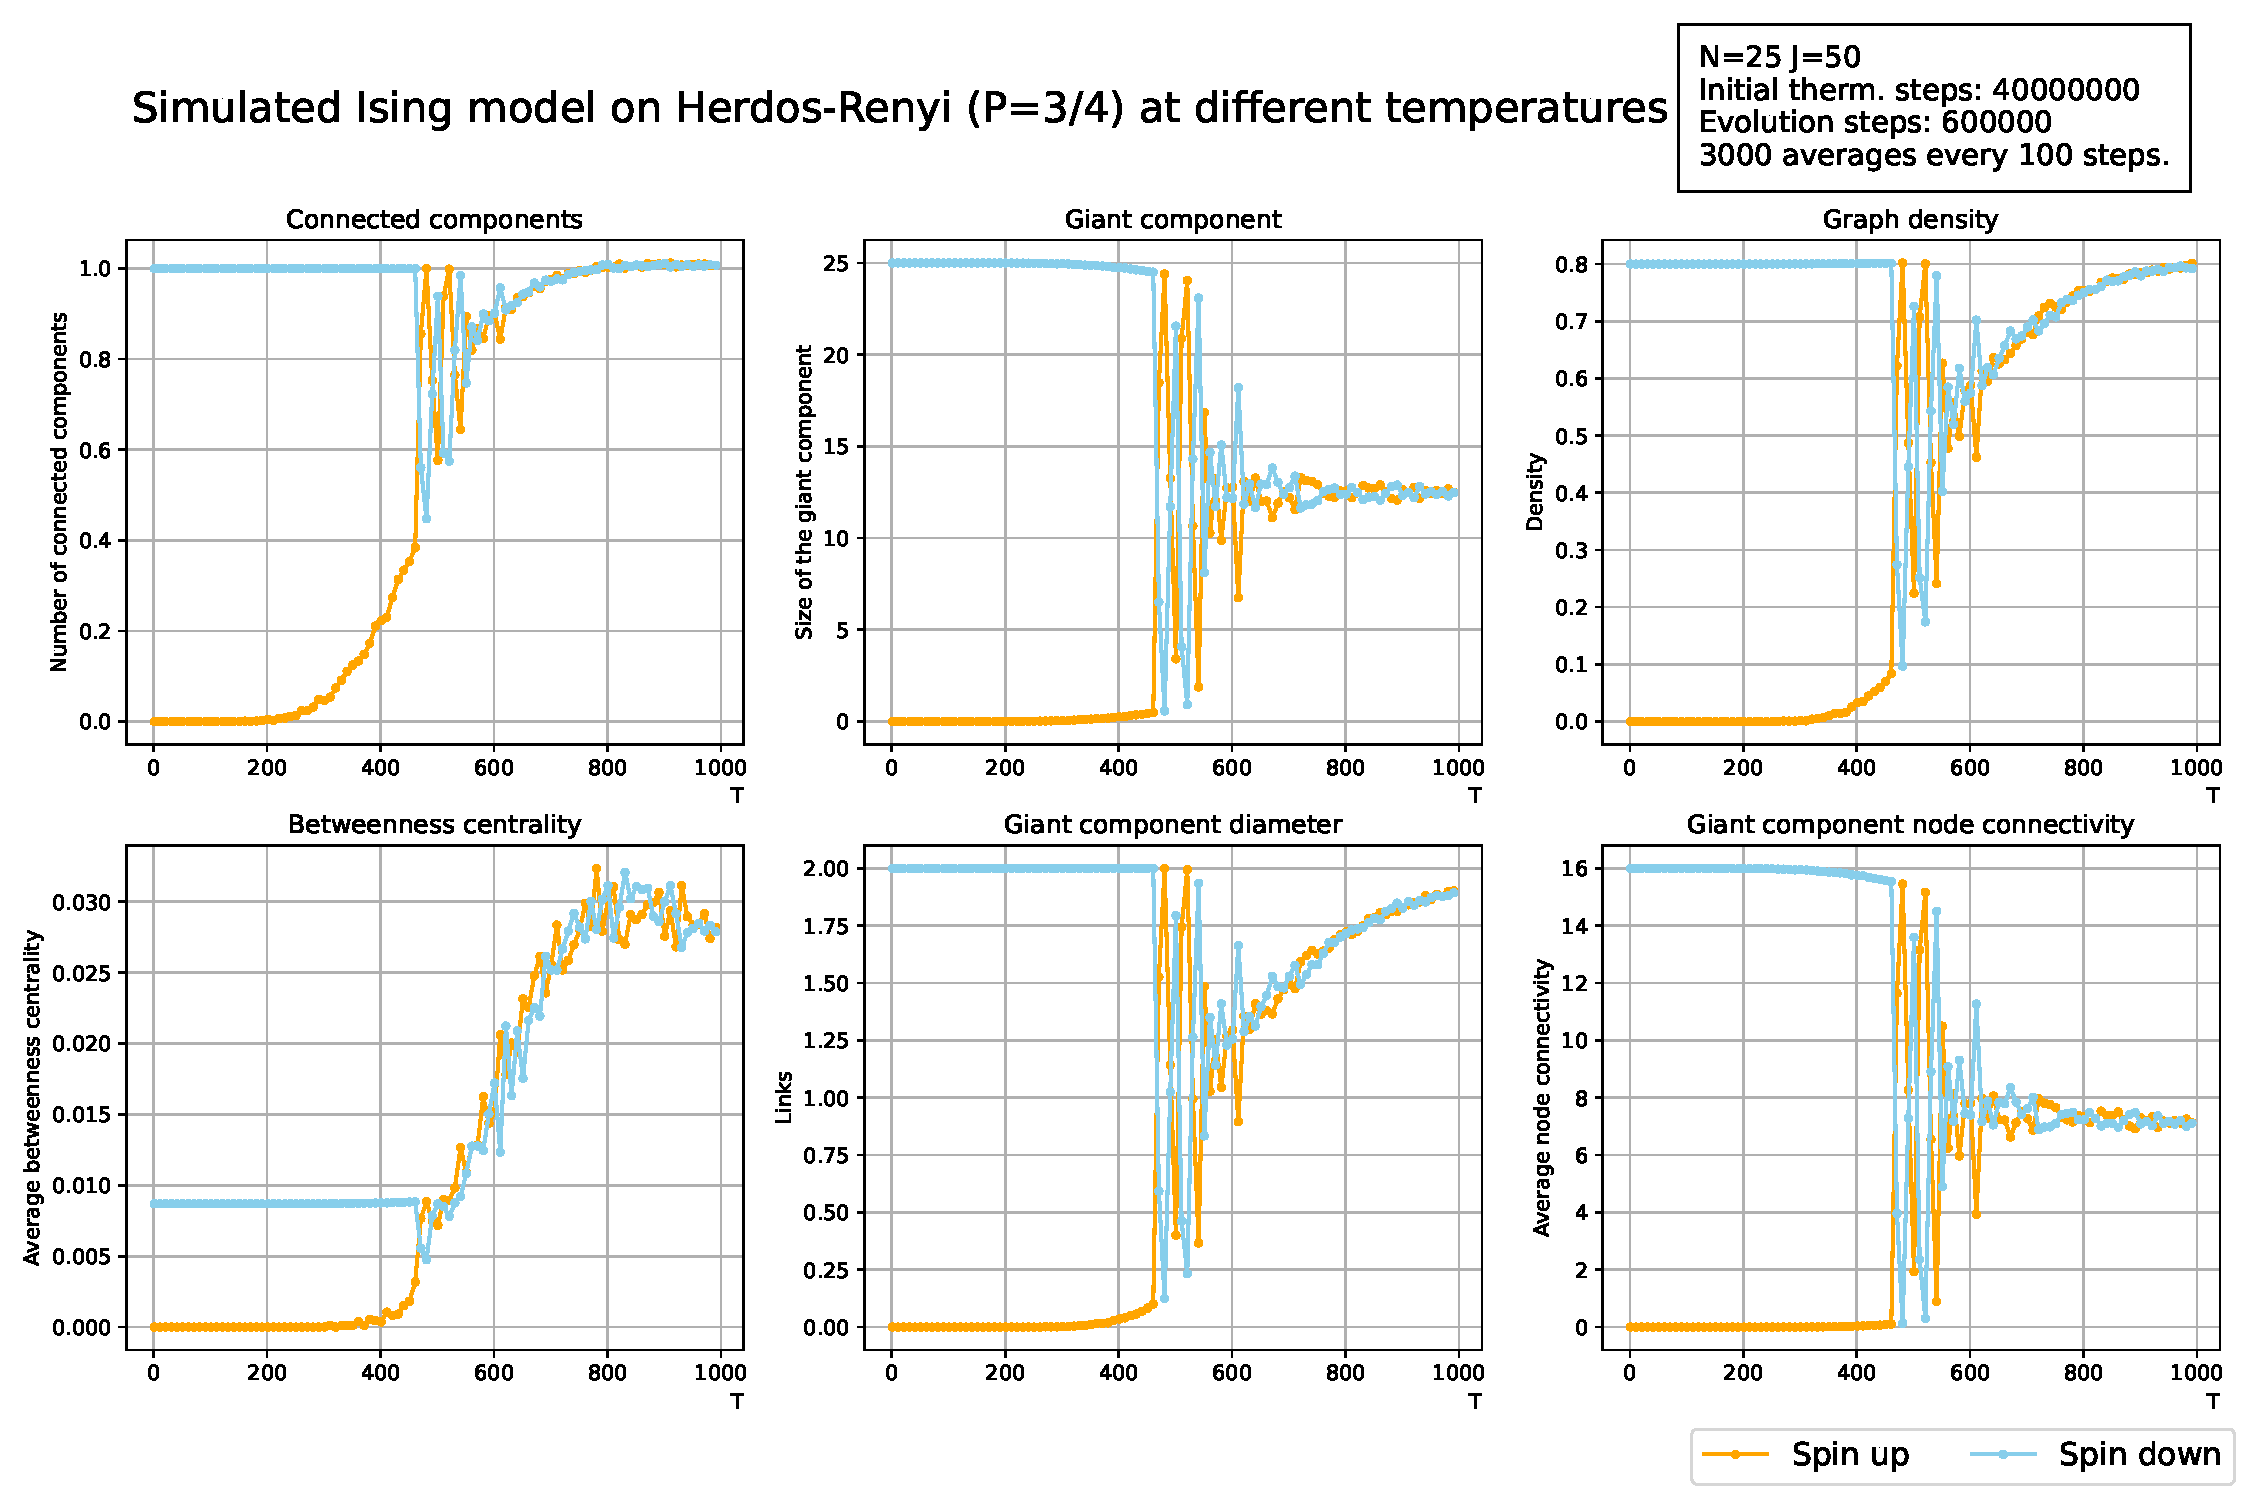
\includegraphics[width=\linewidth]{Network meausres/HR.75_Network.pdf}
    \caption{Behavior of the network proprieties of the Herdos-Renyi lattice at increasing temperatures. The orange line is the spin up network while the blue is the spin down one.}
    \label{Fig:3RHNetworkmeasure}
\end{figure}

\newpage 

\subsubsection*{More than nearest neighbor}
We also simulated the Ising model on lattices where are allowed interactions with the neighbors of the neighbors of each atom. This mimicked short range interactions but over higher distances. We simulated on square, triangular and hexagonal lattices, using parameters comparable  with the one we already used.

Figures \ref{Fig:MNN1}, \ref{Fig:MNN2}, \ref{Fig:MNN3} shows that this longer range interaction showed again a phase transition behavior: in all the lattices we encounter two networks (spins up and spins down) behaving in completely different ways at lower temperatures but becoming completely indistinguishable at higher ones. However, we noticed that these transitions happen at higher temperatures than the normal ones (just nearest neighbors interactions). Furthermore, we noticed that these networks didn't break as much as the regular ones: at higher temperatures they simply divide into two connected components, one of spins up and the other of down.

\begin{figure}[!htb]
  \centering
  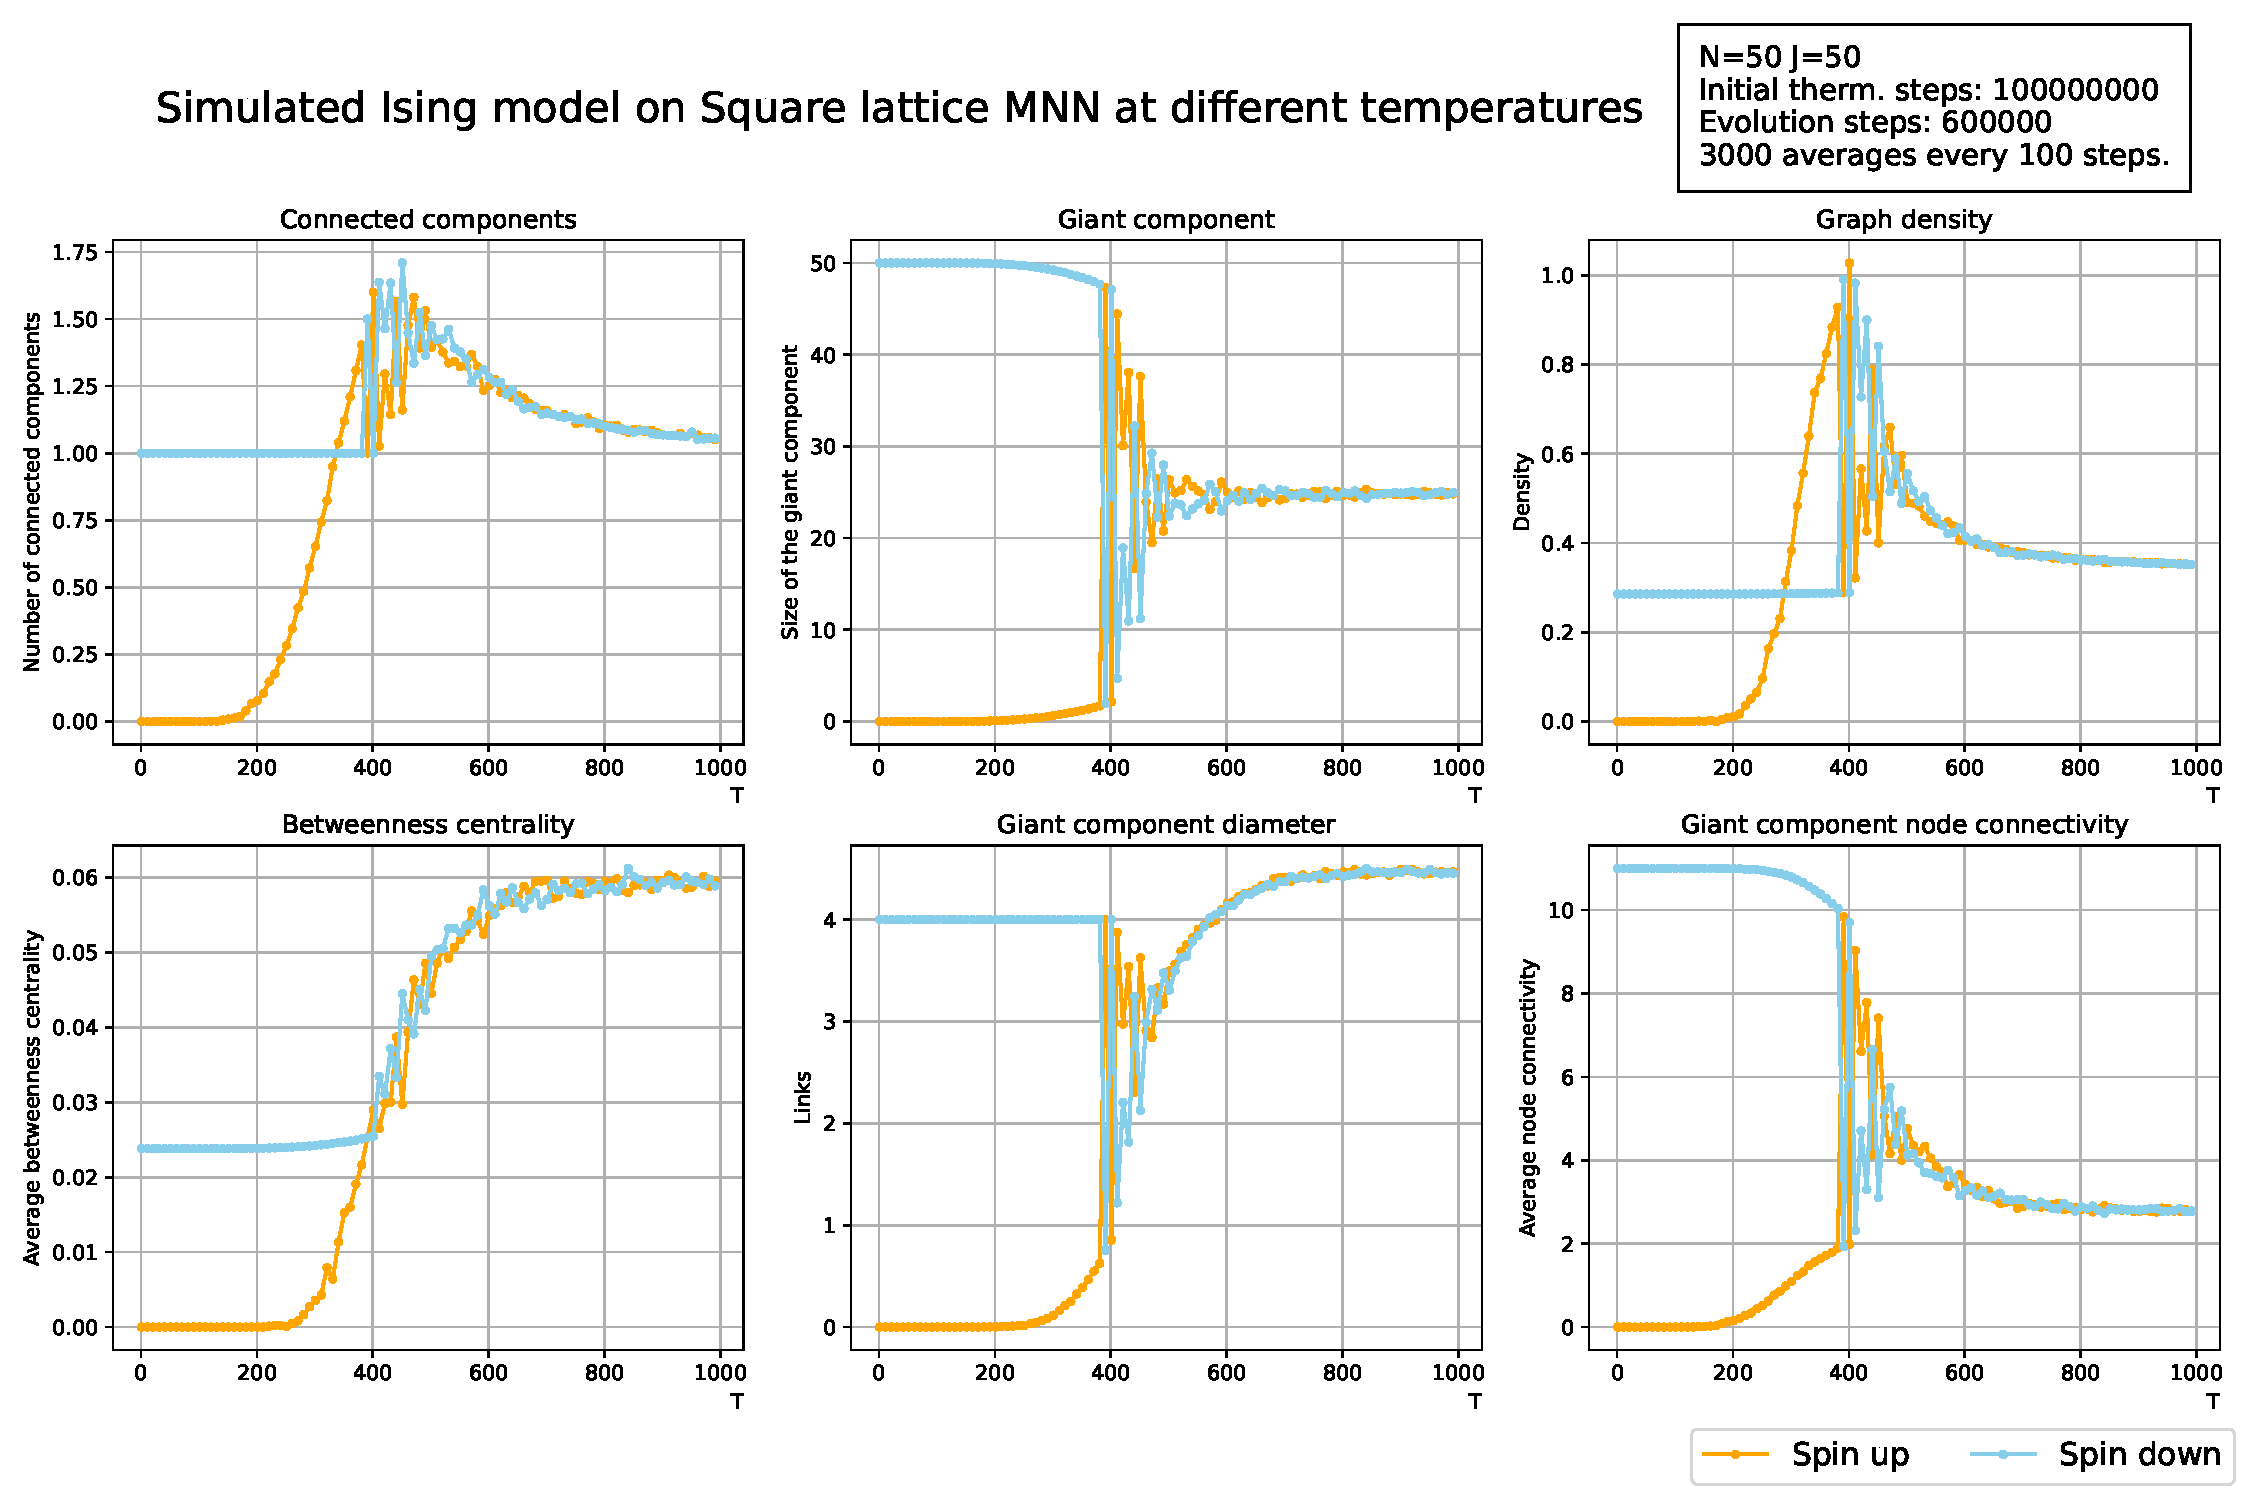
\includegraphics[width=\linewidth]{Network meausres/MNN_Square.pdf}
    \caption{Network proprieties of hexagonal lattice with more than nearest neighbor interactions. The orange line is the spin up network while the blue is the spin down one.}
    \label{Fig:MNN1}
\end{figure}
\begin{figure}[!h]
  \centering
  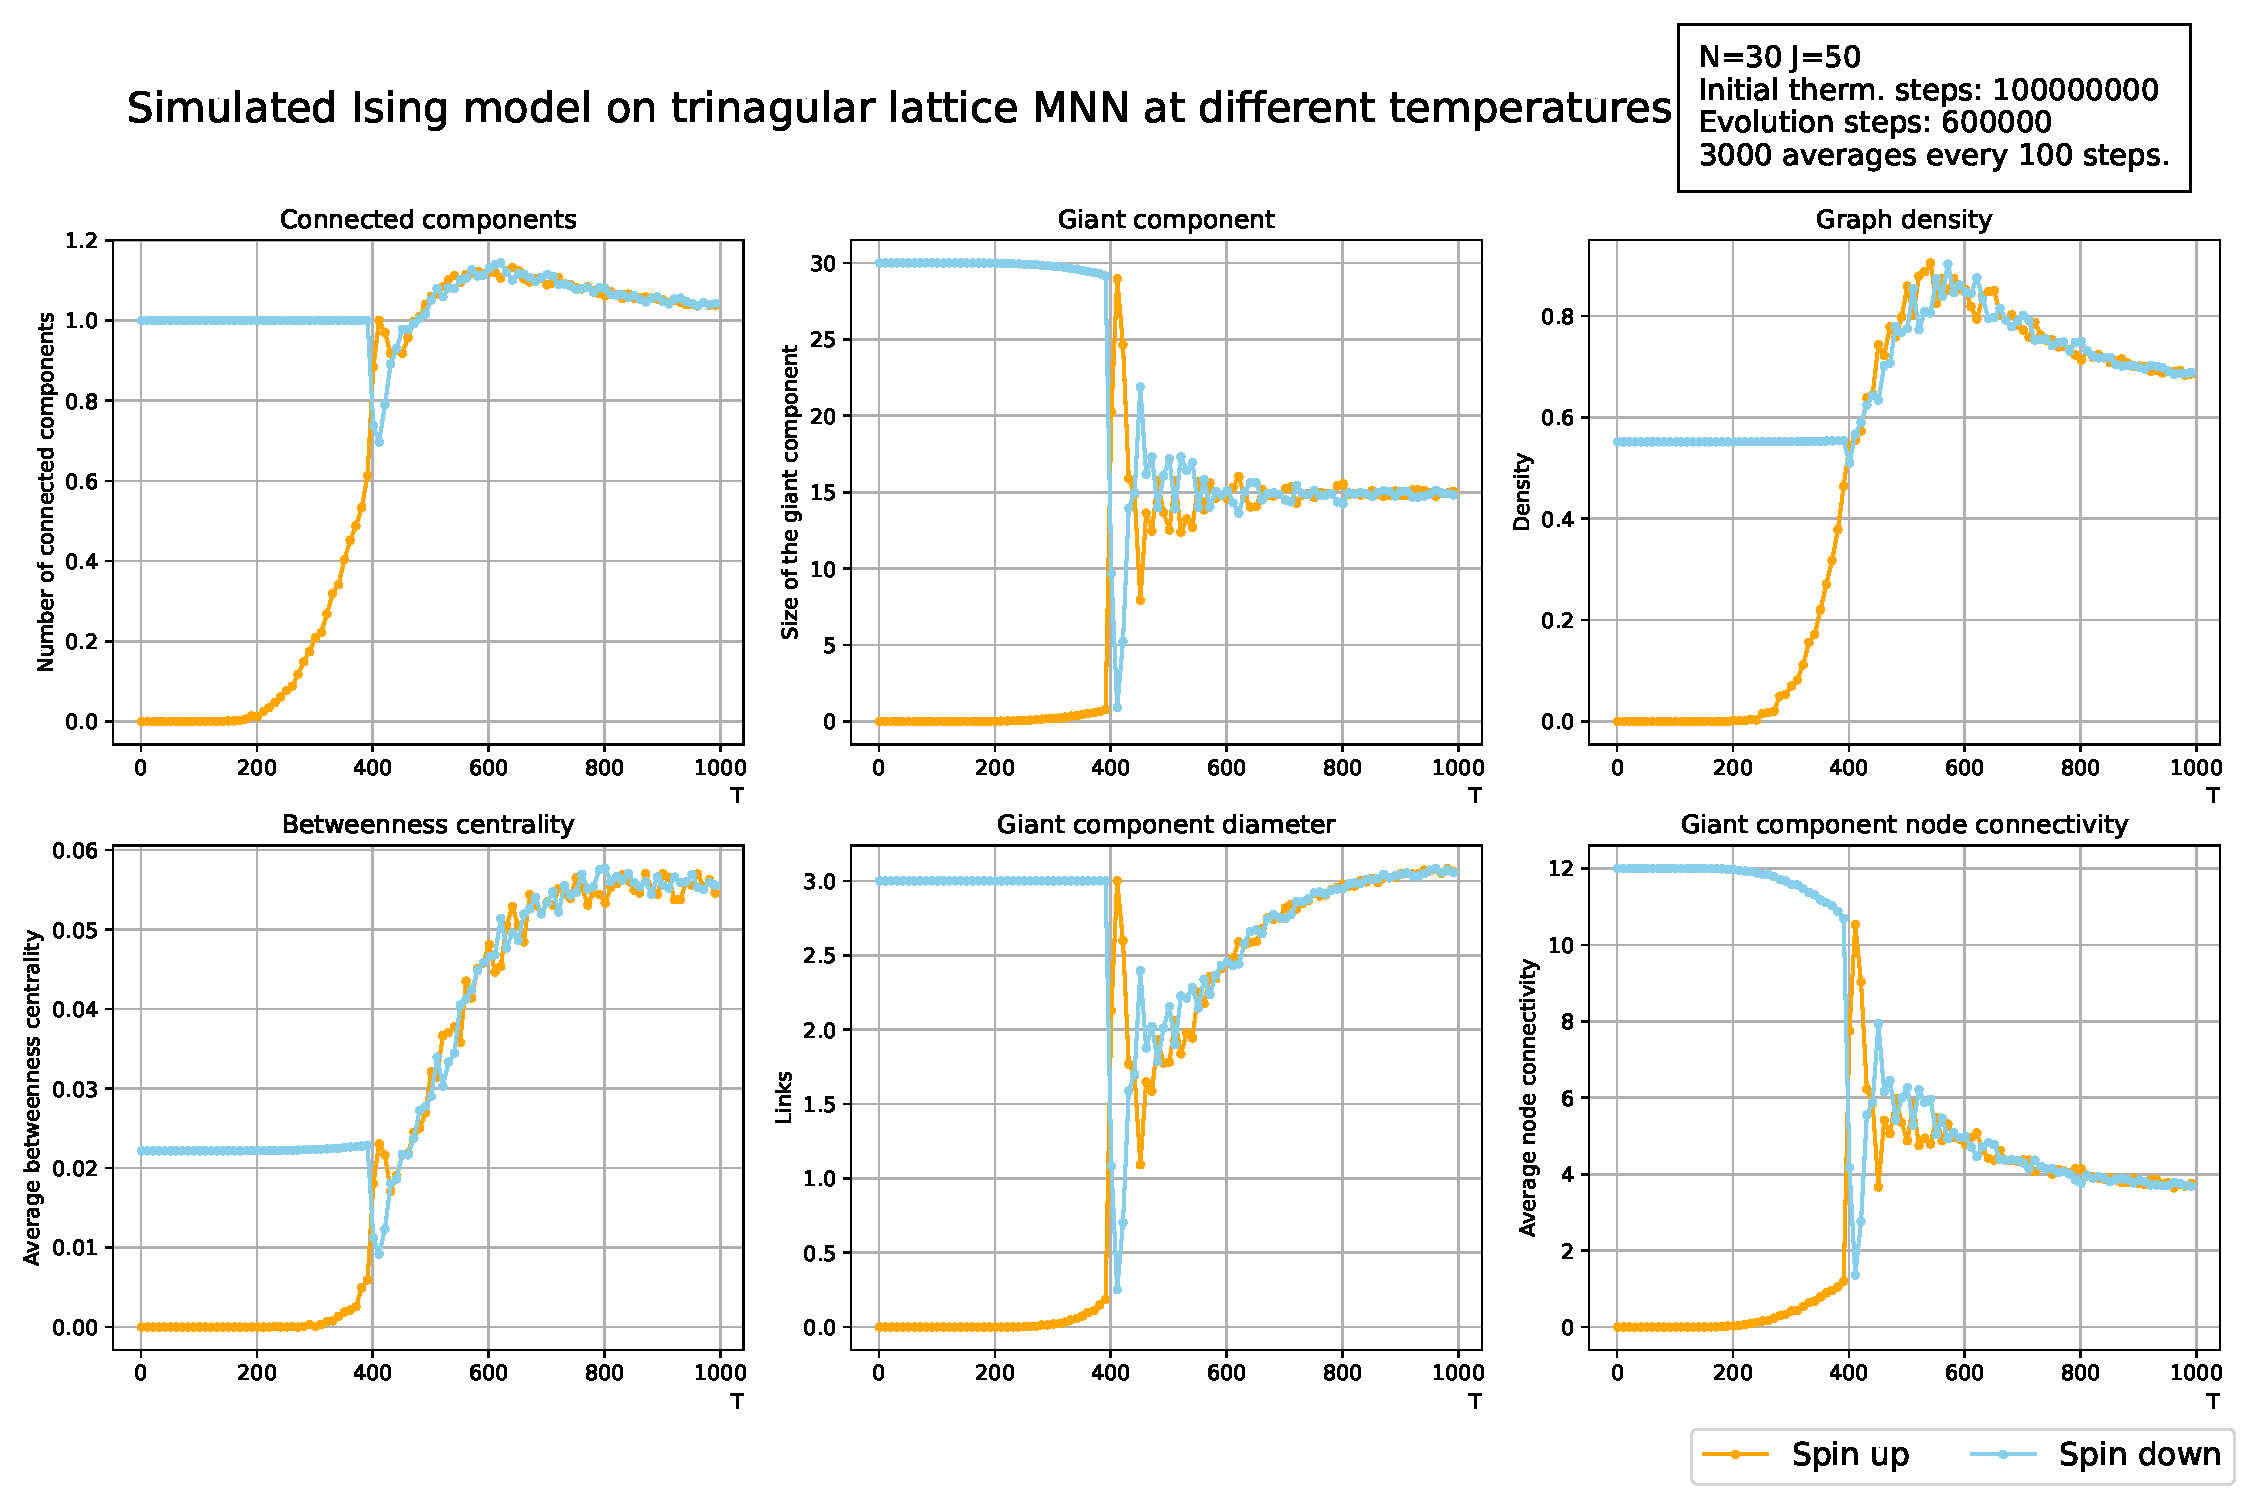
\includegraphics[width=\linewidth]{Network meausres/MNN_Triang.pdf}
    \caption{Network proprieties of hexagonal lattice with more than nearest neighbor interactions. The orange line is the spin up network while the blue is the spin down one.}
    \label{Fig:MNN2}
\end{figure}
\begin{figure}[H]
  \centering
  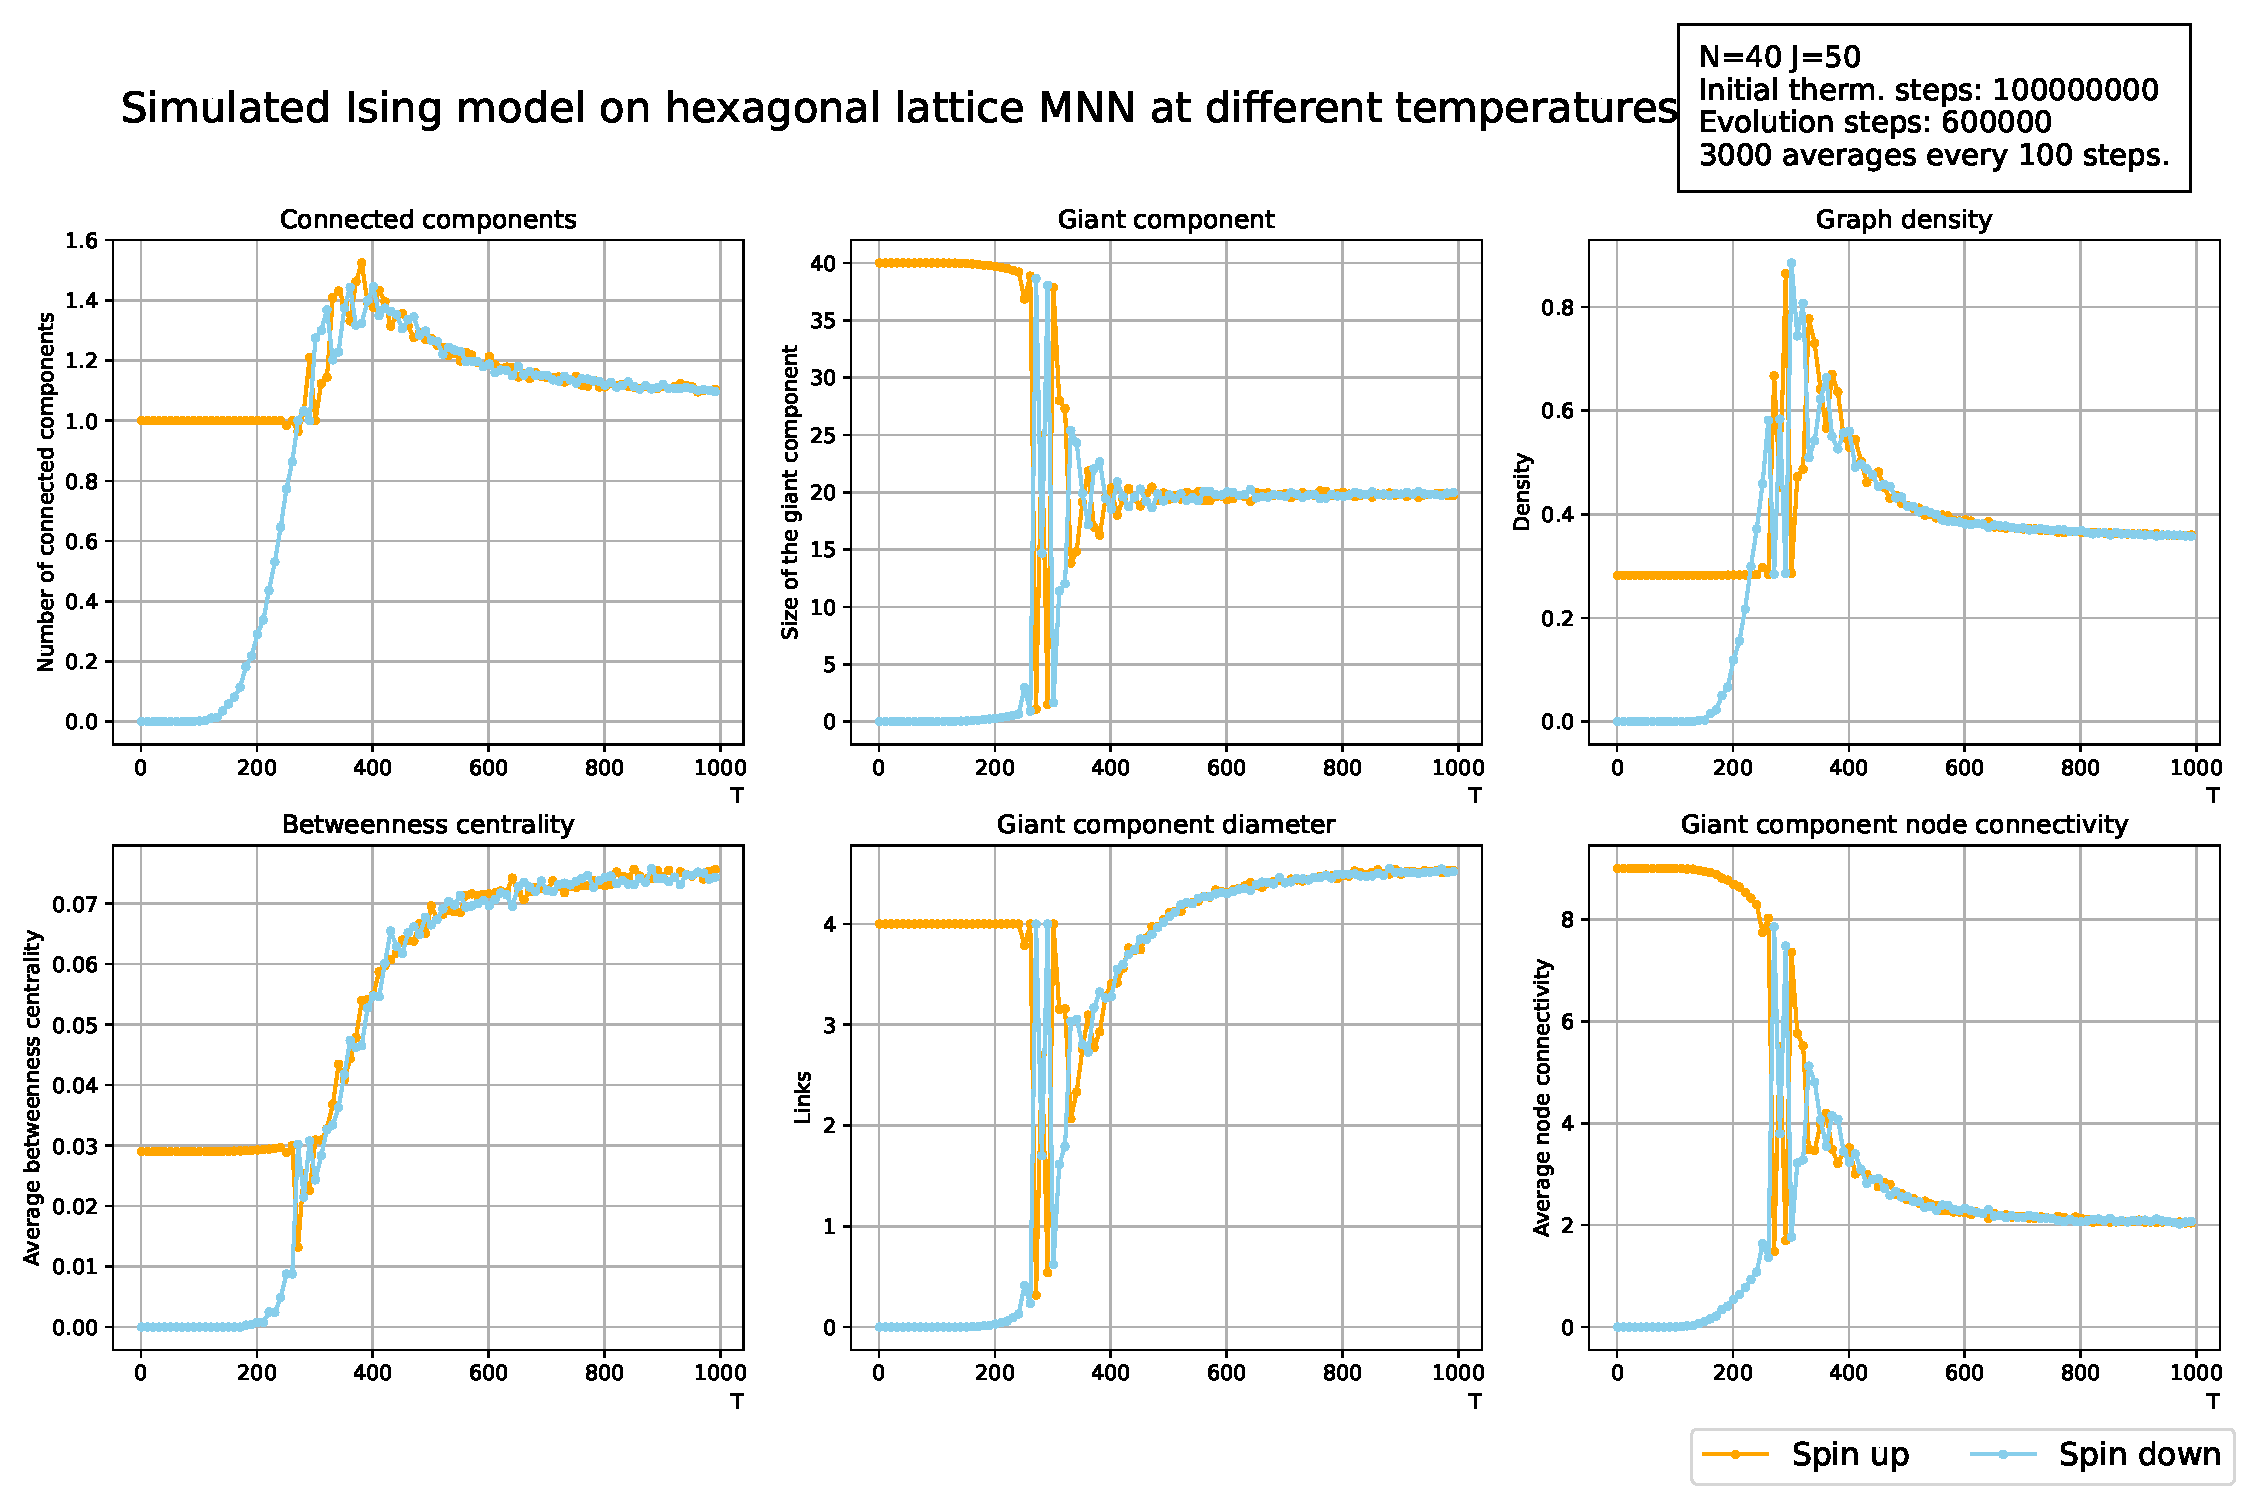
\includegraphics[width=\linewidth]{Network meausres/MNN_Hexa.pdf}
    \caption{Network proprieties of hexagonal lattice with more than nearest neighbor interactions. The orange line is the spin up network while the blue is the spin down one.}
    \label{Fig:MNN3}
\end{figure}
\newpage
\subsubsection*{1-D lattice}
The last simulation we tried is the 1-D lattice. This system is interesting because the exact solution of the Ising model predicts the absence of a phase transition. However, as Figure \ref{Fig:1-D} shows, in our simulation occurred a phase transition at low temperature in both circular graphs (closed loops) and open chains. This is probably due to the small number of atoms that we used.
\begin{figure}[H]
  \centering
  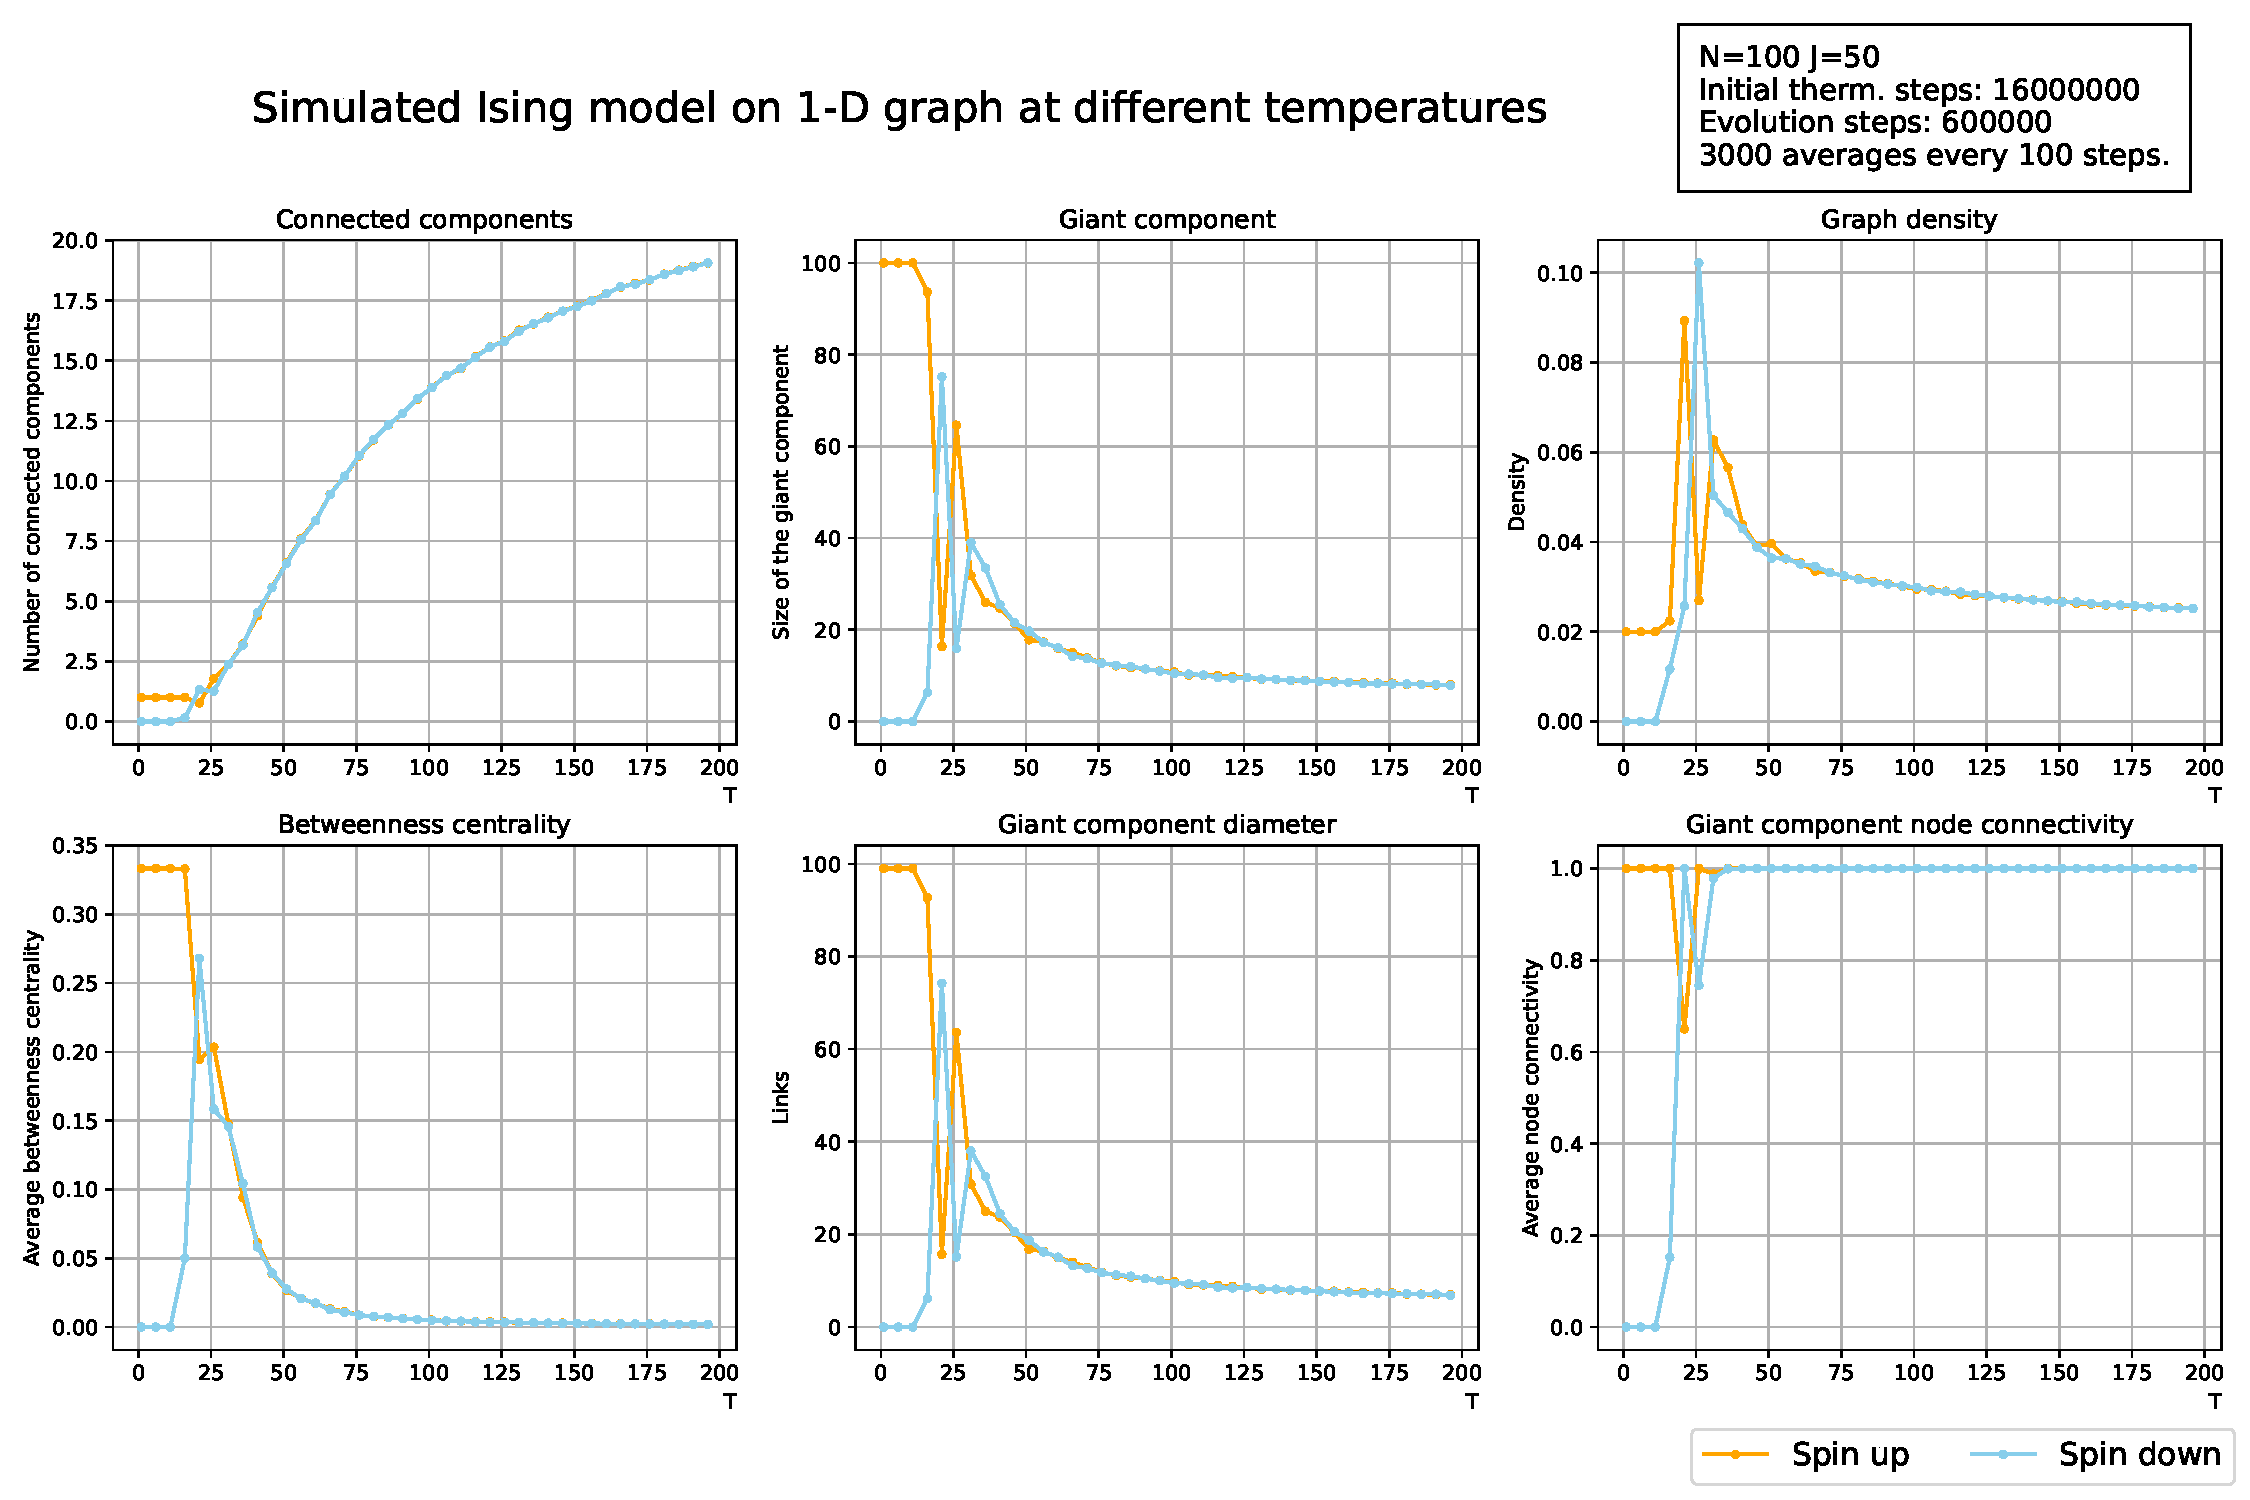
\includegraphics[width=.9\linewidth]{Network meausres/1-D100.pdf}
  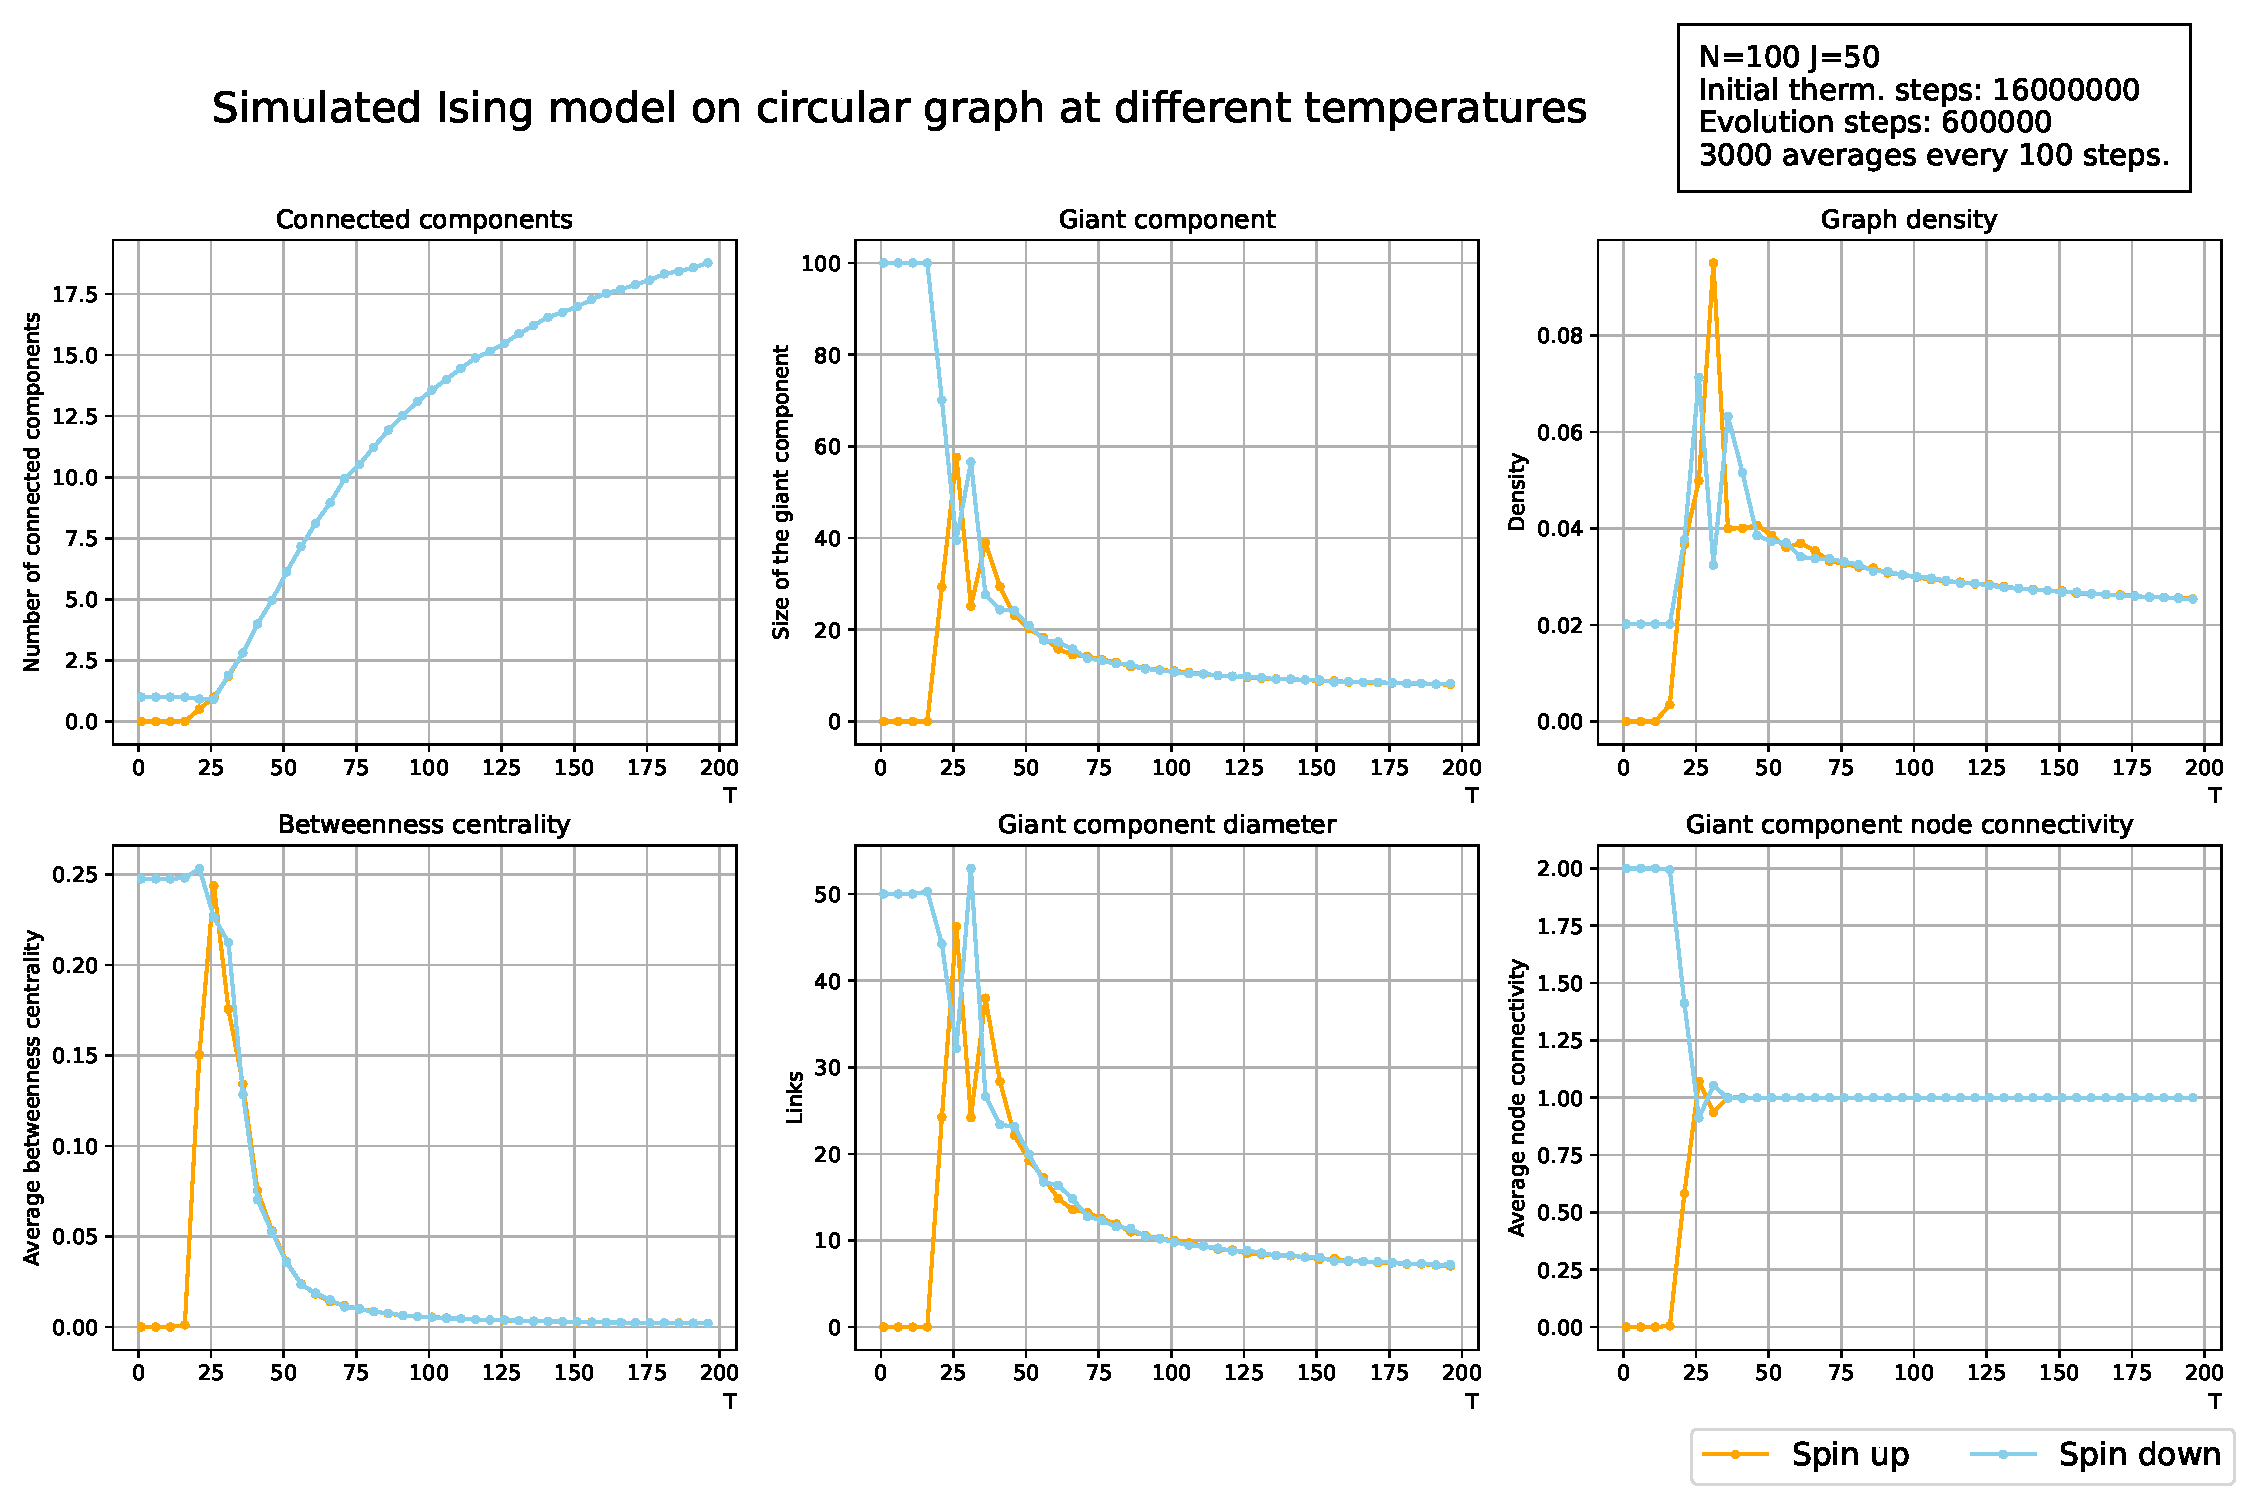
\includegraphics[width=.9\linewidth]{Network meausres/Circular100.pdf}
    \caption{Behavior of the network proprieties of a 1-D lattice and a circular graph at increasing temperatures. The orange line is the spin up network while the blue is the spin down one.}
    \label{Fig:1-D}
\end{figure}
